% Memorised Blades -- IEEE journal version.
% Build:  cd paper/ieee && latexmk -pdf main.tex      (pdflatex + bibtex; figures from ../figures, diagrams in tikz/)
% Every number is traceable to research_log.md and runs/analysis/ (see Section "Data and Code Availability").
\documentclass[journal]{IEEEtran}

\usepackage[T1]{fontenc}
\usepackage{cite}
\usepackage{amsmath,amssymb,amsfonts}
\usepackage{graphicx}
\usepackage{booktabs}
\usepackage{multirow}
\usepackage{array}
\usepackage{tabularx}
\usepackage{longtable}
\setlength{\LTcapwidth}{\textwidth}
\usepackage[table]{xcolor}
\usepackage{xspace}
\usepackage{algorithm}
\usepackage{algpseudocode}
\usepackage{tikz}
\usetikzlibrary{positioning,arrows.meta,fit,backgrounds,calc}
\usepackage{url}
\usepackage[hidelinks]{hyperref}

\graphicspath{{../figures/}}
\hyphenation{Wind-Surface WTBlade WTBD RF-DETR Blade-YOLO}

\newcommand{\mfifty}{mAP$_{50}$\xspace}
\newcommand{\mcoco}{mAP$_{50:95}$\xspace}
\newcommand{\apfifty}{AP$_{50}$\xspace}
\newcommand{\ci}[2]{$[#1,\,#2]$}
\newcommand{\pt}[1]{$#1$}
% best and second best in a column (as in the BladeYOLO paper: red, then blue); shaded row = our method
\newcommand{\best}[1]{\textcolor{red}{\textbf{#1}}}
\newcommand{\second}[1]{\textcolor{blue}{\underline{#1}}}
\newcommand{\ours}{\rowcolor{gray!14}}
\newcommand{\hlnote}{\best{Red bold}: best; \second{blue underlined}: second best in each column.}
\newcommand{\tabnote}[1]{\par\vspace{2pt}\begin{minipage}{\linewidth}\scriptsize #1\end{minipage}}
\renewcommand{\arraystretch}{1.08}
\renewcommand{\topfraction}{0.92}
\renewcommand{\bottomfraction}{0.6}
\renewcommand{\textfraction}{0.07}
\renewcommand{\floatpagefraction}{0.75}
\renewcommand{\dbltopfraction}{0.95}
\renewcommand{\dblfloatpagefraction}{0.75}
\setcounter{topnumber}{3}
\setcounter{bottomnumber}{2}
\setcounter{totalnumber}{5}
\setcounter{dbltopnumber}{3}

\begin{document}

\title{Memorised Blades: Data Leakage Inflates Wind-Turbine Blade Defect Benchmarks, Leak-Free Splits Reset the Field, and a Frozen Foundation Prior for Detection Transformers}

\author{%
\begin{tabular}{@{}c@{\hspace{4em}}c@{}}
Bhavya~Goel & Stuti~Jain \\[2pt]
\normalsize\itshape Department of Computer Science Engineering & \normalsize\itshape Department of Computer Science Engineering \\
\normalsize\itshape Netaji Subhas University of Technology & \normalsize\itshape Netaji Subhas University of Technology
\end{tabular}%
\thanks{Manuscript prepared 17 November 2026.}%
\thanks{Code, split files, per-image leak flags and the full research log: \url{https://github.com/bhavya-goel-11/BladeYOLO}. Data: \url{https://www.kaggle.com/datasets/beegee11/blade-defect-benchmark}.}}

\markboth{Preprint, November 2026}%
{Goel and Jain: Memorised Blades: Leakage in Blade Defect Benchmarks}

\maketitle

\begin{abstract}
Public benchmarks for wind-turbine blade defect detection report 85--92\% \mfifty. We audit the three most used, WTBD, Wind Surface Defect and WTBlade-Defect, with image retrieval, keypoint verification and pixel correlation. We find that 78\%, 84\% and 92\% of their official test images have a near-copy or same-scene image in the training split, because the data were augmented or tiled before a random split. Our attempt to reproduce the published BladeYOLO detector stopped at 52.6/28.0 \mfifty/\mcoco against the reported 86.5/57.4 on Wind Surface; our later 78.2/46.9 turned out to rest on leaked validation images. A generic detection transformer (RF-DETR-M) with a standard recipe scores 90.4\% \mfifty on WTBD's official split, the best reported there, and 87.2\% on WTBlade-Defect, above BladeYOLO's 85.8\%, but below it on Wind Surface (81.0 vs.\ 86.5). The same runs lose 24 and 40 points on the Wind Surface and WTBlade-Defect test images that have no training twin: 98.2 on copies of training frames against 50.4 on images with none. Trained identically on a scene-grouped split of the same WTBD images, the detector falls from 90.4/61.2 to 55.3/33.2. One step of recipe tuning on the official numbers raised the score on leaked images and lowered it on unseen ones on all three datasets. We release two audited leak-free benchmarks with scene-level bootstrap intervals. On them, frozen DINOv3 features carry the entire advantage of a modern YOLO variant at every label budget, while its deformable, selective-scan and loss components add nothing measurable. Building on that evidence we propose RF-DETR-FP, which adds a frozen DINOv3 ViT-B prior beside RF-DETR's fine-tuned encoder through a zero-initialised fusion layer (0.79\,M parameters). In a pre-registered paired test over two seeds it improves leak-free test \mcoco by $+1.45$ points (P$(>0)=0.958$) and reaches 34.4 on WTBD-group, the best on that benchmark, but validation does not confirm the gain, it is not a low-label method, and it does not close the official Wind Surface gap. We further measure an annotation self-consistency ceiling of 84--87\%, a factor-of-two dependence of low-label results on which scenes are labelled, a conformal recall guarantee that fails when calibrated on seen scenes (31.5\% missed against a promised 10\%), and a leave-one-dataset-out test in which 26{,}065 twin-free external images reach 17.7 class-agnostic \apfifty against 72.9 for 745 target images. A ledger of more than thirty pre-registered method tests, most of them failures, completes the record.
\end{abstract}

\begin{IEEEkeywords}
Wind turbine blade inspection, defect detection, data leakage, benchmark audit, detection transformer, foundation models, DINOv3, RF-DETR, reproducibility, unmanned aerial vehicle imagery.
\end{IEEEkeywords}

\section{Introduction}
\label{sec:intro}

\IEEEPARstart{D}{rone} inspection of wind-turbine blades is one of the most mature industrial applications of visual defect detection. Blades erode at the leading edge, crack, delaminate, collect dirt and oil, and are struck by lightning, and an operator needs to find these defects early, before they grow into structural damage. Unmanned aerial vehicles (UAVs) capture thousands of close-range photographs per turbine, and deep detectors are expected to sort them. The published numbers suggest that the problem is nearly solved. BladeYOLO~\cite{bladeyolo} reports 86.5/57.4 \mfifty/\mcoco on Wind Surface Defect and 85.8/74.6 on WTBlade-Defect. Other recent architectures, built on YOLO detectors with attention, wavelet, deformable or state-space modules, report similar levels~\cite{gfdyolox,gayolo,kgpyolo}.

This work began as an attempt to reproduce BladeYOLO and build on it. Our closest faithful reimplementation stopped at about 52.6/28.0. A heavier model of our own then reached 78.2/46.9, which looked like a breakthrough until we found that three-quarters of the validation images had a near-identical twin in the training set. That finding changed the question from ``how do we beat this number?'' to three others:
\begin{enumerate}
\item What do the public blade-defect benchmarks measure?
\item How much of a reported score is memorisation of scenes seen in training?
\item Once leakage is removed, what actually helps, and what limits the score?
\end{enumerate}

We answer them with an end-to-end audit and about two and a half months of controlled experiments, recorded in a public research log~\cite{repo}. From late October onwards every hypothesis was written down with its pass bar before any run, and committed~\cite{prereg}. After a bad result we allowed one scope check and then discarded the hypothesis, without rescue runs. The paper therefore reports the failures as well as the successes. Fig.~\ref{fig:pipeline} shows how the parts of the study fit together.

\begin{figure}[!t]
\centering
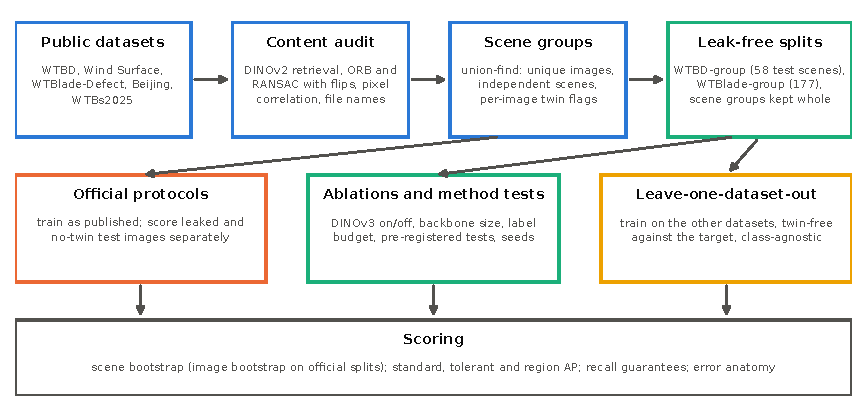
\includegraphics[width=\linewidth]{fig7_pipeline}
\caption{Overview of the study. The content-based audit produces scene groups and per-image twin flags. These define the leak-free splits (WTBD-group, WTBlade-group) and the leaked and no-twin subsets of the official test sets. Every experiment shares the same evaluator and scene bootstrap.}
\label{fig:pipeline}
\end{figure}

\subsection{Contributions}
\begin{itemize}
\item \textbf{A leakage audit of the public blade benchmarks} (Table~\ref{tab:audit}, Fig.~\ref{fig:twins}). We find twins for 78\%, 84\% and 92\% of the official test images of WTBD, Wind Surface and WTBlade-Defect. A literature check found no earlier audit of these datasets.
\item \textbf{A reproduction record of BladeYOLO} (Section~\ref{sec:history}, Fig.~\ref{fig:official-bladeyolo}). It explains why our reproduction gave different results: an unpublished split, a public copy with 220 fewer images, our own early code defects, and leakage.
\item \textbf{The size of the inflation}, measured with one detector and recipe. We compare leaked against no-twin test images (Table~\ref{tab:subsets}) and official against scene-grouped splits (Table~\ref{tab:split-only}). We also show that tuning on the official splits selects for memorisation (Table~\ref{tab:tuning}).
\item \textbf{Two leak-free benchmarks}, WTBD-group and WTBlade-group, with audited splits, scene groups, a scene bootstrap and baselines for four detector families (Table~\ref{tab:leakfree}).
\item \textbf{Controlled ablations} that attribute the advantage of a DINOv3-fused YOLO to the frozen features alone, across the learning curve and three backbone sizes (Tables~\ref{tab:ablation}, \ref{tab:backbone}).
\item \textbf{RF-DETR-FP}, a detection transformer with a frozen DINOv3 prior beside its fine-tuned encoder, motivated by measured feature drift and encoder collapse. It was tested under a pre-registered paired protocol on leak-free and official splits (Section~\ref{sec:fp-results}).
\item \textbf{Measured ceilings}: annotator self-consistency, box granularity, subset luck and error anatomy (Section~\ref{sec:why}).
\item \textbf{A leave-one-dataset-out test} with twin-free pools (Section~\ref{sec:lodo}), and \textbf{a recall-guarantee failure} caused by leaked calibration (Table~\ref{tab:conformal}).
\item \textbf{A ledger of the method tests} we ran or formally gated, including the failures (Table~\ref{tab:ledger}).
\end{itemize}

The authors of the papers we discuss followed common practice, which is to augment and then split at random. Our argument is about the protocol, not about them. We cannot say that any specific published number is due to memorisation, because those splits were not published.

\subsection{Organisation}
Section~\ref{sec:related} reviews related work. Section~\ref{sec:audit} presents the datasets and the leakage audit, and Section~\ref{sec:benchmarks} the leak-free benchmarks and the evaluation protocol. Section~\ref{sec:models} describes the detectors, including the proposed RF-DETR-FP. Section~\ref{sec:official} reports the official protocols: the reproduction of BladeYOLO, our scores against the published ones and what those scores are made of. Section~\ref{sec:leakfree} gives the leak-free results and ablations, and Section~\ref{sec:why} explains why leak-free scores are low. Section~\ref{sec:lodo} tests whether external data replaces target labels, and Section~\ref{sec:failed} records what did not work. Section~\ref{sec:discussion} closes with recommendations, limitations and conclusions. The appendices give the project timeline (Appendix~\ref{app:timeline}), the conclusions we corrected along the way (Appendix~\ref{app:corrections}), the engineering defects that affected results (Appendix~\ref{app:engineering}) and the per-class audit and full run registry (Appendix~\ref{app:registry}).

\section{Related Work}
\label{sec:related}

\subsection{Blade Defect Detection}
Early deep-learning work on blade imagery used transfer learning and ensembles on classified crops~\cite{yangblade}. Detection on UAV imagery started with the DTU NordTank inspection set~\cite{shihavuddin,dtudata} and drone-footage detectors~\cite{foster}. Most recent work adapts single-stage YOLO detectors~\cite{yolo,yolov4,ultralytics,yolov12} with task-specific modules. GFD-YOLOX combines global and local attention with multi-feature fusion and introduced the Wind Surface Defect data~\cite{gfdyolox}. GA-YOLOv5 tunes 30 hyperparameters by a genetic search and adds Unity-rendered images~\cite{gayolo}. KGP-YOLO first locates the blade with a keypoint network and crops it, then detects with routing attention~\cite{kgpyolo}. BladeYOLO~\cite{bladeyolo} replaces the backbone of YOLOv12-L~\cite{yolov12} with frozen DINOv3 ViT-S/16 features~\cite{dinov3}. It adds Fourier-amplitude style injection, a wavelet-convolution detail branch~\cite{wtconv} and Cross-Mamba guidance~\cite{mamba,vmamba}, and it is close in spirit to DINO-YOLO in civil engineering~\cite{dinoyolo}. Data-descriptor papers have added WTBD~\cite{wtbd} and WTBs2025~\cite{wtbs2025}, and WTBlade-Defect is distributed through Roboflow Universe~\cite{fengche}. Training-free inspection with knowledge-augmented vision--language models~\cite{seeingunseen} and box-to-mask supervision with SAM~\cite{boxes2pixels,sam} are recent directions. We have not tested those specific claims on a leak-free split.

\subsection{Detection Architectures and Foundation Features}
Two-stage detectors with region proposals~\cite{fasterrcnn} and feature pyramids~\cite{fpn} gave way, for real-time use, to dense single-stage detectors trained with focal or IoU-based losses~\cite{focal,giou,diou,wiou}. DETR~\cite{detr} casts detection as set prediction with Hungarian matching~\cite{hungarian}. Deformable DETR~\cite{deformabledetr} and DINO~\cite{dinodetr} made it trainable at scale, and RT-DETR~\cite{rtdetr}, D-FINE~\cite{dfine} and LW-DETR~\cite{lwdetr} made it real-time. RF-DETR~\cite{rfdetr} builds on LW-DETR with a windowed DINOv2~\cite{dinov2} ViT~\cite{vit} encoder, searched by neural architecture search. It is strong on the multi-domain Roboflow100-VL benchmark~\cite{rf100vl}, which makes it a natural generic baseline for a niche industrial domain. DINOv3~\cite{dinov3} offers frozen dense features of high quality. DEIMv2~\cite{deimv2} uses DINOv3 backbones inside a real-time DETR, and F-VLM~\cite{fvlm} detects on top of frozen vision--language features. Fine-tuning can distort pretrained features and underperform out of distribution~\cite{lpft}. Adapting foundation features to a new setting, for example by 3D-aware fine-tuning~\cite{fit3d} or continued self-supervision~\cite{data2vec}, is an alternative; our encoder-adaptation arm (G27 D1) collapsed instead, which motivates keeping one encoder frozen, as we do in RF-DETR-FP. Open-vocabulary detectors such as OWLv2~\cite{owlv2} and Grounding DINO~\cite{groundingdino} promise detection without labels; we test OWLv2 on blades.

\subsection{Leakage, Near-Duplicates and Benchmark Validity}
Near-duplicates between training and test data are documented for CIFAR~\cite{barz} and for geospatial mapping data~\cite{adimoolam}. More broadly, leakage is a source of irreproducible machine-learning results across sciences~\cite{kapoor}. A freshly collected test set can show lower accuracy than a reused one~\cite{recht}, and label errors in test sets can reorder benchmark rankings~\cite{northcutt}. Long-tail memorisation is a mechanism by which rare test examples are classified correctly through similar training examples~\cite{feldman}. We apply this line of work to blade defect benchmarks. We add a same-detector measurement of what the leak buys, and show that tuning on a leaky benchmark rewards it.

\subsection{Label Noise and Granularity in Evaluation}
TedEval~\cite{tedeval} handles split and merged instances in text detection. Box-annotation noise has been studied in detection evaluation~\cite{murrugarra}, in repeated labels~\cite{tschirschwitz}, in multiple-instance training under inaccurate boxes~\cite{oamil} and through box-uncertainty regression~\cite{klloss}. TIDE~\cite{tide} decomposes detection errors by type. We measure the same kind of ambiguity from accidental repeated labels: independently annotated copies of the same image.

\subsection{Calibration, Low-Label Learning and Data Selection}
Conformal prediction~\cite{vovk} and conformal risk control~\cite{crc} give distribution-free guarantees under exchangeability, and both have been applied to detection~\cite{andeol}. Few-shot detection results vary strongly with the sampled shots~\cite{tfa}, and novel objects often receive good boxes with low scores~\cite{attentionrpn}. Teacher--student semi-supervised detection~\cite{meanteacher,unbiasedteacher,softteacher} and point supervision~\cite{pointdetr} reduce labelling cost. Cold-start selection uses core sets~\cite{coreset}, typicality~\cite{typiclust}, coverage~\cite{probcover} or self-supervised patch features~\cite{freesel}. Datamodels~\cite{datamodels} study how predictions depend on the training subset. Multi-dataset detection with partitioned label spaces~\cite{multidataset} and training-domain model selection~\cite{domainbed} inform our leave-one-dataset-out design. Copy-paste~\cite{copypaste} is a known augmentation, and masked feature distillation~\cite{data2vec} a known self-supervised objective. We test both only as recipe components.

\section{Datasets and the Leakage Audit}
\label{sec:audit}

\subsection{Datasets}
We use each dataset's official classes, because the taxonomies conflict across datasets (Section~\ref{sec:filecounts}). Fig.~\ref{fig:gallery} shows random labelled examples, and Table~\ref{tab:audit} summarises the audit.

\begin{itemize}
\item \textbf{WTBD}~\cite{wtbd}: 1{,}065 drone images of six classes (craze, corrosion, surface\_injure, thunderstrike, crack, hide\_craze). It was double-annotated with a reported Cohen's $\kappa=0.897$, and its official split is random (seed 42).
\item \textbf{Wind Surface Defect}~\cite{gfdyolox}, used by BladeYOLO: 3{,}570 files in our public copy against the 3{,}790 the BladeYOLO paper reports. Five classes: corrosion, dirt, hide\_craze, surface\_eye, thunderstrike.
\item \textbf{WTBlade-Defect} (fengChe)~\cite{fengche}, used by BladeYOLO: 10{,}660 Roboflow-exported frames of seven classes (burn, crack, deformity, dirt, oil, peeling, rust).
\item \textbf{Auxiliary sources} used only for the leave-one-dataset-out pools and the audit: WTBs2025~\cite{wtbs2025}, two Beijing Roboflow exports, the DTU NordTank imagery~\cite{dtudata} and drone-footage tiles~\cite{foster}.
\end{itemize}

\begin{figure*}[!t]
\centering
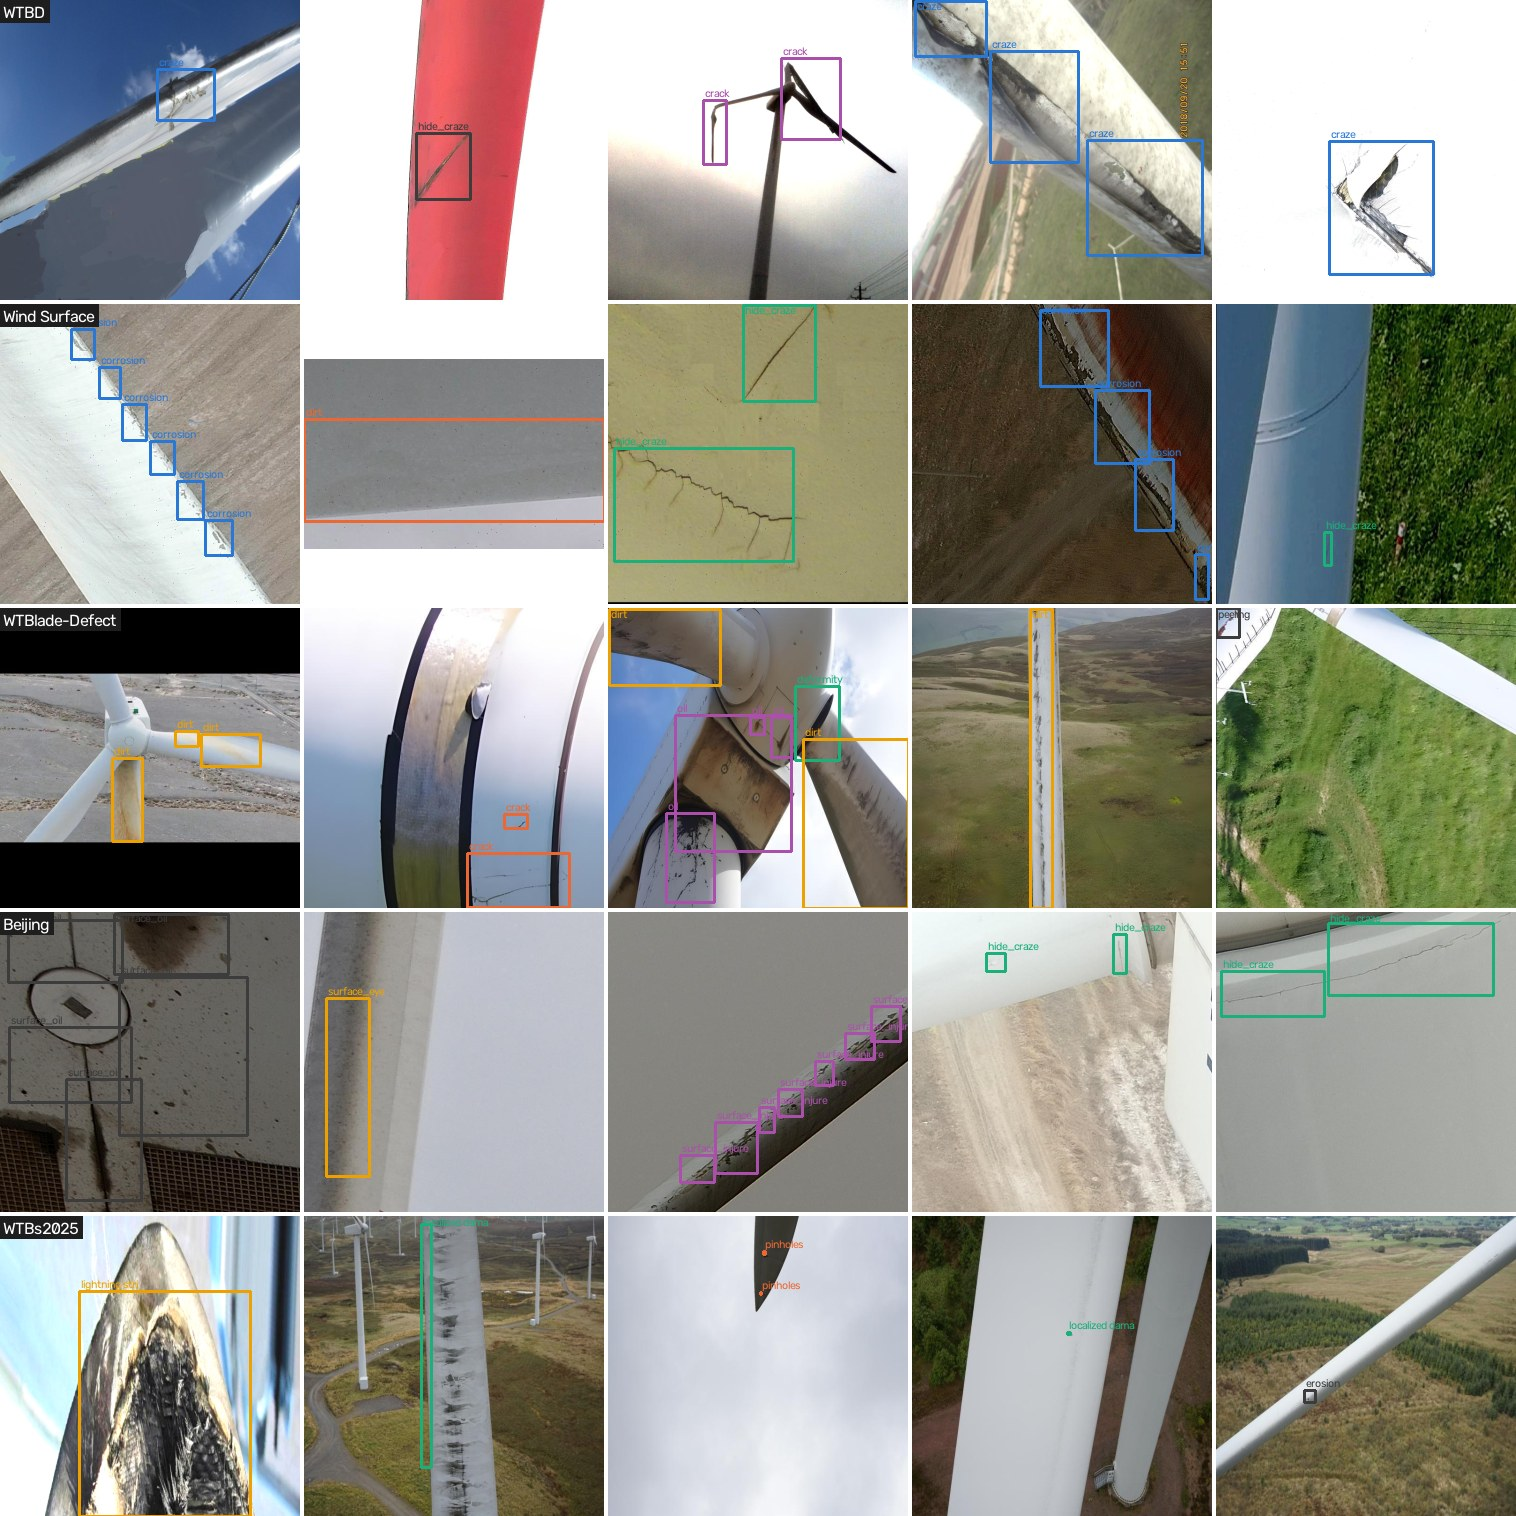
\includegraphics[width=0.86\textwidth]{fig8_dataset_gallery}
\caption{Random labelled training images from each dataset (fixed seed; the first three in each row are required to show a class not yet shown). Colour marks the class within a row. Note the differences in viewpoint and box style, from close-ups with one box (WTBD) to chains of small boxes along an edge (Wind Surface, Beijing) and very small boxes (WTBs2025). Black squares in WTBlade-Defect are the Roboflow export's offline cutout augmentation.}
\label{fig:gallery}
\end{figure*}

\begin{table*}[!t]
\centering
\caption{The three benchmarks and their official splits. Unique images and scenes come from the content-based audit. A \emph{twin} is a near-copy or same-scene image among the images the run trained on.}
\label{tab:audit}
\footnotesize
\begin{tabularx}{\textwidth}{@{}p{0.11\textwidth} r r r p{0.12\textwidth} p{0.2\textwidth} X@{}}
\toprule
Dataset & Files & Unique & Scenes & Official split (train/val/test) & Test images with a training twin & How the twin arises \\
\midrule
WTBD~\cite{wtbd} & 1{,}065 & 597 & $\sim$550 & 745/159/161 & \textbf{125/161 (78\%)} & Duplicate and augmented copies of one photograph, split at random (seed 42) \\
Wind Surface~\cite{gfdyolox} & 3{,}570 & 954 & \textbf{81} & 2{,}856/714 (val\,=\,test) & \textbf{600/714 (84\%)} pixel twins ($r\geq0.99$) & 1{,}785 originals plus one augmented copy each (550 pairs split across train and val); up to 44 tiles per drone photograph (386 of 882 photographs on both sides) \\
WTBlade-Defect~\cite{fengche} & 10{,}660 & 1{,}146 & 803 & 9{,}010/1{,}097/553 & \textbf{499/542 (92\%)} same scene; \textbf{360 (66\%)} copies of a training frame & About three Roboflow augmentation copies per source frame; consecutive drone-video frames \\
\bottomrule
\end{tabularx}
\end{table*}

\subsection{Audit Method}
Files cannot be compared by name or hash, because the copies are flipped, rotated, recoloured or re-encoded. We therefore combine five signals (Algorithm~\ref{alg:audit}):
\begin{enumerate}
\item \textbf{Retrieval:} DINOv2~\cite{dinov2} image embeddings and cosine nearest neighbours.
\item \textbf{Geometric verification:} flip-aware ORB~\cite{orb} keypoint matching with a RANSAC~\cite{ransac} similarity transform; a pair is verified with at least 25 inliers.
\item \textbf{Pixel twins:} the maximum Pearson correlation at $48\times48$ px over the eight flips and quarter-turn rotations; a twin has $r\geq 0.99$.
\item \textbf{Provenance from file names:} Roboflow source prefixes, \texttt{DJI\_xxxx\_r\_c} tile coordinates, and \texttt{\_0}/\texttt{\_1} augmentation pairs.
\item \textbf{Grouping:} union-find over all of the above, with DINOv2 cosine $\geq 0.93$ counted as the same scene. Deduplication is non-chaining, so that a chain of weak matches cannot merge unrelated images.
\end{enumerate}

\begin{algorithm}[!t]
\caption{Content-based twin and scene audit}
\label{alg:audit}
\footnotesize
\begin{algorithmic}[1]
\Require images $\mathcal{I}$, file names, thresholds $\tau_{\cos}=0.93$, $n_{\mathrm{inl}}=25$, $\tau_{r}=0.99$
\State $e_i \gets \mathrm{DINOv2}(i)/\lVert\cdot\rVert$ for all $i\in\mathcal{I}$
\State $\mathcal{U} \gets$ union-find over $\mathcal{I}$
\For{each $i$ and its $k$ nearest neighbours $j$ by $e_i^\top e_j$}
  \If{$e_i^\top e_j \geq \tau_{\cos}$} \textsc{Union}$(i,j)$ \Comment{same scene}
  \EndIf
  \If{$\max_{g\in D_4}\#\mathrm{inliers}(\mathrm{ORB}(i), \mathrm{ORB}(g(j))) \geq n_{\mathrm{inl}}$} \textsc{Union}$(i,j)$
  \EndIf
  \If{$\max_{g\in D_4} r(i_{48}, g(j)_{48}) \geq \tau_r$} \textsc{Union}$(i,j)$; mark pixel twin
  \EndIf
\EndFor
\State \textsc{Union} images sharing a source prefix, a parent photograph (tile name) or an \texttt{\_0}/\texttt{\_1} stem
\State flag test image $t$ as \emph{leaked} if its group contains an image the run trained on
\State \Return groups (scenes), per-image flags
\end{algorithmic}
\end{algorithm}

Example sheets were checked by eye for every dataset and every outcome. On Wind Surface, the first pixel comparison (flips only) found 532 of 714 validation images (75\%). Adding rotations and restricting the comparison to the images actually trained on gives 600 (84\%). The Wind Surface ``no-twin'' subset has no near-identical copy in training. Most of it, however, comes from drone photographs with other tiles in training, so it is cleaner rather than leak-free. Fig.~\ref{fig:twins} shows test images and their training twins, drawn at random.

\begin{figure*}[!t]
\centering
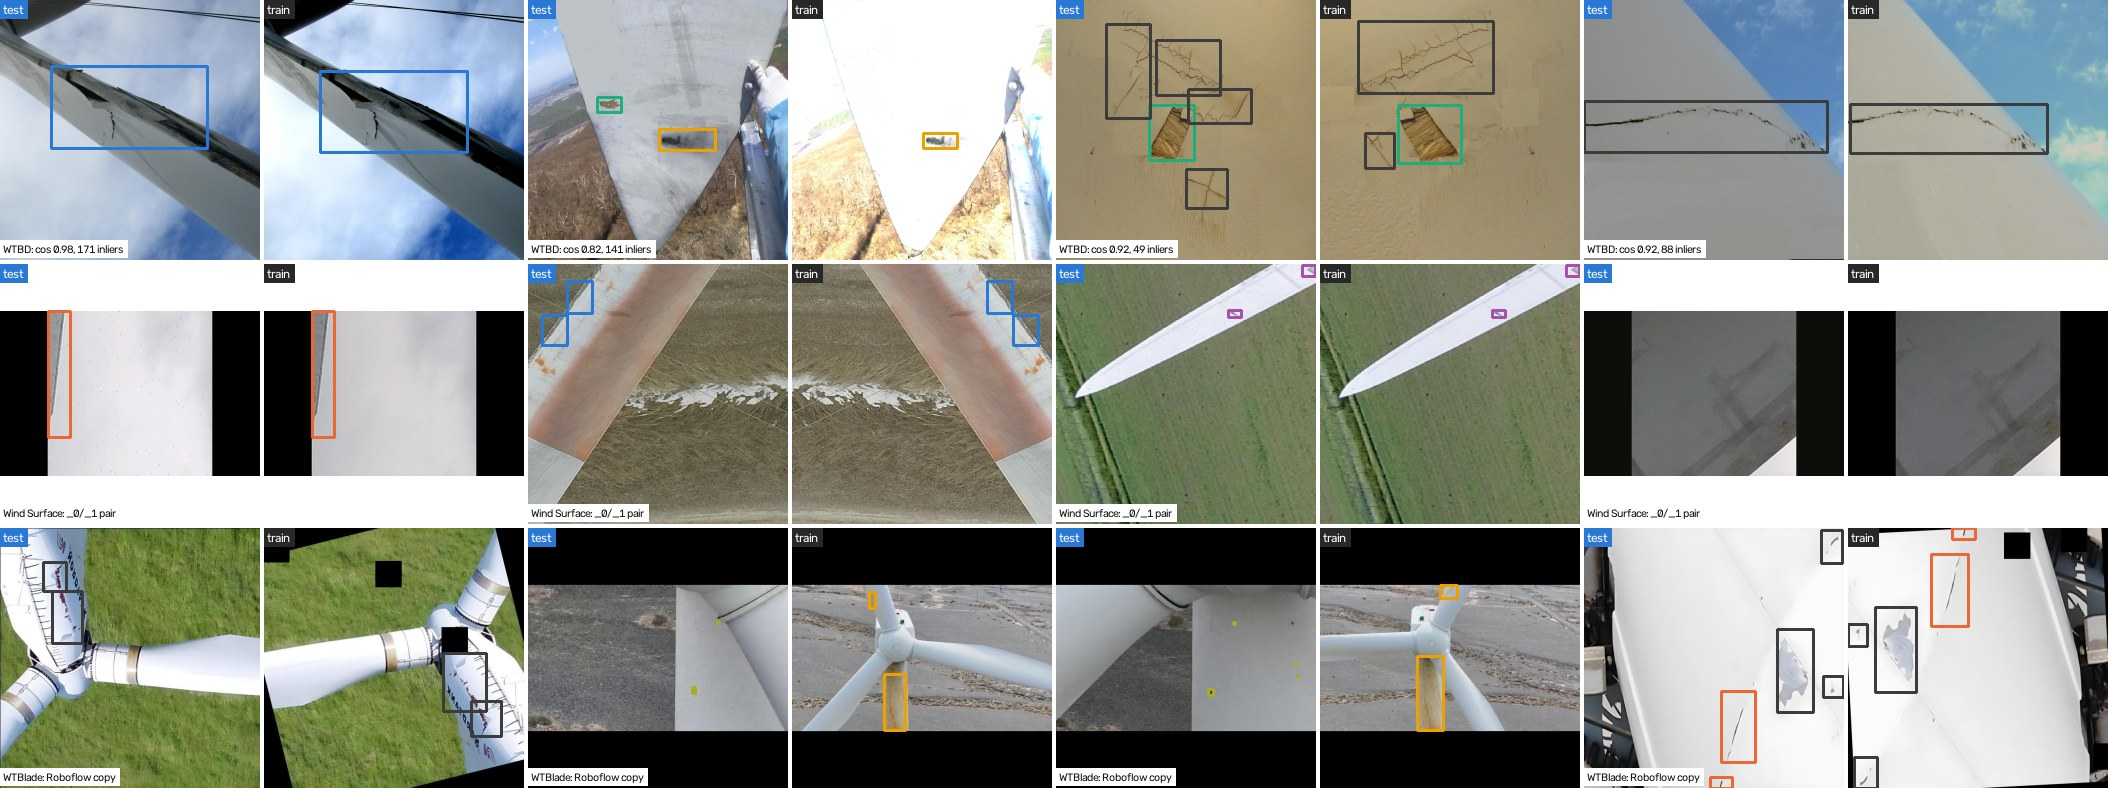
\includegraphics[width=\textwidth]{fig10_twins}
\caption{Official test images (blue tag) next to their training twins (black tag), drawn at random with a fixed seed from the leaked subsets. Labels are drawn as supplied. Row 1: WTBD, with DINOv2 cosine and ORB inliers. Row 2: Wind Surface \texttt{\_0}/\texttt{\_1} pairs split across the partition. Row 3: WTBlade-Defect Roboflow copies of one source frame.}
\label{fig:twins}
\end{figure*}

\subsection{What the File Counts Hide}
\label{sec:filecounts}
File count is a poor guide to the information a dataset holds (Fig.~\ref{fig:size}). Wind Surface's 3{,}570 files come from about 81 independent scenes. All its \texttt{surface\_eye} boxes (412 in the raw files, 103 after deduplication) come from tiles of a single photograph. Any \texttt{surface\_eye} score on the original split, including published ones, was therefore measured on tiles of a training photograph. WTBD has far fewer files and far more independent scenes per class. Three more findings limit what can be merged:
\begin{itemize}
\item \textbf{Same-named classes do not match across datasets.} Mutual crop retrieval between same-named classes is at most 0.33, apart from the two Beijing exports, which are the same data.
\item \textbf{Datasets overlap under other names.} WTBs2025 shares 1{,}499 images with WTBlade-Defect under different class names (peeling becomes erosion). The Beijing exports contain WTBD test photographs.
\item \textbf{Licences are not what the export pages say.} ``NORDTANK'' is legible on many WTBlade-Defect nacelles, so the set contains DTU imagery~\cite{shihavuddin,dtudata}, which is CC BY-NC, while its Roboflow page states CC BY 4.0. It also contains synthetic copy-paste images.
\end{itemize}

\begin{figure}[!t]
\centering
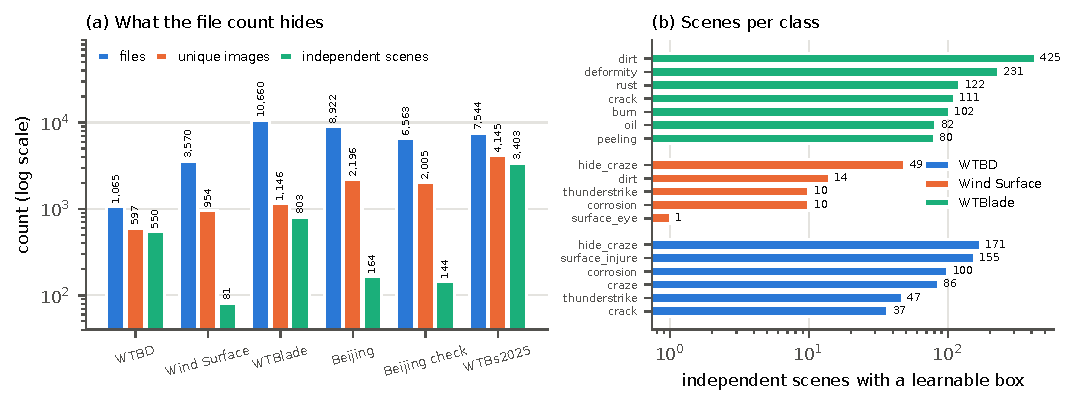
\includegraphics[width=\linewidth]{fig9_effective_size}
\caption{Effective dataset size. (a) Files, unique images and independent scenes per dataset. (b) Independent scenes with a learnable box, per class. A single scene supports Wind Surface's \texttt{surface\_eye}.}
\label{fig:size}
\end{figure}

\subsection{Protocols of Published Work}
The augment-then-split pattern is not specific to one paper (Table~\ref{tab:protocols}). KGP-YOLO expands 130 DTU images to 780 and then splits them 624/78/78~\cite{kgpyolo}. GA-YOLOv5 adds CLAHE copies and uses a random 60/40 split of repeated shots of one turbine~\cite{gayolo}. BladeYOLO's WTBlade numbers use its authors' own 9:1 re-split of 5{,}326 images, which is not public~\cite{bladeyolo}.

\begin{table}[!t]
\centering
\caption{Evaluation protocols of published blade-defect detectors, as read from the papers.}
\label{tab:protocols}
\footnotesize
\begin{tabularx}{\linewidth}{@{}l X@{}}
\toprule
Work & Protocol \\
\midrule
GFD-YOLOX~\cite{gfdyolox} & Wind Surface: 1{,}785 originals plus augmented copies, random split; tiles of one photograph on both sides \\
BladeYOLO~\cite{bladeyolo} & Wind Surface random 4:1 (3{,}790 images, no list); WTBlade 9:1 re-split of 5{,}326 images (not public); no separate validation set; random label fractions \\
KGP-YOLO~\cite{kgpyolo} & Augment (flips, brightness, saturation) before the split; DTU 130 $\rightarrow$ 780 images, 624/78/78; single runs \\
GA-YOLOv5~\cite{gayolo} & 432 DTU images doubled by CLAHE, random 60/40 split of repeated shots of one turbine; best synthetic amount read off the test set \\
WTBD~\cite{wtbd} & Random split, seed 42; no detection baselines \\
\bottomrule
\end{tabularx}
\end{table}

\section{Leak-Free Benchmarks and Evaluation Protocol}
\label{sec:benchmarks}

\subsection{Splits}
\textbf{WTBD-group.} The 1{,}065 WTBD images are split by scene into 745/159/161 images, the official sizes. The split holds 1{,}109/240/235 boxes and 224/60/58 scene groups. It was audited until no held-out image matched the training set under DINOv2 and ORB verification. The 25\% and 50\% label fractions are nested subsets of the training scenes.

\textbf{WTBlade-group.} We start from 10{,}527 WTBlade-Defect images, leaving out the 133 that match WTBD so that the two benchmarks share nothing. From them we form 841 groups out of 2{,}791 source frames, verified pairs and DINOv2 neighbours. A class-stratified 70/15/15 split over groups converged with no held-out-to-train match after 11 rounds of the audit. We keep one image per source frame, giving 2{,}136/323/332 frames, 5{,}237/729/748 boxes and 177 test scenes, with all seven classes in every split.

\textbf{A residual leak in our own splits.} While building a later pool, we added the pixel test to our audit and ran it on these splits. It found copies that DINOv2 and ORB had missed: 6 of 161 test and 6 of 159 validation images on WTBD-group, and 1 of 332 and 1 of 323 on WTBlade-group (Fig.~\ref{fig:residual}). All six WTBD-group test pairs are real copies by eye, re-exposed, darkened, tinted or rotated. We rescored 116 cached WTBD-group runs without those images. This changes \mcoco by $-0.62$ on average (range $-1.09$ to $+0.33$) and \mfifty by $-0.70$; 20 WTBlade-group runs change by $\pm0.03$. Our leak-free numbers are therefore inflated by under a point. We kept the splits unchanged, so that every comparison stays like for like, and we report every pre-registered decision both ways. None changes. A leak-free split needs the pixel test next to scene grouping, and ``audited'' is only as good as the audit.

\begin{figure}[!t]
\centering
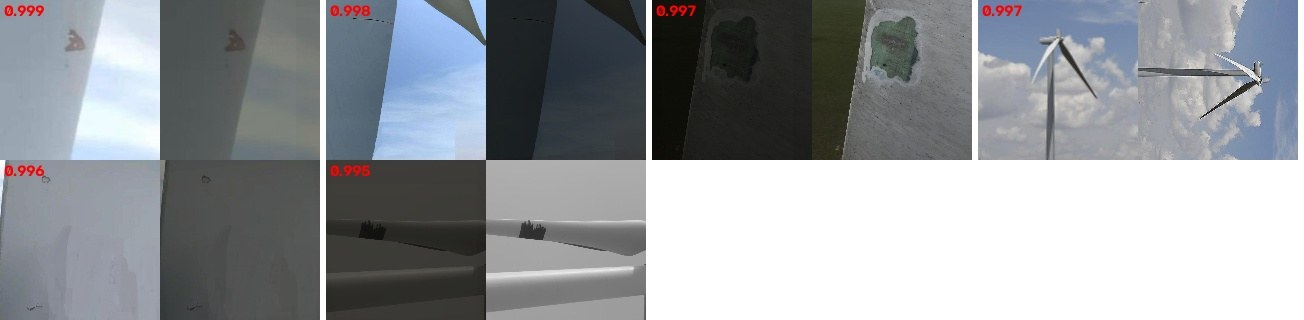
\includegraphics[width=\linewidth]{fig28_residual_twins}
\caption{The residual leak in our WTBD-group test set: each pair is a test image and its pixel twin in train, with the correlation. Photometric copies defeat DINOv2 + ORB grouping.}
\label{fig:residual}
\end{figure}

\subsection{Selection and Reporting}
Model selection uses validation only, and results are reported on test, scored once. Wind Surface has no separate test split, so we carve a seeded 10\% of its training set for validation (2{,}570/286/714). Unless stated otherwise, ``points'' are percentage points of AP.

\subsection{Evaluator}
We use a 101-point COCO-style evaluator~\cite{coco,pascal} (\texttt{tools/bootstrap\_ci.py}). On identical predictions it agrees with Ultralytics' \texttt{ap\_per\_class}~\cite{ultralytics} within 0.4 points on every run and subset, so the gaps to published figures are not an artefact of the metric. Ultralytics' \texttt{val} reports differ by 1--2.5 points from cached predictions, because of its rectangular-batch inference path. Tables state which evaluator they use.

\subsection{Scene Bootstrap}
Test images of one scene are correlated, so intervals that resample images are too narrow~\cite{fieldwelsh}. Let $\mathcal{G}=\{g_1,\dots,g_S\}$ be the test scene groups. A replicate draws $S$ groups with replacement, $\mathcal{G}^{*b}$, and recomputes the metric on the union of their images. For a paired comparison between models $A$ and $B$ that both predicted every test image,
\begin{equation}
\Delta^{*b} = M_A\!\left(\textstyle\bigcup_{g\in\mathcal{G}^{*b}} g\right) - M_B\!\left(\textstyle\bigcup_{g\in\mathcal{G}^{*b}} g\right),
\label{eq:bootstrap}
\end{equation}
with the same draw used for both models. We report the 2.5 and 97.5 percentiles of $\{\Delta^{*b}\}_{b=1}^{2000}$ and $P(\Delta>0)=\frac{1}{B}\sum_b\mathbb{1}[\Delta^{*b}>0]$~\cite{efron}. With two training seeds, $\Delta$ is the mean over seeds within each replicate. With two datasets, the dataset mean is taken within each replicate, with independent draws per dataset. The official splits have no scene groups, so their intervals resample images and are therefore narrower than they should be.

\subsection{Three Box Scores}
\textit{Standard} AP uses one-to-one matching at IoU~$\geq 0.5$ (\apfifty) or averaged over IoU 0.50:0.95 (\mcoco). \textit{Tolerant} AP lets one prediction match several same-class labels whose union it fits, and ignores fragments of an already found defect. \textit{Region} AP is the pixel-level precision and recall of the union of predicted boxes against the union of labels, on a 4-px grid. For a class $c$ at confidence threshold $\theta$,
\begin{equation}
P_c(\theta)=\frac{|\,\cup\hat{B}_c(\theta)\cap\cup B_c\,|}{|\,\cup\hat{B}_c(\theta)\,|},\quad
R_c(\theta)=\frac{|\,\cup\hat{B}_c(\theta)\cap\cup B_c\,|}{|\,\cup B_c\,|},
\label{eq:region}
\end{equation}
and region AP is the area under $(R_c,P_c)$. It does not depend on how a defect is cut into boxes. A trivial detector that boxes the whole image scores 14--24 region AP on our benchmarks, so raw region AP must be read against that floor.

\subsection{Pre-Registration}
From late October onwards, hypotheses were written down with their pass bars before any run or computation, and committed to the repository~\cite{prereg,repo}. A typical primary claim reads: ``the paired difference is $>0$ on each dataset, and the dataset mean has $P(\Delta>0)\geq0.95$''. After a bad result we allow one scope check, on whether any part is usable, and then discard the hypothesis without rescue runs. Post hoc analyses are labelled as such throughout.

\section{Detectors}
\label{sec:models}

We compare four detector families under shared splits, evaluator and bootstrap. Table~\ref{tab:recipes} lists the training settings.

\subsection{YOLO12-L}
The stock Ultralytics YOLO12-L~\cite{ultralytics,yolov12} is COCO-pretrained and uses the CIoU loss~\cite{diou} and AdamW~\cite{adamw} (learning rate 0.001, weight decay 0.01) with a cosine schedule~\cite{sgdr}. Training uses mosaic~\cite{yolov4}, vertical and horizontal flips and random quarter turns. A quarter turn maps an axis-aligned box onto an exactly tight box, and drone views have no canonical ``up''.

\subsection{BladeYOLO-v2}
\label{sec:byv2}
BladeYOLO-v2 is our re-engineering of the BladeYOLO idea after a code audit (Section~\ref{sec:history}). It keeps the COCO-pretrained YOLOv12-L backbone, neck and head, so that 1{,}239 pretrained tensors transfer, and adds BladeYOLO's ingredients as zero-initialised residual branches (Fig.~\ref{fig:arch-byv2}). Training therefore starts exactly at the pretrained detector, and it learns how much of each addition to use:
\begin{itemize}
\item \textbf{DinoFuse.} Frozen DINOv3 features~\cite{dinov3} from blocks 4, 8 and 12 (ViT-S/16 by default; ViT-B/16 and ViT-L/16 in the ablations) are resized to the P3, P4 and P5 backbone levels. They are projected there and added through a zero-initialised $1\times1$ convolution: $X_\ell' = X_\ell + W_\ell\,\phi(\mathrm{Resize}(D_{b(\ell)}))$ with $W_\ell=0$ at initialisation.
\item \textbf{Deformable refinement} of the P3 and P4 neck outputs with modulated deformable convolution (DCNv2~\cite{dcnv2}), for irregular contours such as cracks and erosion edges. Offsets start at zero and modulation at 0.5.
\item \textbf{Selective-scan refinement} of the P5 neck output: a four-direction VMamba-style scan~\cite{vmamba,mamba} in the chunked Mamba-2 form, written in plain PyTorch. It matches a step-by-step reference recurrence to $1.8\times10^{-14}$.
\item \textbf{WIoU v3}~\cite{wiou} box loss in place of CIoU. The assigner keeps CIoU.
\end{itemize}
With ViT-S/16 the model has 53.7\,M parameters (32.1\,M trainable) and 233.5 GFLOPs. Deformable and selective-scan blocks run in fp32 under mixed precision~\cite{mixedprecision}, and YOLOv12's area-attention scores are computed in fp32. Without these changes, fp16 overflows produced NaNs at epochs 9, 17 and 99--149 (Appendix~\ref{app:engineering}).

\begin{figure*}[!t]
\centering
\resizebox{0.92\textwidth}{!}{% BladeYOLO-v2 (models/bladeyolo2-l.yaml; models/dino_fusion.py, morphology.py, ss2d.py, wiou.py)
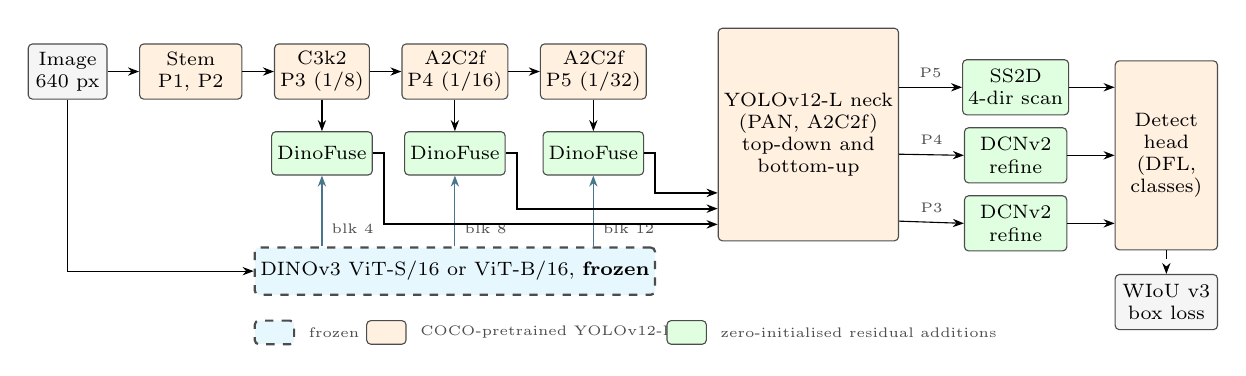
\begin{tikzpicture}[
  font=\scriptsize, >={Stealth[length=4pt]}, node distance=3mm and 4mm,
  blk/.style={draw=black!70, rounded corners=1.5pt, align=center, minimum height=7mm, inner sep=2pt, fill=#1},
  blk/.default=white,
  lab/.style={font=\tiny, text=black!70, align=center},
  frozen/.style={blk=cyan!10, dashed, thick},
  coco/.style={blk=orange!12},
  new/.style={blk=green!12},
]
% backbone row
\node[blk=gray!8, minimum width=10mm] (img) {Image\\640 px};
\node[coco, right=of img, minimum width=13mm] (s1) {Stem\\P1, P2};
\node[coco, right=of s1, minimum width=11mm] (p3) {C3k2\\P3 (1/8)};
\node[coco, right=of p3, minimum width=11mm] (p4) {A2C2f\\P4 (1/16)};
\node[coco, right=of p4, minimum width=11mm] (p5) {A2C2f\\P5 (1/32)};
\draw[->] (img) -- (s1); \draw[->] (s1) -- (p3); \draw[->] (p3) -- (p4); \draw[->] (p4) -- (p5);
% DINOv3 and fusion
\foreach \k in {3,4,5} {
  \node[new, below=4mm of p\k, minimum width=11mm, minimum height=5.5mm] (f\k) {DinoFuse};
  \draw[->] (p\k) -- (f\k);
}
\node[frozen, below=9mm of f4, minimum height=6mm] (dino) {DINOv3 ViT-S/16 or ViT-B/16, \textbf{frozen}};
\draw[->] (img) |- (dino.west);
\foreach \k/\b in {3/4, 4/8, 5/12} {
  \draw[->, cyan!50!black] (dino.north -| f\k) -- node[right, lab, pos=0.25]{blk \b} (f\k.south);
}
% neck
\node[coco, right=9mm of p5, minimum width=19mm, minimum height=27mm, yshift=-8mm] (neck) {YOLOv12-L neck\\(PAN, A2C2f)\\top-down and\\bottom-up};
\foreach \k/\d in {5/2.2, 4/4.2, 3/6.2} {
  \draw[->, thick] (f\k.east) -- ++(1.4mm,0) |- ([yshift=-\d mm]f5.south -| neck.west);
}
% refinements after the neck
\node[new, right=8mm of neck, minimum width=13mm, yshift=6mm] (r5) {SS2D\\4-dir scan};
\node[new, below=1.5mm of r5, minimum width=13mm] (r4) {DCNv2\\refine};
\node[new, below=1.5mm of r4, minimum width=13mm] (r3) {DCNv2\\refine};
\draw[->] ([yshift=6mm]neck.east) -- node[above, lab]{P5} (r5.west);
\draw[->] ([yshift=-2.5mm]neck.east) -- node[above, lab]{P4} (r4.west);
\draw[->] ([yshift=-11mm]neck.east) -- node[above, lab]{P3} (r3.west);
\node[coco, right=6mm of r4, minimum width=13mm, minimum height=24mm] (head) {Detect\\head\\(DFL,\\classes)};
\foreach \k in {3,4,5} {\draw[->] (r\k.east) -- (r\k.east -| head.west);}
\node[blk=gray!8, below=3mm of head, minimum width=13mm] (loss) {WIoU v3\\box loss};
\draw[->, dashed] (head) -- (loss);
% legend
\node[frozen, minimum height=3mm, minimum width=5mm, below=3mm of dino.south west, anchor=north west] (l1) {};
\node[right=0.5mm of l1, lab, anchor=west] {frozen};
\node[coco, minimum height=3mm, minimum width=5mm, right=9mm of l1] (l2) {};
\node[right=0.5mm of l2, lab, anchor=west] {COCO-pretrained YOLOv12-L};
\node[new, minimum height=3mm, minimum width=5mm, right=33mm of l2] (l3) {};
\node[right=0.5mm of l3, lab, anchor=west] {zero-initialised residual additions};
\end{tikzpicture}
}
\caption{BladeYOLO-v2. A COCO-pretrained YOLOv12-L with three kinds of zero-initialised residual additions: frozen DINOv3 features fused into the backbone levels P3--P5 (DinoFuse), DCNv2 refinement of the P3/P4 neck outputs, and a four-direction selective scan (SS2D) on the P5 neck output. The box loss is WIoU v3. At initialisation the network computes exactly the pretrained YOLOv12-L. Section~\ref{sec:ablation} shows that the frozen DINOv3 features carry its entire advantage.}
\label{fig:arch-byv2}
\end{figure*}

\subsection{RF-DETR}
RF-DETR-M~\cite{rfdetr} (\texttt{rfdetr} 1.11.2) builds on LW-DETR~\cite{lwdetr}. It uses a windowed DINOv2-S/16 encoder~\cite{dinov2}, fine-tuned end to end, whose blocks 3, 6, 9 and 12 feed a single-level (P4, stride 16) projector with 256 channels. A two-stage head selects 300 queries from this memory, and four deformable cross-attention decoder layers~\cite{deformabledetr} refine them. Training uses group-DETR one-to-many assignment (13 groups) and IoU-aware BCE classification with GIoU and L1 box losses~\cite{giou}. We fine-tune from the COCO checkpoint with AdamW (base learning rate $10^{-4}$, encoder $1.5\times10^{-4}$ with layer-wise decay 0.8, weight decay $10^{-4}$), gradient clipping at 0.1 and per-batch multi-scale training. The effective batch is 16 (4 $\times$ 4 accumulation). An exponential moving average~\cite{polyak} of the weights (decay 0.993) is evaluated every epoch, and the best EMA checkpoint on validation is kept. RF-DETR's default learning-rate step at epoch 100 never fires in a 100-epoch run, so we use an explicit cosine schedule (``G26 recipe'').

\subsection{RF-DETR-FP: A Frozen Foundation Prior Beside a Fine-Tuned Encoder}
\label{sec:fp}

\textbf{Motivation.} Three findings of this study, each made before RF-DETR-FP was designed, point to the same lever:
\begin{enumerate}
\item Frozen DINOv3 is the one component that ever helped in our YOLO-family ablations. It adds $+3.9$, $+8.8$ and $+9.0$ \mcoco at 25, 50 and 100\% labels, and ViT-B beats ViT-S (Section~\ref{sec:ablation}).
\item RF-DETR lacks what DINOv3 carries. On WTBlade-group, the frozen-DINOv3 ViT-B YOLO beats fine-tuned RF-DETR-M (18.0 against 16.2/16.9). On WTBD, DINOv3 ViT-B box embeddings re-rank RF-DETR's own outputs for a gain (H18, Table~\ref{tab:ledger}), so its ranking deficit is information that DINOv3 holds and RF-DETR does not use.
\item That information cannot simply be written into RF-DETR's encoder. Fine-tuning moves RF-DETR's features away from generic neighbourhoods (G22-O). Further self-supervised adaptation of its encoder halved the effective rank of its last stage (G27 D1, Section~\ref{sec:failed}), and multi-dataset pretraining did not help (D2).
\end{enumerate}
We therefore keep a second, \emph{frozen} encoder beside the fine-tuned one, rather than adapting either (Fig.~\ref{fig:arch-fp}).

\begin{figure*}[!t]
\centering
\resizebox{\textwidth}{!}{% RF-DETR-M with a frozen DINOv3 prior (G29, "FP"). tools/g29_prior.py
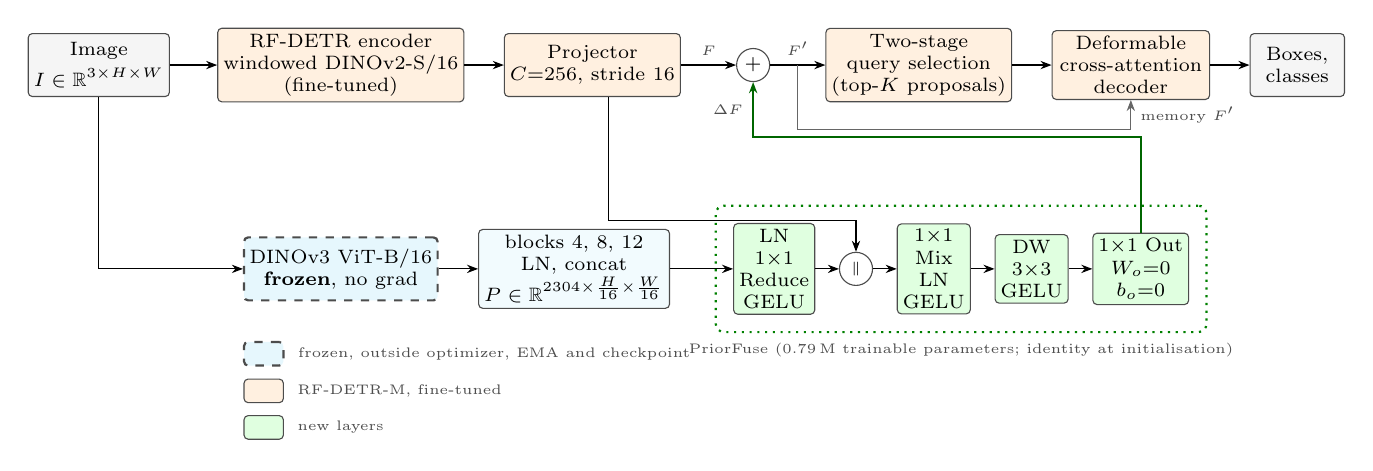
\begin{tikzpicture}[
  font=\scriptsize, >={Stealth[length=4pt]}, node distance=4mm and 5mm,
  blk/.style={draw=black!70, rounded corners=1.5pt, align=center, minimum height=8mm, inner sep=2pt, fill=#1},
  blk/.default=white,
  op/.style={draw=black!70, circle, inner sep=0.5pt, minimum size=4.2mm, fill=white},
  lab/.style={font=\tiny, text=black!70, align=center},
  frozen/.style={blk=cyan!10, dashed, thick},
  train/.style={blk=orange!12},
  new/.style={blk=green!12},
]
% ---------- main RF-DETR path ----------
\node[blk=gray!8, minimum width=12mm] (img) {Image\\[3pt]$I\in\mathbb{R}^{3\times H\times W}$};
\node[train, right=6mm of img, minimum width=22mm] (enc) {RF-DETR encoder\\windowed DINOv2-S/16\\(fine-tuned)};
\node[train, right=of enc, minimum width=15mm] (proj) {Projector\\$C{=}256$, stride 16};
\node[op, right=7mm of proj] (add) {$+$};
\node[train, right=7mm of add, minimum width=20mm] (qs) {Two-stage\\query selection\\(top-$K$ proposals)};
\node[train, right=of qs, minimum width=20mm] (dec) {Deformable\\cross-attention\\decoder};
\node[blk=gray!8, right=of dec, minimum width=12mm] (out) {Boxes,\\classes};
\draw[->] (img) -- (enc);
\draw[->] (enc) -- (proj);
\draw[->] (proj) -- node[above, lab]{$F$} (add);
\draw[->] (add) -- node[above, lab]{$F'$} (qs);
\draw[->] (qs) -- (dec);
\draw[->] (dec) -- (out);
\draw[->, black!60] ($(add.east)!0.5!(qs.west)$) |- ([yshift=-3.5mm]qs.south) -| node[pos=0.75, right, lab]{memory $F'$} (dec.south);

% ---------- frozen prior path ----------
\node[frozen, below=17mm of enc, minimum width=22mm] (dino) {DINOv3 ViT-B/16\\\textbf{frozen}, no grad};
\node[blk=cyan!5, right=of dino, minimum width=15mm] (cat) {blocks 4, 8, 12\\LN, concat\\$P\in\mathbb{R}^{2304\times\frac{H}{16}\times\frac{W}{16}}$};
\draw[->] (img) |- (dino);
\draw[->] (dino) -- (cat);

% ---------- PriorFuse ----------
\node[new, right=8mm of cat, minimum width=9mm] (red) {LN\\$1{\times}1$\\Reduce\\GELU};
\node[op, right=3mm of red] (cc) {\tiny $\Vert$};
\node[new, right=3mm of cc, minimum width=9mm] (mix) {$1{\times}1$\\Mix\\LN\\GELU};
\node[new, right=3mm of mix, minimum width=9mm] (dw) {DW\\$3{\times}3$\\GELU};
\node[new, right=3mm of dw, minimum width=11mm] (o) {$1{\times}1$ Out\\$W_o{=}0$\\$b_o{=}0$};
\draw[->] (cat) -- (red);
\draw[->] (red) -- (cc);
\draw[->] (cc) -- (mix);
\draw[->] (mix) -- (dw);
\draw[->] (dw) -- (o);
\draw[->] (proj.south) ++(2mm,0) |- ([yshift=4mm]cc.north) -- (cc.north);
\draw[->, green!40!black, thick] (o.north) |- ([yshift=-7mm]add.south) -- node[left, lab]{$\Delta F$} (add.south);
\begin{scope}[on background layer]
  \node[draw=green!50!black, dotted, thick, rounded corners=3pt, fit=(red)(cc)(mix)(dw)(o), inner sep=2.2mm,
        label={[lab, anchor=north]south:PriorFuse (0.79\,M trainable parameters; identity at initialisation)}] (pf) {};
\end{scope}
% legend
\node[frozen, minimum height=3mm, minimum width=5mm, below=5mm of dino.south west, anchor=north west] (l1) {};
\node[right=0.5mm of l1, lab, anchor=west] {frozen, outside optimizer, EMA and checkpoint};
\node[train, minimum height=3mm, minimum width=5mm, below=1.5mm of l1] (l2) {};
\node[right=0.5mm of l2, lab, anchor=west] {RF-DETR-M, fine-tuned};
\node[new, minimum height=3mm, minimum width=5mm, below=1.5mm of l2] (l3) {};
\node[right=0.5mm of l3, lab, anchor=west] {new layers};
\end{tikzpicture}
}
\caption{RF-DETR-FP. A frozen DINOv3 ViT-B/16 runs beside RF-DETR-M's fine-tuned windowed DINOv2-S encoder on the same normalised input. Both have patch 16, so the frozen features from blocks 4, 8 and 12 (2{,}304 channels) lie on the projector's grid. PriorFuse adds them to the projector output $F$ before two-stage query selection and decoding. Its output convolution is zero-initialised, so the model at step 0 is exactly RF-DETR-M. DINOv3 sits outside the optimiser, the EMA copy and the checkpoint. Only PriorFuse (0.79\,M parameters) is new.}
\label{fig:arch-fp}
\end{figure*}

\textbf{Architecture.} Let $I\in\mathbb{R}^{3\times H\times W}$ be the ImageNet-normalised input, which is also DINOv3's normalisation. Let $F=\mathrm{Proj}(E_\theta(I))\in\mathbb{R}^{C\times\frac{H}{16}\times\frac{W}{16}}$, with $C=256$, be RF-DETR's projector output. The frozen prior is
\begin{equation}
P=\big[\,\mathrm{LN}(\Phi_4(I));\ \mathrm{LN}(\Phi_8(I));\ \mathrm{LN}(\Phi_{12}(I))\,\big]\in\mathbb{R}^{2304\times\frac{H}{16}\times\frac{W}{16}},
\label{eq:prior}
\end{equation}
where $\Phi_k$ is the patch-token map after block $k$ of DINOv3 ViT-B/16, computed without gradient, and LN is DINOv3's final layer norm~\cite{layernorm}. PriorFuse computes
\begin{align}
S &= \mathrm{GELU}\big(W_r\ast\mathrm{LN}(P)\big), \label{eq:reduce}\\
Z &= \mathrm{GELU}\big(\mathrm{LN}(W_m\ast[F;S])\big), \label{eq:mix}\\
F' &= F + W_o\ast\mathrm{GELU}\big(\mathrm{DW}_{3\times3}(Z)\big),\qquad W_o=0,\ b_o=0\ \text{at}\ t=0, \label{eq:fuse}
\end{align}
where $W_r$ ($2304\rightarrow C$), $W_m$ ($2C\rightarrow C$) and $W_o$ ($C\rightarrow C$) are $1\times1$ convolutions, $\mathrm{DW}_{3\times3}$ is a depthwise convolution~\cite{xception} and GELU is from~\cite{gelu}. $F'$ replaces $F$ as the memory from which the two-stage head selects queries and which the decoder attends to. Because the grids coincide on RF-DETR-M, no resampling is needed. For RF-DETR sizes with other projector levels, $P$ is resized bilinearly.

\textbf{Properties.} (i) At initialisation the patched backbone returns bit-identical features to RF-DETR, which we verify in a unit test at 320 and 768\,px. (ii) The frozen model lives in a process-wide cache, not as a submodule, so it is not in \texttt{parameters()}, the optimiser, the EMA copy or \texttt{state\_dict()}. Checkpoints carry only the 0.79\,M fusion parameters, and gradients reach PriorFuse and never DINOv3, which a unit test also verifies. (iii) The recipe is otherwise unchanged: each FP run uses exactly the arguments of a baseline twin with the same hardware type, so that every comparison is paired. (iv) On a Tesla T4 the frozen ViT-B forward, plus a second job sharing the machine, costs 1.5--1.7$\times$ the baseline's wall time (Table~\ref{tab:recipes}).

\textbf{Novelty, stated plainly.} Fusing frozen foundation features into a detector is prior art: BladeYOLO and DINO-YOLO do it in YOLO~\cite{bladeyolo,dinoyolo}, and DEIMv2 puts DINOv3 in a DETR~\cite{deimv2}. What is specific here is narrower. First, a frozen generic encoder is placed \emph{beside} a fine-tuned one, chosen because of measured evidence that the fine-tuned one drifts from it and collapses when pushed further. Second, the test is leak-aware: we ask whether the gain is still there on images with no training twin. This is a defensible design, not a new module, and we evaluate it as such.

\begin{table*}[!t]
\centering
\caption{Training settings. All RF-DETR runs fine-tune the COCO checkpoint, select the best EMA checkpoint on validation and score test once. Wall times are per run on one Tesla T4 (fp16) unless noted.}
\label{tab:recipes}
\footnotesize
\begin{tabularx}{\textwidth}{@{}l l l l l X@{}}
\toprule
Model & Data & Input & Epochs & Batch & Notes \\
\midrule
YOLO12-L, BladeYOLO-v2 & WTBD-group / WTBD-official & 640 & 150 / 120 & 16 & AdamW 0.001, wd 0.01, cosine, mosaic, flips, Rot90; Ultralytics \\
YOLO12-L, BladeYOLO-v2 ViT-B & WTBlade-group & 640 & 50 & 16 & as above \\
RF-DETR-M (A0) & WTBD-group & 768 & 100 & 4$\times$4 & cosine; 2.5\,h (FP: 4.2\,h) \\
RF-DETR-M (A0) & WTBlade-group & 640 & 60 & 4$\times$4 & cosine; $\approx$3.5\,h (FP: 5.5\,h) \\
RF-DETR-M (G26) & WTBD-official & 768 & 100 & 2$\times$8 & cosine; 3\,h (FP: 4.9\,h) \\
RF-DETR-M (G26) & Wind Surface (2{,}570/286/714) & 640 & 100 & 4$\times$4 & cosine; 7\,h (FP: 10.8\,h) \\
RF-DETR-M (G26) & WTBlade-Defect official & 640 & 40 & 4$\times$4 & cosine; A100 (bf16) \\
RF-DETR-M (V1) & 25\% of WTBD-group, 4 subsets & 576 & 100 & 4$\times$4 & RF-DETR's constant schedule; 35\,min (FP: $\approx$1\,h) \\
RF-DETR-M class-agnostic (G28) & ID / X pools & 640 & 100, 60 / 12 & 4$\times$4 & cosine; X selected on its own held-out 5\% \\
\bottomrule
\end{tabularx}
\end{table*}

\textbf{Hardware.} Runs used Kaggle Tesla T4 GPUs (fp16 mixed precision) and one A100 (bf16). Every RF-DETR-FP run and its twin ran on T4s. G27's seed-1 runs ran on the A100 and its seed-0 runs on Kaggle, so every pair of arms within a seed shares hardware. The G29 queue ran two lanes in parallel per Kaggle session, one per T4, under a time guard. The guard starts no run with less than 30\,min left of an 11.3\,h budget, stops training 15\,min before the budget ends and never predicts from a stopped run. All ten G29 runs finished inside the guard.

\section{Official Protocols: Reproduction, Comparison and What the Scores Are Made Of}
\label{sec:official}

\subsection{Reproducing BladeYOLO, and Why Our Results Differed}
\label{sec:history}
We report this history in full because the same traps face anyone who works on these datasets. Fig.~\ref{fig:history} gives the sequence, and Table~\ref{tab:runs} the original runs on the Wind Surface split used by BladeYOLO (2{,}856 train/714 validation).

\textbf{Phase 1: a faithful reimplementation.} From the paper we rebuilt frozen DINOv3 ViT-S/16 tapped at blocks 4/8/12, Fourier-amplitude style injection into those blocks, a WTConv detail branch~\cite{wtconv}, Cross-Mamba P5$\rightarrow$P4$\rightarrow$P3 guidance and the YOLOv12-L neck and head~\cite{bladeyolo}. The first two runs failed: Run 1 hit bf16, unfreezing and distributed-training failures, and Run 2 produced NaNs from FFT gradients. Run 3, with the FFT detached and SGD, stagnated at about 52.6/28.0, which is 33.9/29.4 points below the published 86.5/57.4. That gap is far beyond run-to-run variance.

\textbf{Phase 2: our own variants.} A small model without style injection or Mamba (BladeYOLO-S, 8\,M parameters) reached 64.3/37.3. A large one with deformable ``morphological'' convolutions and learnable wavelets (BladeYOLO-L, 57.2\,M, AdamW) then reached 78.2/46.9. Adding a ``Cross-Scale Vision Mamba'' and WIoU v3 gave 77.0/47.8, and we credited WIoU with $+0.9$ \mcoco.

\textbf{Phase 3: the code audit.} An audit of all model code showed that Run 7 was not the model we had described. The WIoU patch reached the wrong namespace, so Run 7 trained with plain CIoU; the formula also had three errors. The ``Mamba'' block did not perform a selective scan. The DINOv3 extractor skipped RoPE and fed unnormalised pixels, so every run before 9 October used weakened features. And the wavelet branch threw away high-frequency detail. All four were repaired and unit-tested (Section~\ref{sec:byv2}).

\textbf{Phase 4: the leak.} A pixel comparison then showed that 75\% (later 84\%) of the Wind Surface validation images had a training twin. Of the 1{,}785 augmented \texttt{\_0}/\texttt{\_1} pairs, 550 are split across train and validation. We merged Wind Surface and WTBlade-Defect into a deduplicated, group-split dataset (v2: 2{,}606 unique images out of 11{,}681). On it, stock YOLO12-L scored 35.8/14.9 and the repaired BladeYOLO-L 40.0/14.6. A larger, taxonomy-mapped v3 (5{,}777 images from five sources) scored only 26--32 \mfifty. Its classes rest on few independent scenes, and one class had a single training group. An exhaustive review of 763 label candidates on v3 was worth only $+3$ \mfifty, and a three-model weighted-box-fusion ensemble~\cite{wbf} about $+3$ when its fusion IoU was chosen on validation. Only then did the audit lead us to WTBD alone, with its native classes, and to the leak-free benchmarks of Section~\ref{sec:benchmarks}.

\textbf{Why our reproduction differs from the paper.} Four causes are documented. (i) The paper reports 3{,}790 Wind Surface images, while the public copy has 3{,}570. (ii) No split seed, image list or code is published, and the WTBlade numbers use an unpublished 9:1 re-split. (iii) Our early runs had the code defects above, so they support ``not reproducible from the published information'' and not ``the published modules do not work''. (iv) Any random split of these data is dominated by twins (Section~\ref{sec:audit}). That last cause also makes a high number easy to obtain and impossible to interpret. Note that our 78.2/46.9 was itself a leaked number.

\begin{figure}[!t]
\centering
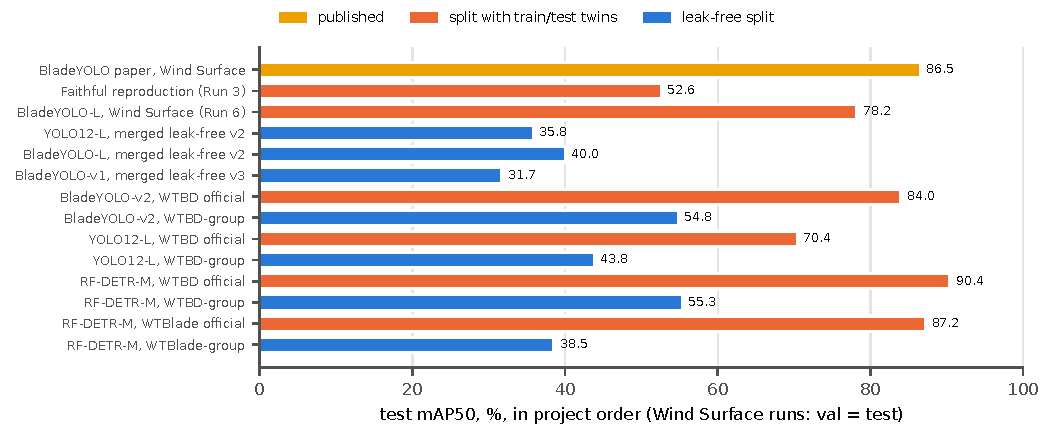
\includegraphics[width=\linewidth]{fig23_score_history}
\caption{Reported \mfifty at each stage of the project, in order. Every class-aware score above about 60 was measured on a split with train/test twins, including our own. Datasets differ between rows, so rows are not comparable as models; the point is the pattern.}
\label{fig:history}
\end{figure}

\begin{table}[!t]
\centering
\caption{Early runs on the original Wind Surface split (2{,}856/714), \mfifty/\mcoco on validation. Later analysis invalidated the conclusions drawn from them.}
\label{tab:runs}
\footnotesize
\begin{tabularx}{\linewidth}{@{}l X r r X@{}}
\toprule
Run & Architecture & \mfifty & \mcoco & Outcome \\
\midrule
1--2 & Faithful: DINOv3 + style injection + WTConv + Cross-Mamba & -- & -- & bf16, unfreezing, DDP failures; FFT NaNs \\
3 & Faithful, FFT detached, SGD, $\sim$283 ep & $\sim$52.6 & $\sim$28.0 & stagnated; closest reproduction \\
4 & BladeYOLO-S (8\,M), 400 ep & 64.3 & 37.3 & apparent ceiling \\
6 & BladeYOLO-L (57.2\,M), AdamW, 400 ep & 78.2 & 46.9 & ``breakthrough'' (leaked) \\
7 & Run 6 + ``Mamba'' + WIoU v3 & 77.0 & 47.8 & WIoU never ran; no scan \\
\bottomrule
\end{tabularx}
\end{table}

\subsection{Our Numbers Against Published Ones}
Table~\ref{tab:cross} brings every model we trained or reproduced together with the published results, across the three official and the two leak-free benchmarks. Read by column, it shows three things. No single model leads everywhere. The official columns are 25--50 points higher than the leak-free ones for the same model. And the published BladeYOLO numbers stand alone on the two protocols on which they were reported.

\begin{table*}[!t]
\centering
\caption{Comparison across all five benchmarks: \mfifty / \mcoco on the test set of each protocol (Wind Surface: its validation set, which serves as test). Official protocols are leaky (Table~\ref{tab:audit}); leak-free ones are scene-grouped (Section~\ref{sec:benchmarks}). Two-seed means where two seeds exist. Our values use the COCO-style evaluator. \hlnote{} Shaded: proposed method.}
\label{tab:cross}
\footnotesize
\setlength{\tabcolsep}{3.4pt}
\begin{tabular}{@{}l c cc cc cc cc cc@{}}
\toprule
& & \multicolumn{6}{c}{\textit{Official protocols (leaky)}} & \multicolumn{4}{c}{\textit{Leak-free protocols (ours)}} \\
\cmidrule(lr){3-8}\cmidrule(l){9-12}
& & \multicolumn{2}{c}{WTBD-official} & \multicolumn{2}{c}{Wind Surface} & \multicolumn{2}{c}{WTBlade-Defect} & \multicolumn{2}{c}{WTBD-group} & \multicolumn{2}{c}{WTBlade-group} \\
\cmidrule(lr){3-4}\cmidrule(lr){5-6}\cmidrule(lr){7-8}\cmidrule(lr){9-10}\cmidrule(l){11-12}
Model & Source & 50 & 50:95 & 50 & 50:95 & 50 & 50:95 & 50 & 50:95 & 50 & 50:95 \\
\midrule
\multicolumn{12}{@{}l}{\textit{Published}} \\
BladeYOLO~\cite{bladeyolo} & paper & -- & -- & \best{86.5} & \best{57.4} & \second{85.8}$^\ddagger$ & \best{74.6}$^\ddagger$ & -- & -- & -- & -- \\
YOLOv12-L, as reported in~\cite{bladeyolo} & paper & -- & -- & -- & -- & 83.3$^\ddagger$ & \second{71.9}$^\ddagger$ & -- & -- & -- & -- \\
\midrule
\multicolumn{12}{@{}l}{\textit{Our reproductions of BladeYOLO (before the code audit and the leak finding)}} \\
Faithful reimplementation (Run 3) & ours & -- & -- & 52.6 & 28.0 & -- & -- & -- & -- & -- & -- \\
BladeYOLO-L (Run 6) & ours & -- & -- & 78.2 & 46.9 & -- & -- & -- & -- & -- & -- \\
\midrule
\multicolumn{12}{@{}l}{\textit{YOLO family}} \\
YOLO12-L~\cite{yolov12} & ours & 69.0 & 37.7 & -- & -- & -- & -- & 40.0 & 18.5 & 32.2 & 13.3 \\
BladeYOLO-v2 without DINOv3 & ours & -- & -- & -- & -- & -- & -- & 31.8 & 15.2 & -- & -- \\
BladeYOLO-v2 (frozen DINOv3)$^\S$ & ours & 81.5 & 48.1 & -- & -- & -- & -- & \second{56.1} & 24.4 & \best{41.8} & \best{18.0} \\
\midrule
\multicolumn{12}{@{}l}{\textit{Detection transformers}} \\
RF-DETR-L~\cite{rfdetr} (G26) & ours & 88.9 & 59.5 & -- & -- & -- & -- & -- & -- & -- & -- \\
RF-DETR-M~\cite{rfdetr} (G26 / A0) & ours & \second{90.4} & \best{61.2} & 81.0 & \second{53.3} & \best{87.2} & 55.1 & 54.3 & \second{32.2} & 40.0 & 16.6 \\
RF-DETR-M + copy-paste (G27 A1) & ours & -- & -- & -- & -- & -- & -- & 55.0 & 31.7 & 40.6 & 16.9 \\
\ours RF-DETR-FP (G29) & ours & \best{90.9} & \second{59.9} & \second{82.1} & 51.7 & -- & -- & \best{58.9} & \best{34.4} & \second{41.0} & \second{17.3} \\
\bottomrule
\end{tabular}
\tabnote{$^\ddagger$On BladeYOLO's own unpublished 9:1 re-split of 5{,}326 WTBlade-Defect images, not the official 553-image test set. Wind Surface: the BladeYOLO paper reports 3{,}790 images, our public copy has 3{,}570. $^\S$ViT-S/16 on WTBD, ViT-B/16 on WTBlade-group. Run 3 and Run 6 were measured with weakened DINOv3 features and other code defects (Section~\ref{sec:history}). RF-DETR-FP on WTBlade-Defect official was not run (pre-registered: it does not fit a 12\,h T4 session).}
\end{table*}

Table~\ref{tab:official} and Fig.~\ref{fig:official-bladeyolo} give our scores on the official protocols beside the published ones. A generic detector with a standard recipe and no blade-specific modules reaches the level of the specialised models on two protocols, but not on Wind Surface.

\begin{table}[!t]
\centering
\caption{Official protocols in detail: this work against published results. \mfifty/\mcoco [95\% CI], single seed, selected on validation; intervals are image-level. BladeYOLO's WTBlade numbers use its own unpublished 9:1 re-split, so that row is not directly comparable. $^\dagger$Ultralytics \texttt{val}; other rows of ours use the COCO-style evaluator. \hlnote{} (within each protocol)}
\label{tab:official}
\footnotesize
\setlength{\tabcolsep}{3pt}
\begin{tabularx}{\linewidth}{@{}X l@{}}
\toprule
Model & \mfifty / \mcoco \\
\midrule
\multicolumn{2}{@{}l}{\textit{WTBD-official (test 161)}} \\
YOLO12-L (ours)$^\dagger$ & 70.4 / 38.8 \\
BladeYOLO-v2 (ours)$^\dagger$ & 84.0 / 49.3 \\
RF-DETR-M 768, constant LR (G25) & \second{90.5} \ci{86.3}{94.4} / \second{60.2} \ci{55.6}{65.3} \\
RF-DETR-M 768, cosine (G26) & 90.4 \ci{85.8}{94.7} / \best{61.2} \ci{56.5}{66.1} \\
RF-DETR-L 704, cosine (G26) & 88.9 / 59.5 \\
\ours RF-DETR-FP 768 (G29) & \best{90.9} \ci{87.0}{94.6} / 59.9 \ci{55.2}{65.5} \\
\midrule
\multicolumn{2}{@{}l}{\textit{Wind Surface (val 714)}} \\
BladeYOLO~\cite{bladeyolo} & \best{86.5} / \best{57.4} \\
Faithful reimplementation (Run 3) & 52.6 / 28.0 \\
Our best leaky BladeYOLO-L (Run 6) & 78.2 / 46.9 \\
RF-DETR-M 640, 60 ep, constant (G25) & 81.8 \ci{78.0}{85.4} / 51.4 \ci{48.3}{55.0} \\
RF-DETR-M 640, 100 ep, cosine (G26) & 81.0 \ci{77.1}{84.9} / \second{53.3} \ci{50.0}{57.0} \\
\ours RF-DETR-FP 640, 100 ep (G29) & \second{82.1} \ci{78.4}{86.0} / 51.7 \ci{48.5}{55.4} \\
\midrule
\multicolumn{2}{@{}l}{\textit{WTBlade-Defect (test 553)}} \\
BladeYOLO~\cite{bladeyolo} & 85.8 / \best{74.6} \\
YOLOv12-L, as reported there & 83.3 / \second{71.9} \\
RF-DETR-M 640, 25 ep, constant (G25) & \best{87.4} \ci{84.4}{90.9} / 52.5 \ci{49.6}{56.2} \\
RF-DETR-M 640, 40 ep, cosine (G26) & \second{87.2} \ci{84.0}{90.6} / 55.1 \ci{52.0}{59.1} \\
\bottomrule
\end{tabularx}
\end{table}

\begin{figure*}[!t]
\centering
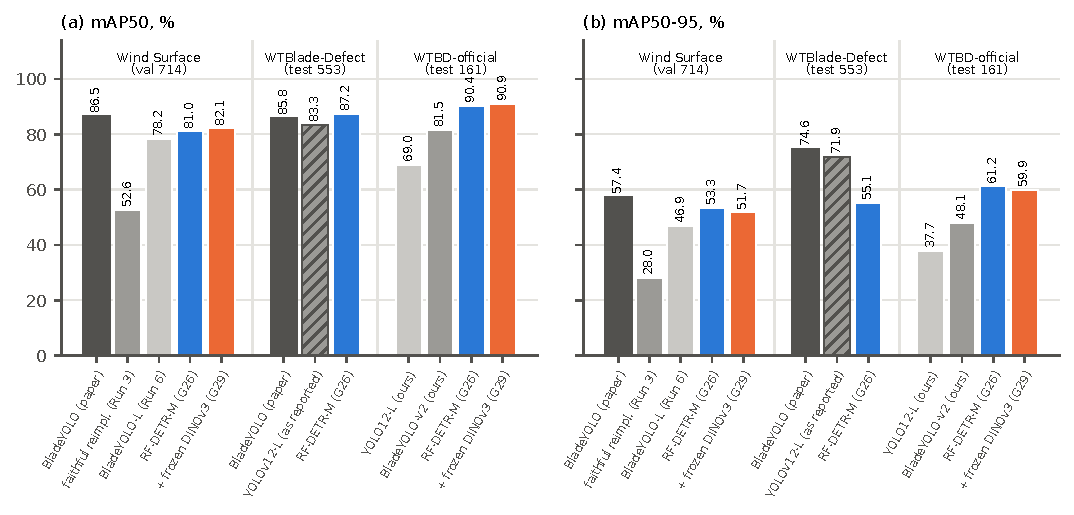
\includegraphics[width=0.92\textwidth]{fig32_official_vs_bladeyolo}
\caption{Official protocols: the BladeYOLO paper (dark), values reported in that paper for its baseline (hatched), our reproductions and BladeYOLO-style models (grey), RF-DETR-M with the G26 recipe (blue) and RF-DETR-FP (orange). Our values use the COCO-style evaluator. On WTBD-official the BladeYOLO paper reports no number. Every value in this figure was measured on a split in which most test images have a training twin (Table~\ref{tab:audit}).}
\label{fig:official-bladeyolo}
\end{figure*}

To our knowledge, the WTBD-official rows are the best reported on that protocol; the dataset paper itself gives no detection baselines~\cite{wtbd}. On WTBlade-Defect, RF-DETR-M exceeds BladeYOLO's \mfifty (87.2 against 85.8) on a different split of the same data, while BladeYOLO's \mcoco (74.6) is 19.5 points higher. On Wind Surface, our best is 4.4 \mfifty and 4.1 \mcoco below the paper. Our copy has 3{,}570 images against the 3{,}790 the paper reports, so the splits differ.

\textbf{The \mcoco/\mfifty ratio.} The ratio on WTBlade is 0.87 in the BladeYOLO paper and 0.86 for its YOLOv12-L baseline. RF-DETR's ratio is 0.71 on WTBlade copies of training frames, 0.63 on all official test images and 0.34 on no-twin images. Across all our leak-free runs it spans 0.41--0.60. A ratio of 0.87 sits above every one of these. This is consistent with near-duplicate copies falling on both sides of a random split, whose boxes a detector can reproduce to the pixel. It is not proof, because that split is not available.

\subsection{Leaked and No-Twin Test Images}
Using the per-image flags from the audit, we score the same official runs on the two subsets (Table~\ref{tab:subsets}, Fig.~\ref{fig:leak}).

\begin{table*}[!t]
\centering
\caption{The same official runs on leaked and no-twin test images (COCO-style evaluator, \mfifty/\mcoco [95\% CI], post hoc). Subset sizes (images/boxes): WTBD 125/185 leaked and 36/53 no twin; Wind Surface 600/1{,}169 and 114/158; WTBlade 499/1{,}235 and 43/91. \hlnote{} (within each protocol; one-run protocols are not ranked)}
\label{tab:subsets}
\footnotesize
\begin{tabularx}{\textwidth}{@{}X l l l@{}}
\toprule
Protocol, run & All & Leaked & No twin \\
\midrule
WTBD-official, YOLO12-L & 69.0 / 37.7 & 69.7 / 38.5 & 70.0 / 35.2 \\
WTBD-official, BladeYOLO-v2 & 81.5 / 48.1 & 82.6 / 48.9 & 81.5 / 47.8 \\
WTBD-official, RF-DETR-L 704 cosine (G26) & 88.9 / 59.5 & 90.3 / 61.1 & 77.4 \ci{63.6}{92.4} / \best{53.5} \ci{40.8}{65.6} \\
WTBD-official, RF-DETR-M 768 cosine (G26) & \second{90.4} / \best{61.2} & \second{91.5} / \best{63.9} & \second{81.6} \ci{69.1}{93.2} / 49.9 \ci{40.4}{61.1} \\
\ours WTBD-official, RF-DETR-FP (G29) & \best{90.9} / \second{59.9} & \best{91.9} / \second{62.0} & \best{90.8} \ci{79.5}{95.3} / \second{52.5} \ci{43.2}{63.5} \\
\midrule
Wind Surface, RF-DETR-M cosine (G26) & 81.0 / \best{53.3} & 83.3 / \best{55.1} & 59.2 \ci{49.0}{68.1} / \best{37.6} \ci{29.9}{45.4} \\
\ours Wind Surface, RF-DETR-FP (G29) & \best{82.1} / 51.7 & \best{84.9} / 53.8 & \best{61.0} \ci{53.5}{72.0} / 35.3 \ci{30.4}{45.3} \\
\midrule
WTBlade-Defect, RF-DETR-M cosine (G26) & 87.2 / 55.1 & 90.8 / 59.4 & \textbf{50.4} \ci{38.5}{64.0} / \textbf{17.2} \ci{13.5}{23.4} \\
\quad copies of a training frame (360) & & \textbf{98.2} \ci{97.7}{98.8} / \textbf{69.8} \ci{67.8}{72.5} & \\
\quad same scene, not a copy (139) & & 65.7 / 30.1 & \\
\bottomrule
\end{tabularx}
\end{table*}

\begin{figure}[!t]
\centering
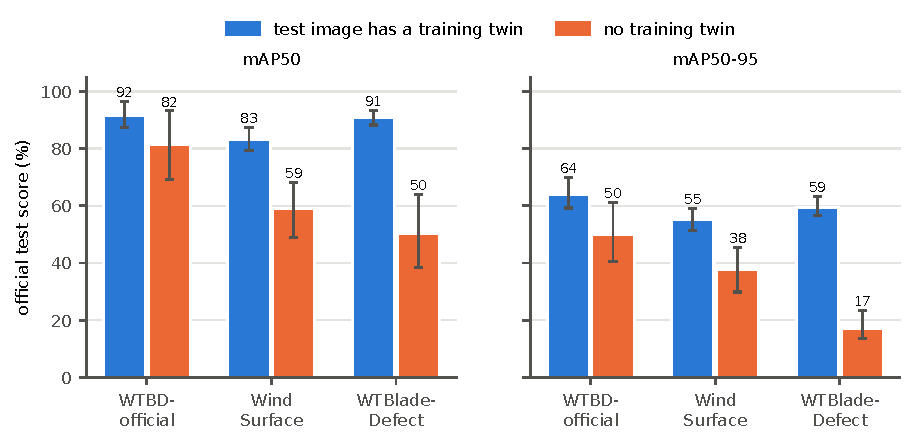
\includegraphics[width=\linewidth]{fig1_leak_subsets}
\caption{Official-protocol scores of the best RF-DETR-M run on leaked and no-twin test images, with image-bootstrap 95\% intervals.}
\label{fig:leak}
\end{figure}

WTBlade-Defect's official number is mostly its copies: 98.2 on copies of training frames and 50.4 with no same-scene training image. The independently built WTBlade-group benchmark agrees from a different direction. Its RF-DETR-M runs score 16.2--17.3 \mcoco (Table~\ref{tab:leakfree}) against 17.2 here, and their 38.5--41.6 \mfifty lies inside this small subset's interval of \ci{38.5}{64.0}. WTBD's no-twin subset is too small to read on its own: it holds a single box each of craze, thunderstrike and crack, and corrosion is the only class with a clear drop (\apfifty 97 to 54). The split comparison below is therefore the stronger evidence for WTBD.

\subsection{Same Detector, Only the Split Differs}
Table~\ref{tab:split-only} and Fig.~\ref{fig:inflation} compare models trained on the same 1{,}065 WTBD images, with the official split against the scene-grouped one.

\begin{table}[!t]
\centering
\caption{Same recipe, only the WTBD split differs: test \apfifty by class and overall \mfifty/\mcoco (O = official, G = group). BladeYOLO-v2 (BYv2) and YOLO12-L use Ultralytics \texttt{val}; RF-DETR-M uses the COCO-style evaluator, seed 0, 768\,px, 100 epochs on both splits. \best{Red bold}: best of the three models within each split.}
\label{tab:split-only}
\footnotesize
\setlength{\tabcolsep}{2.6pt}
\begin{tabular}{@{}l rr rr rr@{}}
\toprule
& \multicolumn{2}{c}{BYv2} & \multicolumn{2}{c}{YOLO12-L} & \multicolumn{2}{c}{RF-DETR-M} \\
\cmidrule(lr){2-3}\cmidrule(lr){4-5}\cmidrule(l){6-7}
Class & O & G & O & G & O & G \\
\midrule
crack & \best{99.1} & 38.1 & 85.4 & 38.4 & 95.3 & \best{61} \\
craze & 90.9 & 7.6 & 62.2 & 6.5 & \best{95.3} & \best{9} \\
hide\_craze & 80.0 & 56.9 & 63.9 & 52.6 & \best{80.3} & \best{71} \\
surface\_injure & 81.6 & 74.7 & 71.1 & 62.9 & \best{91.0} & \best{83} \\
thunderstrike & \best{99.5} & \best{98.0} & 93.8 & 41.8 & 94.3 & 64 \\
corrosion & 52.7 & 53.8 & 46.0 & \best{60.8} & \best{86.0} & 46 \\
\midrule
\mfifty & 84.0 & 54.8 & 70.4 & 43.8 & \best{90.4} & \best{55.3} \\
\mcoco & 49.3 & 24.5 & 38.8 & 20.6 & \best{61.2} & \best{33.2} \\
\bottomrule
\end{tabular}
\end{table}

\begin{figure}[!t]
\centering
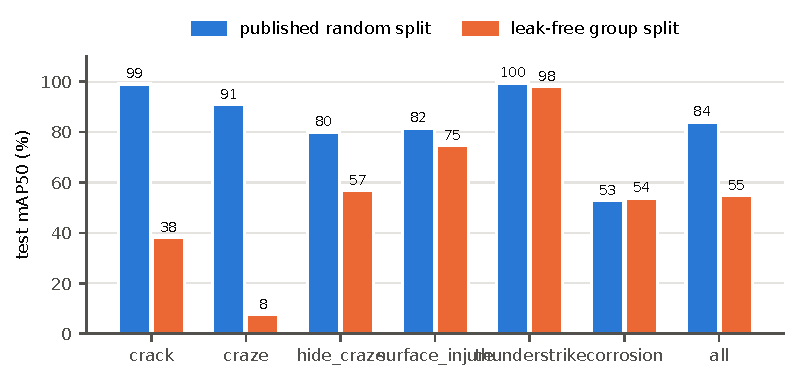
\includegraphics[width=0.95\linewidth]{fig3_wtbd_inflation}
\caption{Inflation per class on WTBD for BladeYOLO-v2 and YOLO12-L, with the same recipe on the official and the group split.}
\label{fig:inflation}
\end{figure}

The inflation does not depend on the model: $+29.2$ \mfifty for BladeYOLO-v2, $+26.6$ for YOLO12-L and $+35.1$ for RF-DETR-M, with \mcoco multiplied by 2.0, 1.9 and 1.8. On WTBlade the pair is 87.2/55.1 officially against 38.5/16.2 on WTBlade-group. That is not a pure split comparison, because WTBlade-group also keeps one frame per source and trains for 60 rather than 40 epochs.

\subsection{Tuning on the Official Splits Rewards Memorisation}
Between G25 and G26 we made one tuning step in the usual spirit. We moved to a cosine schedule (and, on two protocols, longer training) because the official numbers improved. Table~\ref{tab:tuning} decomposes what that step bought (post hoc).

\begin{table*}[!t]
\centering
\caption{What one tuning step bought, and what RF-DETR-FP changed. Paired image bootstrap, $\Delta$\mcoco in points on the same images. Interaction $=\Delta_{\mathrm{leaked}}-\Delta_{\mathrm{no\,twin}}$, with the subsets resampled independently.}
\label{tab:tuning}
\footnotesize
\begin{tabularx}{\textwidth}{@{}X l l l l@{}}
\toprule
Protocol (change) & $\Delta$ all & $\Delta$ leaked & $\Delta$ no twin & Interaction, $P(>0)$ \\
\midrule
\multicolumn{5}{@{}l}{\textit{G26 tuning step (post hoc)}} \\
WTBD-official (constant $\rightarrow$ cosine) & $+1.0$ \ci{-1.2}{+3.0} & $+1.8$ \ci{-0.1}{+4.0} & $-8.1$ \ci{-13.4}{+0.2} & $+9.9$ \ci{+1.1}{+15.8}, 0.993 \\
Wind Surface (60 ep constant $\rightarrow$ 100 ep cosine) & $+1.8$ \ci{+0.5}{+3.1} & $+2.3$ \ci{+0.9}{+3.8} & $-1.5$ \ci{-4.2}{+1.4} & $+3.8$ \ci{+0.7}{+7.0}, 0.988 \\
WTBlade-Defect (25 ep constant $\rightarrow$ 40 ep cosine) & $+2.6$ \ci{+1.1}{+3.9} & $+3.5$ \ci{+2.0}{+5.0}; copies $+5.4$ & $-4.0$ \ci{-7.2}{+0.1} & $+7.4$ \ci{+3.0}{+11.1}, 1.000 \\
\midrule
\multicolumn{5}{@{}l}{\textit{RF-DETR-FP $-$ its G26 twin (pre-registered benchmark entries)}} \\
\ours WTBD-official & $-1.2$ \ci{-3.3}{+1.0} & $-1.9$ \ci{-3.9}{+0.6} & $+2.6$ \ci{-2.1}{+7.2} & $-4.5$ \ci{-9.0}{+0.9}, 0.048 \\
\ours Wind Surface & $-1.5$ \ci{-2.9}{-0.3} & $-1.3$ \ci{-2.6}{+0.1} & $-2.3$ \ci{-6.7}{+2.0} & $+1.0$ \ci{-3.7}{+5.4}, 0.593 \\
\bottomrule
\end{tabularx}
\end{table*}

\begin{figure}[!t]
\centering
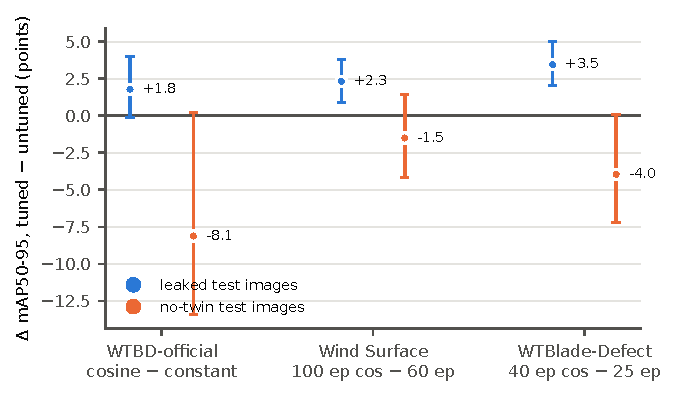
\includegraphics[width=\linewidth]{fig2_tuning_memorisation}
\caption{The G26 tuning step of Table~\ref{tab:tuning}: the gains sit on leaked images, and the same change lowers the no-twin score.}
\label{fig:tuning}
\end{figure}

On every protocol the gain of the tuning step sits on leaked images, and the same change lowers the score on images without a twin (Fig.~\ref{fig:tuning}). At \mfifty the change is $-0.2$ to $-0.8$ overall and $-5.0$ to $-6.0$ on no-twin images. The interaction excludes zero on all three protocols. This applies to our own G26 numbers, which stay in Table~\ref{tab:official} labelled as what they are. Two confounds remain: on Wind Surface and WTBlade-Defect the epoch count also changed (on WTBD only the schedule changed, with the same pattern), and this is one tuning step, not a study of tuning in general.

RF-DETR-FP moves in the opposite direction. On WTBD-official its change sits on the no-twin images ($+2.6$ \mcoco, $+9.2$ \mfifty), and the interaction is negative. By the rule fixed at pre-registration (no-twin $\Delta\geq0$), its official change is not memorisation. It is not an official \mcoco gain either, which falls on both protocols and significantly so on Wind Surface. A leaderboard reading would discard RF-DETR-FP; the leak-aware reading shows it is the only change we made whose official effect points towards unseen scenes.

A second reading comes from the leaderboard itself. RF-DETR-M leads BladeYOLO-v2 on WTBD-official by $+13.2$ \ci{+8.2}{+17.4} \mcoco on all images, but by only $+2.1$ \ci{-5.3}{+19.8} on the 36 no-twin images. That official lead is therefore not established on unseen images. RF-DETR-FP leads BladeYOLO-v2 by $+11.9$ \ci{+7.4}{+16.2} on all images and by $+4.7$ \ci{-4.2}{+23.4} on no-twin images.

\subsection{Consequence for Deployment: Leaked Calibration Breaks Recall Guarantees}
An inspection system should promise a bound on missed defects. Conformal risk control~\cite{crc} chooses a confidence threshold $\hat\lambda$ so that the expected share of missed defects is at most $\alpha$:
\begin{equation}
\hat\lambda=\sup\Big\{\lambda:\ \tfrac{n}{n+1}\hat{L}_n(\lambda)+\tfrac{1}{n+1}\leq\alpha\Big\},
\label{eq:crc}
\end{equation}
where $\hat{L}_n(\lambda)$ is the empirical miss rate on $n$ calibration units at threshold $\lambda$. A defect counts as flagged if at least 50\% of its box is covered by predictions above the threshold. We calibrate on seen or unseen scenes and always deploy on unseen scenes (Table~\ref{tab:conformal}, Fig.~\ref{fig:conformal}).

\begin{table}[!t]
\centering
\caption{Conformal recall guarantee, target $\leq$10\% missed (BladeYOLO-v2; 500 draws of 100 calibration images, or of scene groups as units).}
\label{tab:conformal}
\footnotesize
\begin{tabularx}{\linewidth}{@{}X X r r@{}}
\toprule
Calibrated on & Deployed on & Miss rate & Violating \\
\midrule
Seen scenes (group train), images & unseen scenes & \textbf{31.5\%} & 100\% \\
Seen scenes, scene units & unseen scenes & 28.8\% & 100\% \\
Unseen scenes (group val), images & unseen scenes & 6.3\% & 0\% \\
Unseen scenes, scene units & unseen scenes & 4.7\% & 1\% \\
Official val (leaky) & official test, with twin & 12.6\% & 91\% \\
Official val (leaky) & official test, no twin & \textbf{25.9\%} & 100\% \\
\bottomrule
\end{tabularx}
\end{table}

\begin{figure}[!t]
\centering
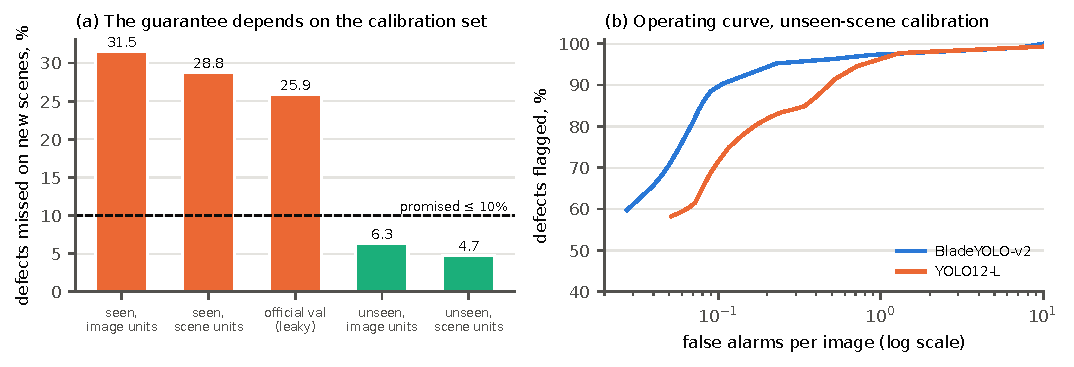
\includegraphics[width=\linewidth]{fig14_conformal}
\caption{(a) Realised miss rate on new scenes, by calibration set. (b) Operating curve with scene units, calibrated on unseen scenes. At 0.1 false alarms per image BladeYOLO-v2 flags about 90\% of defects on new scenes, YOLO12-L about 71\%. One test set of 58 scenes; the curve has no interval.}
\label{fig:conformal}
\end{figure}

Models are overconfident on what they memorised, so a threshold calibrated on seen scenes is too high for new data. Calibration data must therefore be split by scene, as test data must. The honest calibration is cheap: 0.2 instead of 0.1 false alarms per image. With only 60 calibration and 58 deployment scenes from one site, the validation and test groups are not perfectly exchangeable. YOLO12-L still misses 12.3\% with scene-unit calibration on unseen scenes, violating the bound in 71\% of draws.

\section{Leak-Free Results: What Helps}
\label{sec:leakfree}

\subsection{The Benchmark at Full Labels}
Table~\ref{tab:leakfree}, Fig.~\ref{fig:benchmark} and Fig.~\ref{fig:perclass} give the benchmark, all scored with one evaluator on cached predictions.

\begin{table}[!t]
\centering
\caption{Leak-free benchmark, full labels: test \mfifty/\mcoco, COCO-style evaluator; mean of two seeds where marked (2), per-seed values in Table~\ref{tab:newruns}. The A0 seeds are the two T4 runs paired with RF-DETR-FP; an A100 rerun of A0 seed 1 scored 54.8/32.2 and 41.0/16.9. Cross-architecture rows have no paired interval, so treat them as point estimates. \hlnote{} Shaded: proposed method.}
\label{tab:leakfree}
\footnotesize
\setlength{\tabcolsep}{3pt}
\begin{tabularx}{\linewidth}{@{}X cc cc@{}}
\toprule
& \multicolumn{2}{c}{WTBD-group} & \multicolumn{2}{c}{WTBlade-group} \\
& \multicolumn{2}{c}{\scriptsize 161 img, 58 scenes} & \multicolumn{2}{c}{\scriptsize 332 frames, 177 scenes} \\
\cmidrule(lr){2-3}\cmidrule(l){4-5}
Model & 50 & 50:95 & 50 & 50:95 \\
\midrule
YOLO12-L & 40.0 & 18.5 & 32.2 & 13.3 \\
BladeYOLO-v2 without DINOv3 & 31.8 & 15.2 & -- & -- \\
BladeYOLO-v2 (ViT-S / ViT-B) & \second{56.1} & 24.4 & \best{41.8} & \best{18.0} \\
RF-DETR-M, A0 (2) & 54.3 & 32.2 & 40.0 & 16.6 \\
\quad + copy-paste, A1 (2) & 55.0 & 31.7 & 40.6 & 16.9 \\
\quad + copy-paste + in-domain SSL, A2 & 49.6 & 27.4 & 40.1 & 16.1 \\
\quad + copy-paste + multi-dataset, A3 & 55.3 & \second{33.2} & \second{41.7} & 16.6 \\
\ours RF-DETR-FP (ours) (2) & \best{58.9} & \best{34.4} & 41.0 & \second{17.3} \\
\bottomrule
\end{tabularx}
\end{table}

\begin{figure*}[!t]
\centering
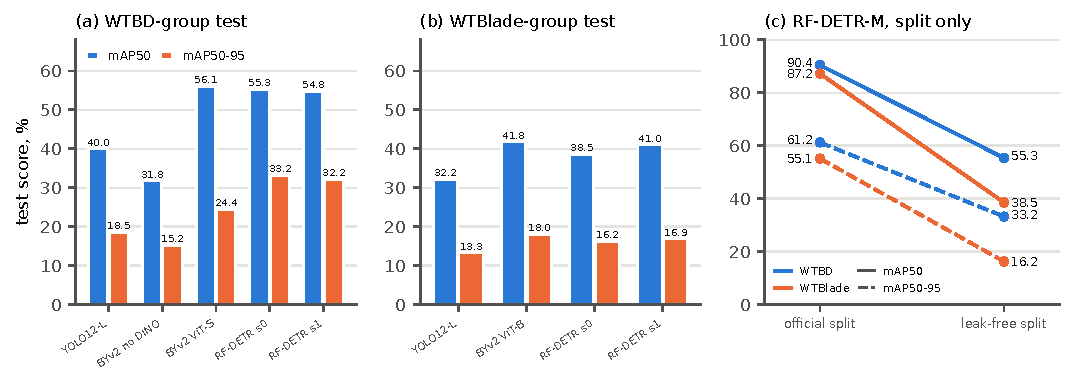
\includegraphics[width=\textwidth]{fig17_benchmark}
\caption{(a, b) Leak-free test scores by model (BYv2: BladeYOLO-v2; s0, s1: seeds). (c) RF-DETR-M on the official and leak-free splits of the same data.}
\label{fig:benchmark}
\end{figure*}

\begin{figure*}[!t]
\centering
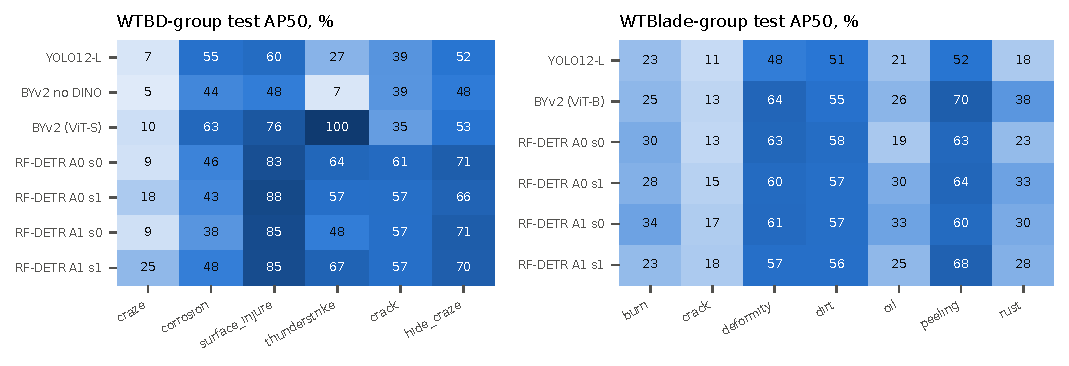
\includegraphics[width=0.96\textwidth]{fig24_per_class}
\caption{Per-class test \apfifty on the leak-free benchmarks. Note the seed-to-seed swings within RF-DETR on rare classes (craze 9--25, thunderstrike 48--67), and BladeYOLO-v2's thunderstrike 100, which rests on 3 test scenes.}
\label{fig:perclass}
\end{figure*}

Four points stand out:
\begin{itemize}
\item \textbf{The ranking depends on the dataset.} RF-DETR-M leads on WTBD-group by 7--9 \mcoco points over BladeYOLO-v2. On WTBlade-group, however, the frozen ViT-B BladeYOLO-v2 (18.0) is ahead of every RF-DETR run, RF-DETR-FP included (16.1--17.3). A ``generic detector is strongest'' claim holds on one benchmark.
\item \textbf{On WTBD the RF-DETR gain is box quality, not finding.} RF-DETR-M's \mfifty is level with BladeYOLO-v2 (55.3 and 53.2 against 56.1), while its \mcoco is 7--9 points higher. This matches the extent analysis of Section~\ref{sec:anatomy}.
\item \textbf{Classification costs RF-DETR points.} Scoring A0 with classes merged gives 66.1/40.5 on WTBD-group and 50.1/21.3 on WTBlade-group (Table~\ref{tab:g28}), about 11 \apfifty points above its class-aware score. BladeYOLO-v2's class-agnostic and class-aware \apfifty are about equal (56.3 against 56.1), while YOLO12-L shows a gap like RF-DETR's (48.5 against 40.0).
\item \textbf{The earlier BladeYOLO-v2 win over YOLO12-L rests largely on thunderstrike.} The scene bootstrap gives $+16.1$ \ci{+2.5}{+28.4} \mfifty and $+5.9$ \ci{+0.5}{+16.9} \mcoco. Without the two classes seen in at most 3 test scenes, however, the \mfifty gain is $+5.2$ \ci{-2.7}{+13.5}.
\end{itemize}

\subsection{RF-DETR-FP: Pre-Registered Test}
\label{sec:fp-results}
\textbf{Protocol} (G29, fixed before any run). Each RF-DETR-FP run is paired with an existing run of identical recipe on the same hardware type (Kaggle T4, fp16). The primary claim P compares FP and A0 on leak-free test \mcoco with the paired scene bootstrap of~\eqref{eq:bootstrap}, averaged over seeds 0 and 1 (2{,}000 replicates). It passes if the point estimate is $>0$ on each dataset and the dataset mean has $P(>0)\geq0.95$; this is the bar G27 failed. Reported with it, and not gating, are the validation split in the same form, WTBD-group without its six pixel-twin test images, per-class AP, the error anatomy and a comparison with every other architecture. Two mechanism predictions were also written down: that the gain is larger on WTBlade-group than on WTBD-group, and that on WTBD it sits in the rare, confusable classes. A secondary claim S asks the same question at 25\% labels (FP against V1 over four subsets). The official protocols are benchmark entries, not tests (Section~\ref{sec:official}).

\begin{table}[!t]
\centering
\caption{G29 primary claim (P): RF-DETR-FP $-$ RF-DETR-M (A0), leak-free \mcoco, paired scene bootstrap, mean of seeds 0 and 1.}
\label{tab:g29}
\footnotesize
\setlength{\tabcolsep}{2.2pt}
\begin{tabular}{@{}l l l l l@{}}
\toprule
& A0 s0 / s1 & FP s0 / s1 & FP $-$ A0 [95\% CI] & $P(>0)$ \\
\midrule
WTBD-group test & 33.2 / 31.2 & 34.3 / 34.5 & $+2.18$ \ci{-0.8}{+4.4} & 0.916 \\
WTBlade-group test & 16.2 / 16.9 & 17.3 / 17.2 & $+0.72$ \ci{-0.6}{+1.9} & 0.866 \\
\textbf{mean, test} & & & $\mathbf{+1.45}$ \ci{-0.2}{+2.7} & \textbf{0.958} \\
\midrule
WTBD-group val & 40.1 / 40.2 & 42.2 / 39.0 & $+0.43$ \ci{-3.1}{+3.3} & 0.569 \\
WTBlade-group val & 15.7 / 16.6 & 16.1 / 16.1 & $-0.02$ \ci{-2.8}{+2.2} & 0.465 \\
mean, val & & & $+0.20$ \ci{-2.0}{+1.9} & 0.526 \\
\bottomrule
\end{tabular}
\end{table}

\begin{figure*}[!t]
\centering
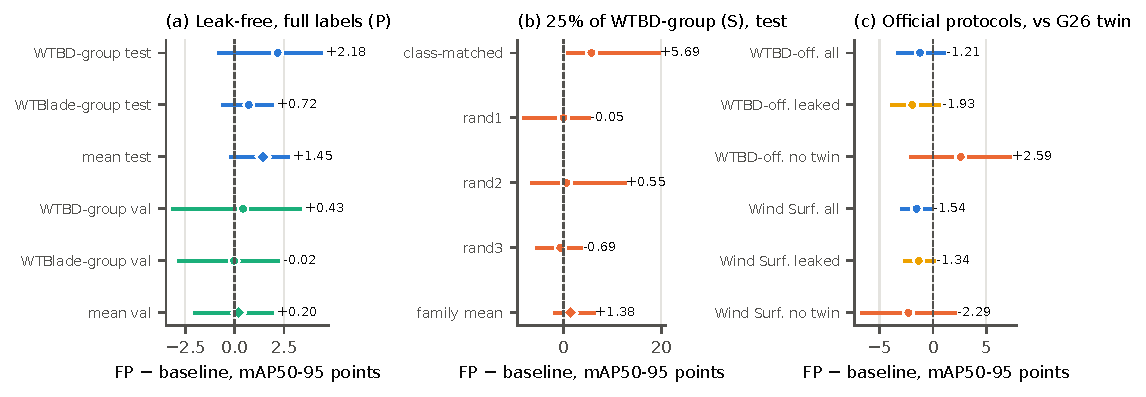
\includegraphics[width=\textwidth]{fig29_g29_effects}
\caption{RF-DETR-FP paired effects in \mcoco points with 95\% intervals. (a) Primary claim on the leak-free benchmarks, test (blue) and validation (green); diamonds mark dataset means. (b) Secondary claim at 25\% of WTBD-group scenes, four subsets, test. (c) Official protocols against the G26 twin, on all, leaked and no-twin test images (image bootstrap).}
\label{fig:g29-effects}
\end{figure*}

\textbf{Result.} By the pre-registered rule the primary claim \emph{passes} (Table~\ref{tab:g29}, Fig.~\ref{fig:g29-effects}a). The effect is positive on both datasets, and the mean has $P(>0)=0.958$ against a bar of 0.95. On test, both FP seeds are above both A0 seeds on both datasets. RF-DETR-FP reaches 34.4 \mcoco on WTBD-group (mean of seeds), the best result on that benchmark by any model, and 17.3 on WTBlade-group. \mfifty rises more than \mcoco: 54.3 to 58.9 on WTBD-group and 40.0 to 41.0 on WTBlade-group. Without WTBD-group's six pixel-twin test images the gain is $+1.97$ (31.7 to 33.6), so those images do not carry it.

\textbf{Honest strength: narrow.} Validation does not confirm the gain ($+0.20$, $P=0.53$). The rule is decided on test, as for G27, so this does not change the verdict. It is, however, the pattern of an earlier hypothesis (H5) that passed narrowly on test with a flat validation result and then failed to replicate. The WTBD effect ($+2.2$) is about the size of A0's own seed spread there (33.2 against 31.2). And both mechanism predictions fail. The gain is larger on WTBD-group than on WTBlade-group ($+2.18$ against $+0.72$), the reverse of the prediction. On WTBD it sits in surface\_injure ($+5.8$) and craze ($+3.8$) rather than in thunderstrike ($+1.1$) and crack ($+1.4$) (Fig.~\ref{fig:g29-perclass}). The error anatomy barely moves: hits rise from 71.1 to 71.9\% and ``ranked low'' falls from 25.1 to 24.3\% on WTBD, and ``no box'' falls from 7.2 to 6.5\% on WTBlade. The effect looks real on test, but it is not where the evidence that motivated it said it would be.

\textbf{Against other architectures.} On WTBD-group, RF-DETR-FP (34.4) is above every other architecture: BladeYOLO-v2 24.4, YOLO12-L 18.5 and RF-DETR-M 31.2--33.2. On WTBlade-group (17.3) it is still below the frozen-DINOv3 BladeYOLO-v2 ViT-B (18.0, single run), though above YOLO12-L (13.3). The pre-registered ``beats every architecture on both leak-free tests'' condition is therefore \emph{not} met.

\begin{table}[!t]
\centering
\caption{G29 secondary claim (S): 25\% of WTBD-group scenes, RF-DETR-FP $-$ RF-DETR-M (V1), seed 0, 576\,px, \mcoco, scene bootstrap.}
\label{tab:g29s}
\footnotesize
\setlength{\tabcolsep}{3pt}
\begin{tabular}{@{}l l l l l@{}}
\toprule
Subset & V1 & FP & FP $-$ V1 [95\% CI] & $P(>0)$ \\
\midrule
class-matched & 18.9 & 24.6 & $+5.69$ \ci{+0.8}{+19.5} & 0.981 \\
random 1 & 20.5 & 20.4 & $-0.05$ \ci{-8.1}{+5.2} & 0.420 \\
random 2 & 21.5 & 22.1 & $+0.55$ \ci{-6.5}{+12.5} & 0.592 \\
random 3 & 14.7 & 14.1 & $-0.69$ \ci{-5.5}{+3.6} & 0.413 \\
family mean, test & & & $+1.38$ \ci{-1.8}{+6.2} & 0.856 \\
family mean, val & & & $+1.41$ \ci{-0.3}{+4.2} & 0.953 \\
\bottomrule
\end{tabular}
\end{table}

\textbf{Low labels.} The secondary claim fails (Table~\ref{tab:g29s}). The family mean is $+1.38$, $P=0.856$, positive on 2 of 4 subsets, although validation is positive on all four. At 25\% labels, RF-DETR-FP is therefore not the low-label lever that frozen DINOv3 was for the YOLO family. Subset luck still dominates: the class-matched subset alone moves by $+5.7$.

\begin{figure}[!t]
\centering
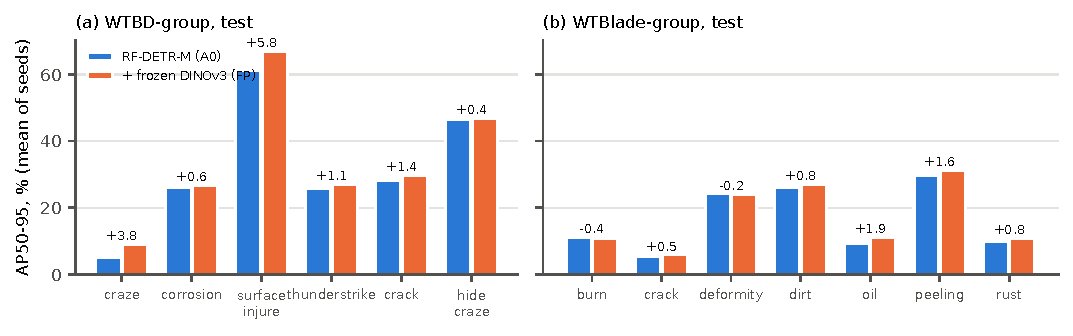
\includegraphics[width=\linewidth]{fig31_g29_perclass}
\caption{Per-class test AP$_{50:95}$ of RF-DETR-M (A0) and RF-DETR-FP, mean of two seeds; the label above each pair is the change. The gain sits in frequent classes (surface\_injure, craze; oil, peeling), not in the rare ones the motivating evidence pointed to.}
\label{fig:g29-perclass}
\end{figure}

\begin{figure*}[!t]
\centering
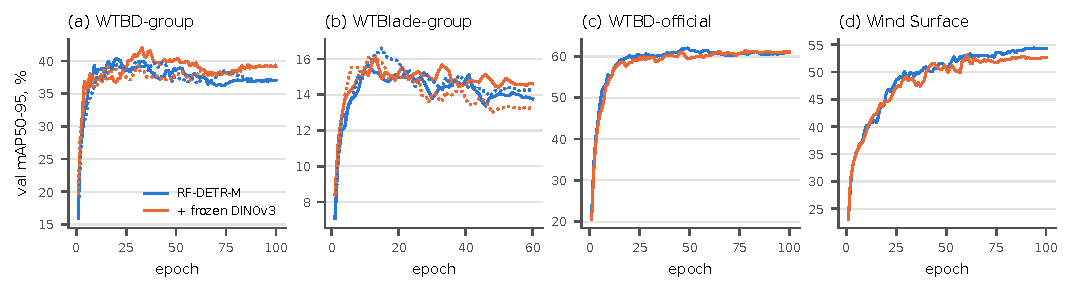
\includegraphics[width=\textwidth]{fig30_g29_curves}
\caption{Validation \mcoco (EMA) per epoch, RF-DETR-M against RF-DETR-FP with identical recipes. Solid: seed 0; dotted: seed 1. (a, b) Leak-free benchmarks. (c, d) Official protocols. On the leak-free splits both models peak early and drift, so EMA checkpoint selection matters. FP's curve stays higher late in training on WTBD-group, but its selected checkpoint does not separate on validation.}
\label{fig:g29-curves}
\end{figure*}

\begin{figure*}[!t]
\centering
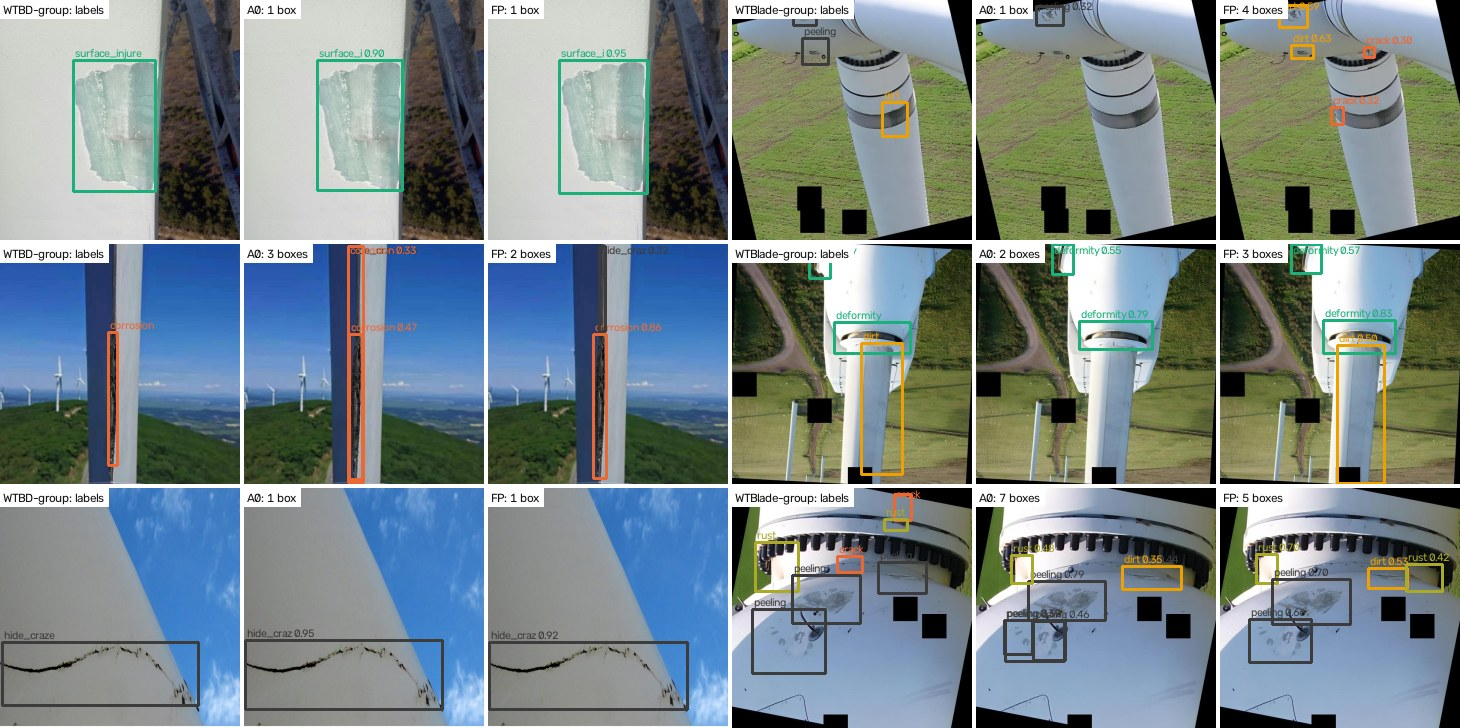
\includegraphics[width=\textwidth]{fig33_g29_predictions}
\caption{Labels, RF-DETR-M (A0) and RF-DETR-FP (seed 0) on random test images of WTBD-group (left three columns) and WTBlade-group (right three), fixed seed, boxes with confidence $\geq0.3$. Black squares in WTBlade-group are the Roboflow export's offline cutout, which the frames retain.}
\label{fig:g29-pred}
\end{figure*}

Fig.~\ref{fig:g29-curves} shows the training curves, and Fig.~\ref{fig:g29-pred} shows predictions on random test images. On the official protocols (Table~\ref{tab:tuning}, Fig.~\ref{fig:g29-effects}c), RF-DETR-FP raises \mfifty and lowers \mcoco. Its WTBD change sits on the no-twin images, and on Wind Surface it does not close the gap to BladeYOLO ($-4.4$ \mfifty, $-5.7$ \mcoco). By class on Wind Surface, thunderstrike improves (\apfifty 69 to 76) and surface\_eye falls (93 to 88).

\textbf{Verdict.} RF-DETR-FP passes its pre-registered primary test, by a narrow margin that validation does not support. It is the strongest leak-free RF-DETR result in this study, and the best WTBD-group result of any model. The honest wording is: a small gain ($+1.5$ points mean) that passes on test and is not confirmed on validation. It is not a low-label method, its gain is not where the motivating evidence predicted, and on the leaky official protocols it does not beat BladeYOLO's Wind Surface numbers. As pre-registered, we ran no rescue runs.

\subsection{Where the YOLO-Family Advantage Comes From: DINOv3 Ablation}
\label{sec:ablation}
We removed only the frozen DINOv3 features from BladeYOLO-v2, keeping deformable refinement, selective scan and WIoU. We then trained at 25\%, 50\% and 100\% of the labelled scenes (Table~\ref{tab:ablation}, Fig.~\ref{fig:curve}).

\begin{table*}[!t]
\centering
\caption{DINOv3 ablation and learning curve on WTBD-group: test \mcoco by labelled fraction, scene bootstrap for differences. \hlnote{} (among the three models)}
\label{tab:ablation}
\footnotesize
\begin{tabular}{@{}l l l l@{}}
\toprule
& 25\% of scenes & 50\% & 100\% \\
\midrule
BladeYOLO-v2 (frozen DINOv3 ViT-S) & \best{7.6} (3 seeds) & \best{17.5} & \best{24.2} (2 seeds) \\
BladeYOLO-v2 without DINOv3 & 3.7 (2 seeds) & 8.8 & 15.2 \\
YOLO12-L (stock) & \second{4.1} & \second{9.9} & \second{18.5} \\
\midrule
DINOv3 gain & $+3.9$ \ci{+2.5}{+10.1} & $+8.8$ \ci{+4.0}{+22.1} & $+9.0$ \ci{+4.0}{+20.5} \\
DINOv3 gain, 4 well-represented classes & $+4.4$ \ci{+2.3}{+11.1} & $+6.1$ \ci{+2.2}{+17.9} & $+4.9$ \ci{-1.8}{+10.3} \\
YOLO12-L $-$ BladeYOLO-v2 without DINOv3 & $+0.4$ & $+1.1$ & $+3.3$ \ci{-0.2}{+13.1} \\
\bottomrule
\end{tabular}
\end{table*}

\begin{figure}[!t]
\centering
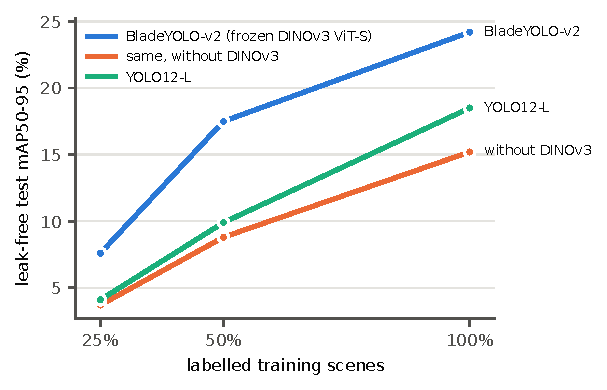
\includegraphics[width=0.92\linewidth]{fig4_dinov3_learning_curve}
\caption{Learning curves with and without frozen DINOv3 on WTBD-group. The modules around DINOv3 do not put the model above stock YOLO12-L.}
\label{fig:curve}
\end{figure}

Without DINOv3, BladeYOLO-v2 equals or trails stock YOLO12-L at every data size. The advantage is therefore the features, not the architecture around them. We first read it as a low-data advantage; the 50\% and 100\% runs corrected that, since the absolute gain does not shrink with data. Only the relative gain does, from $2.0\times$ to $1.6\times$. Labelled scenes still pay throughout: the learning curve has not flattened at 100\%. This claim concerns our components. BladeYOLO's exact style-injection, WTConv and Cross-Mamba modules were reimplemented only before our code audit, so we make no claim about them.

\textbf{Backbone size at 25\%} (Table~\ref{tab:backbone}). A larger frozen backbone helps up to ViT-B, and ViT-L adds nothing further. This is why RF-DETR-FP uses ViT-B.

\begin{table}[!t]
\centering
\caption{Frozen DINOv3 size at 25\% of WTBD-group scenes: test scores by Ultralytics \texttt{val}, per seed and mean; differences by scene bootstrap, \mcoco points. \hlnote{}}
\label{tab:backbone}
\scriptsize
\setlength{\tabcolsep}{1.8pt}
\begin{tabularx}{\linewidth}{@{}l X c c l@{}}
\toprule
Backbone & Per seed (50/50:95) & Mean 50 & Mean 50:95 & $\Delta$\mcoco [95\% CI] \\
\midrule
none (2) & 11.4/4.4, 8.1/3.1 & 9.8 & 3.8 & none$-$S: $-3.9$ \ci{-10.1}{-2.5} \\
ViT-S/16 (3) & 23.2/8.2, 22.4/8.7, 18.4/6.8 & 21.3 & 7.9 & \\
ViT-B/16 (2) & 25.2/10.2, 28.3/11.6 & \second{26.8} & \second{10.9} & B$-$S: $+2.8$ \ci{+0.4}{+9.6} \\
ViT-L/16 (2) & 33.7/11.5, 30.1/10.9 & \best{31.9} & \best{11.2} & L$-$B: $+0.3$ \ci{-4.0}{+3.1} \\
\bottomrule
\end{tabularx}
\end{table}

\textbf{Fine-tuned against frozen foundation features, 25\% labels, same subsets (V1).} RF-DETR-M beats BladeYOLO-v2 ViT-B by $+7.3$ \ci{+2.3}{+11.9} \mcoco (seed 0) and $+8.3$ \ci{+4.5}{+15.0} (seed 1), and it is positive on 4 of 4 subsets at each seed. As a controlled comparison, freezing RF-DETR's own encoder lowers test \mcoco from 18.9 to 12.3 on WTBD and from 13.2 to 8.7 on WTBlade. Input resolution (G24) adds $+1.0$ from 576 to 768\,px on WTBD ($P=0.958$) and $-0.1$ on WTBlade, whose frames are natively 640\,px.

\subsection{Training Behaviour}
Fig.~\ref{fig:training} shows validation curves from the final-phase runs. RF-DETR peaks early and then drifts down, which is why EMA checkpoint selection matters. In contrast, YOLO12-L on WTBlade-group rises almost linearly until about epoch 43 of 50, so its row may understate it. Fig.~\ref{fig:examples} shows training and validation batches, and Fig.~\ref{fig:diagnostics} confusion matrices and a PR curve. In the matrices, columns are true classes. The bottom row shows missed labels (crack 18\% on WTBD-group and 27\% on WTBlade-group for YOLO12-L), and the right column shows where false positives go. The strongest confusions involve rare classes: YOLO12-L calls 54\% of thunderstrike labels craze on WTBD-group test.

\begin{figure*}[!t]
\centering
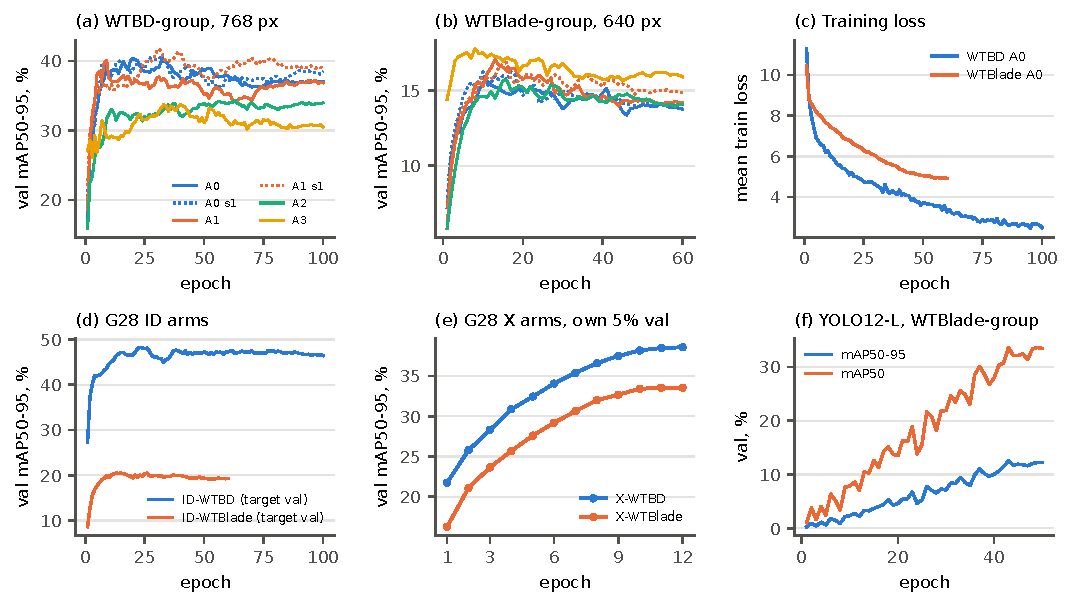
\includegraphics[width=\textwidth]{fig15_training_curves}
\caption{Training records. (a, b) Validation \mcoco of the G27 arms; dotted lines are seed 1. (c) Training loss of A0. (d) G28 ID arms on target validation. (e) G28 X arms on their own held-out 5\%, not comparable with (d) since the images differ. (f) YOLO12-L on WTBlade-group.}
\label{fig:training}
\end{figure*}

\begin{figure*}[!t]
\centering
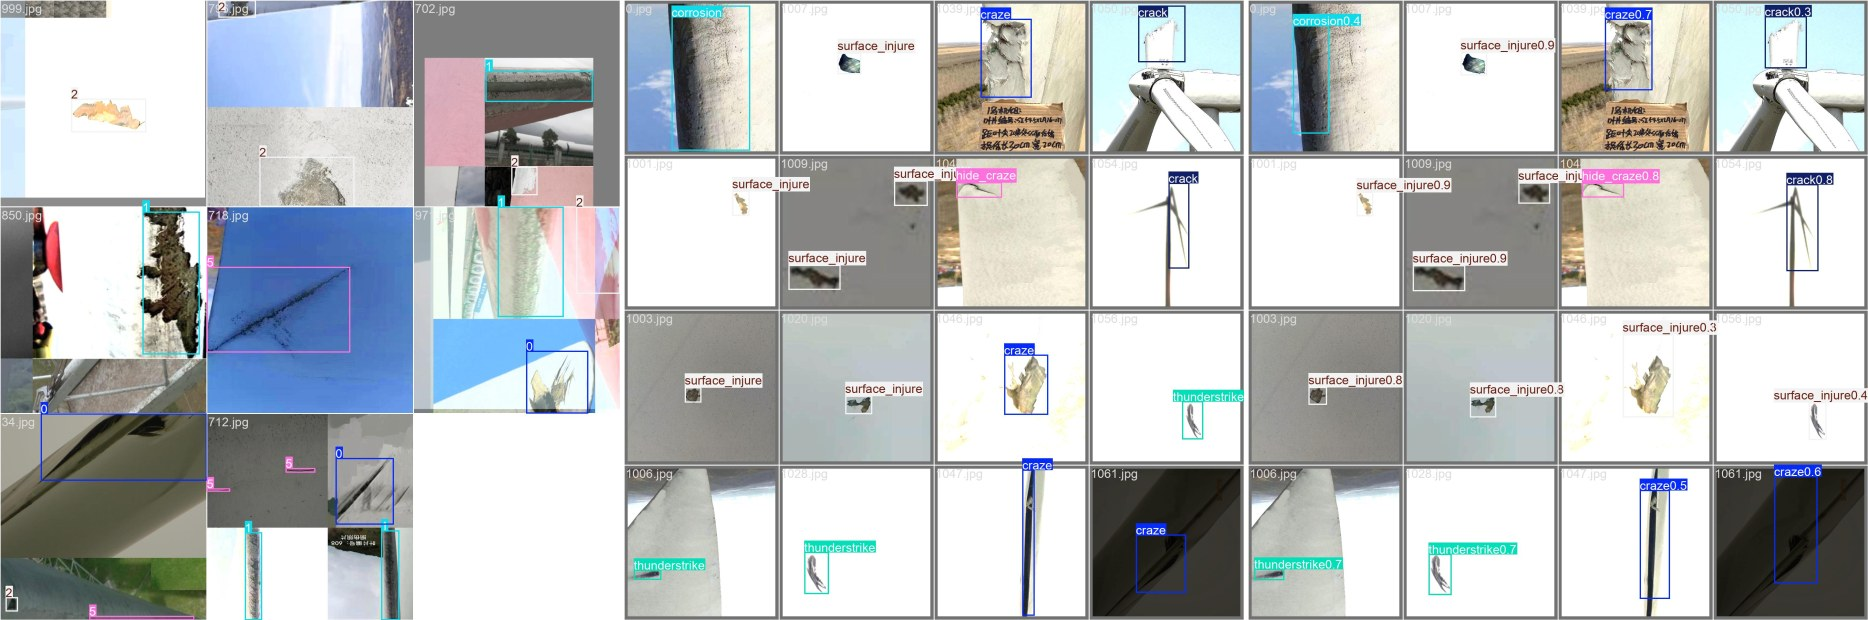
\includegraphics[width=\textwidth]{fig26_training_examples}
\caption{BladeYOLO-v2 on WTBD-group, from the training run. Left: a training batch after mosaic and flips. Middle: a validation batch with its labels. Right: the same batch with predictions.}
\label{fig:examples}
\end{figure*}

\begin{figure}[!t]
\centering
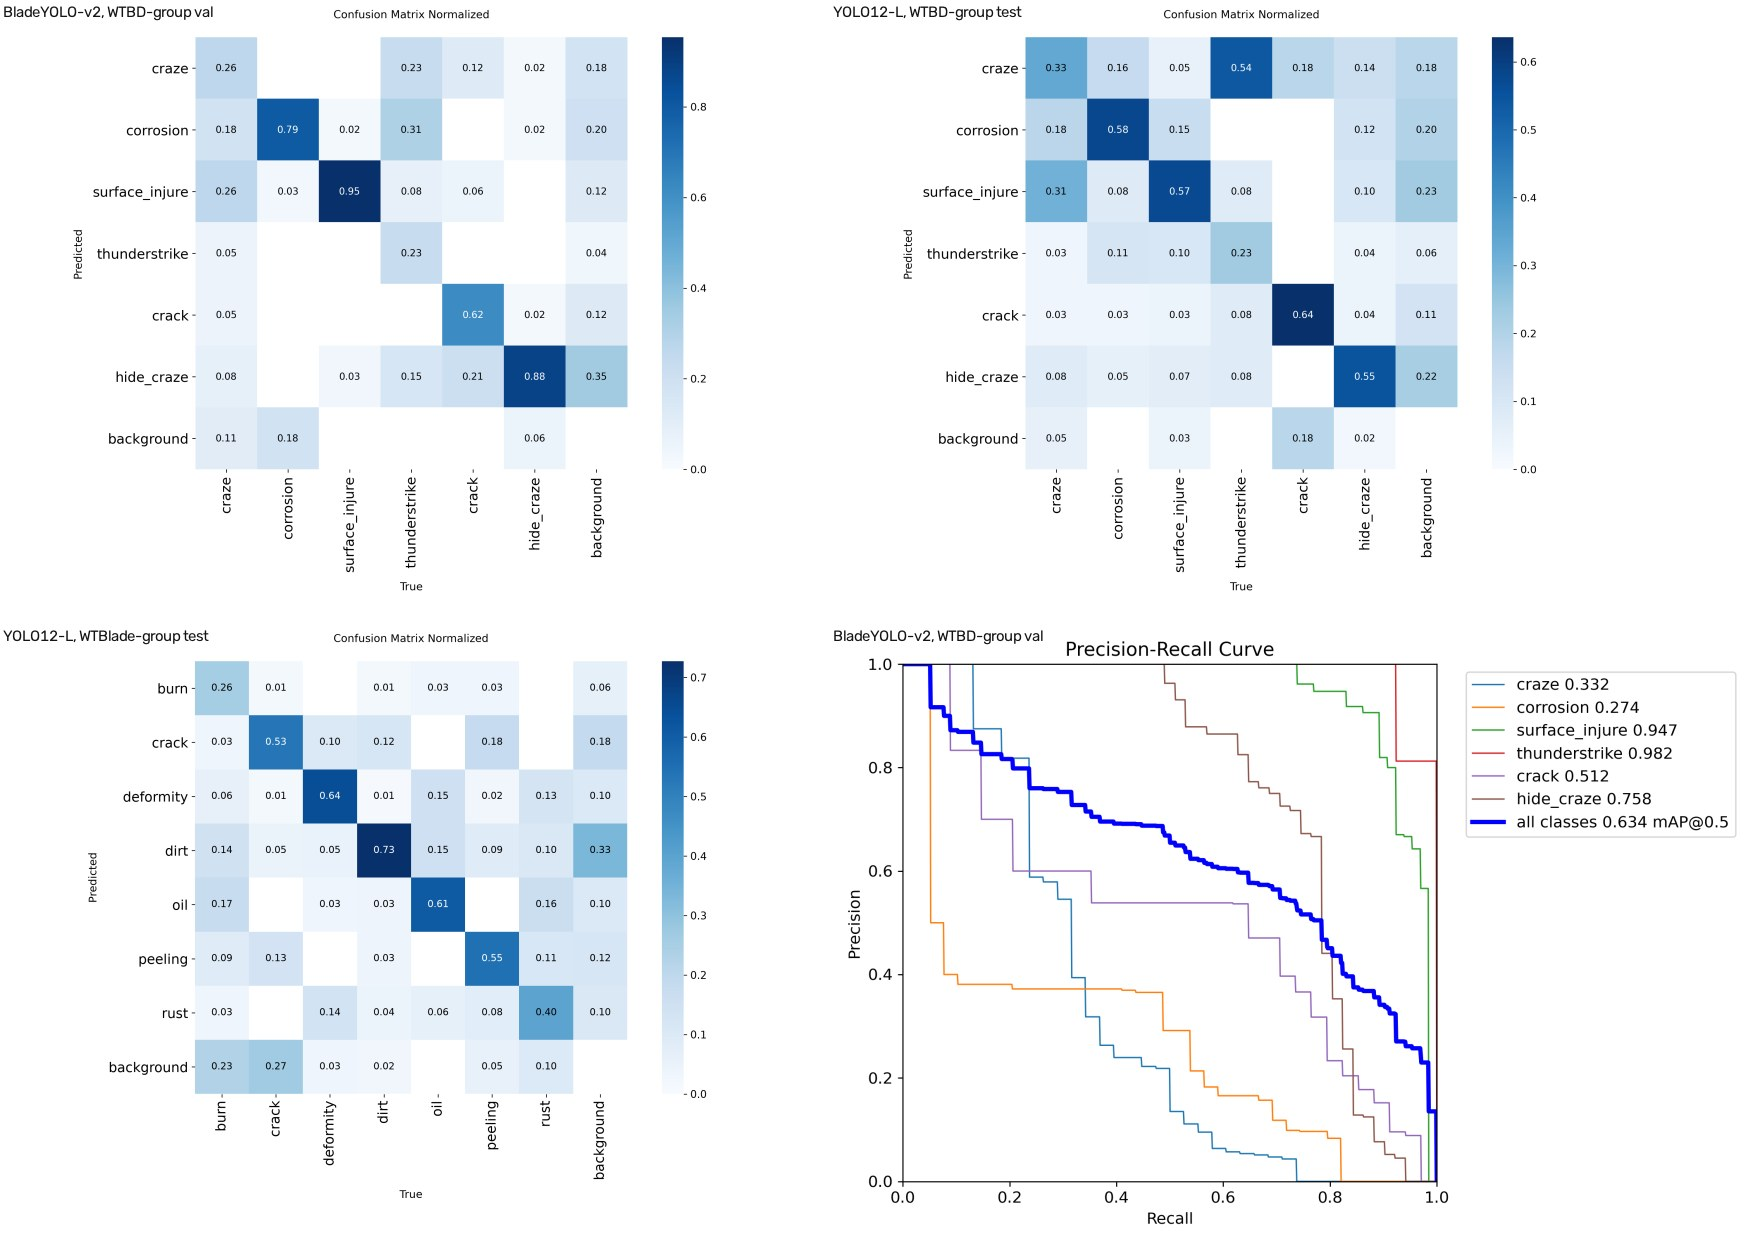
\includegraphics[width=\linewidth]{fig27_diagnostics}
\caption{Diagnostics. Normalised confusion matrices: BladeYOLO-v2 on WTBD-group validation, YOLO12-L on WTBD-group test and YOLO12-L on WTBlade-group test. Bottom right: PR curves by class of BladeYOLO-v2 on WTBD-group validation.}
\label{fig:diagnostics}
\end{figure}

\section{Why Leak-Free Scores Are Low}
\label{sec:why}

\subsection{The Annotators Against Themselves}
WTBD's augmented copies were annotated independently, so aligned copies of an image give accidental repeated labels. For every verified pair of the same surface we project each label through the estimated transform. The transform is a flip-aware ORB + RANSAC similarity with at least 25 inliers, and at least 8 of them inside the box. We then classify the label as \emph{agree} (same class, IoU~$\geq0.5$), \emph{class conflict}, \emph{split}, \emph{loose} or \emph{missing}. Fig.~\ref{fig:ambiguity} shows examples, and Table~\ref{tab:selfconsistency} gives the rates.

\begin{figure*}[!t]
\centering
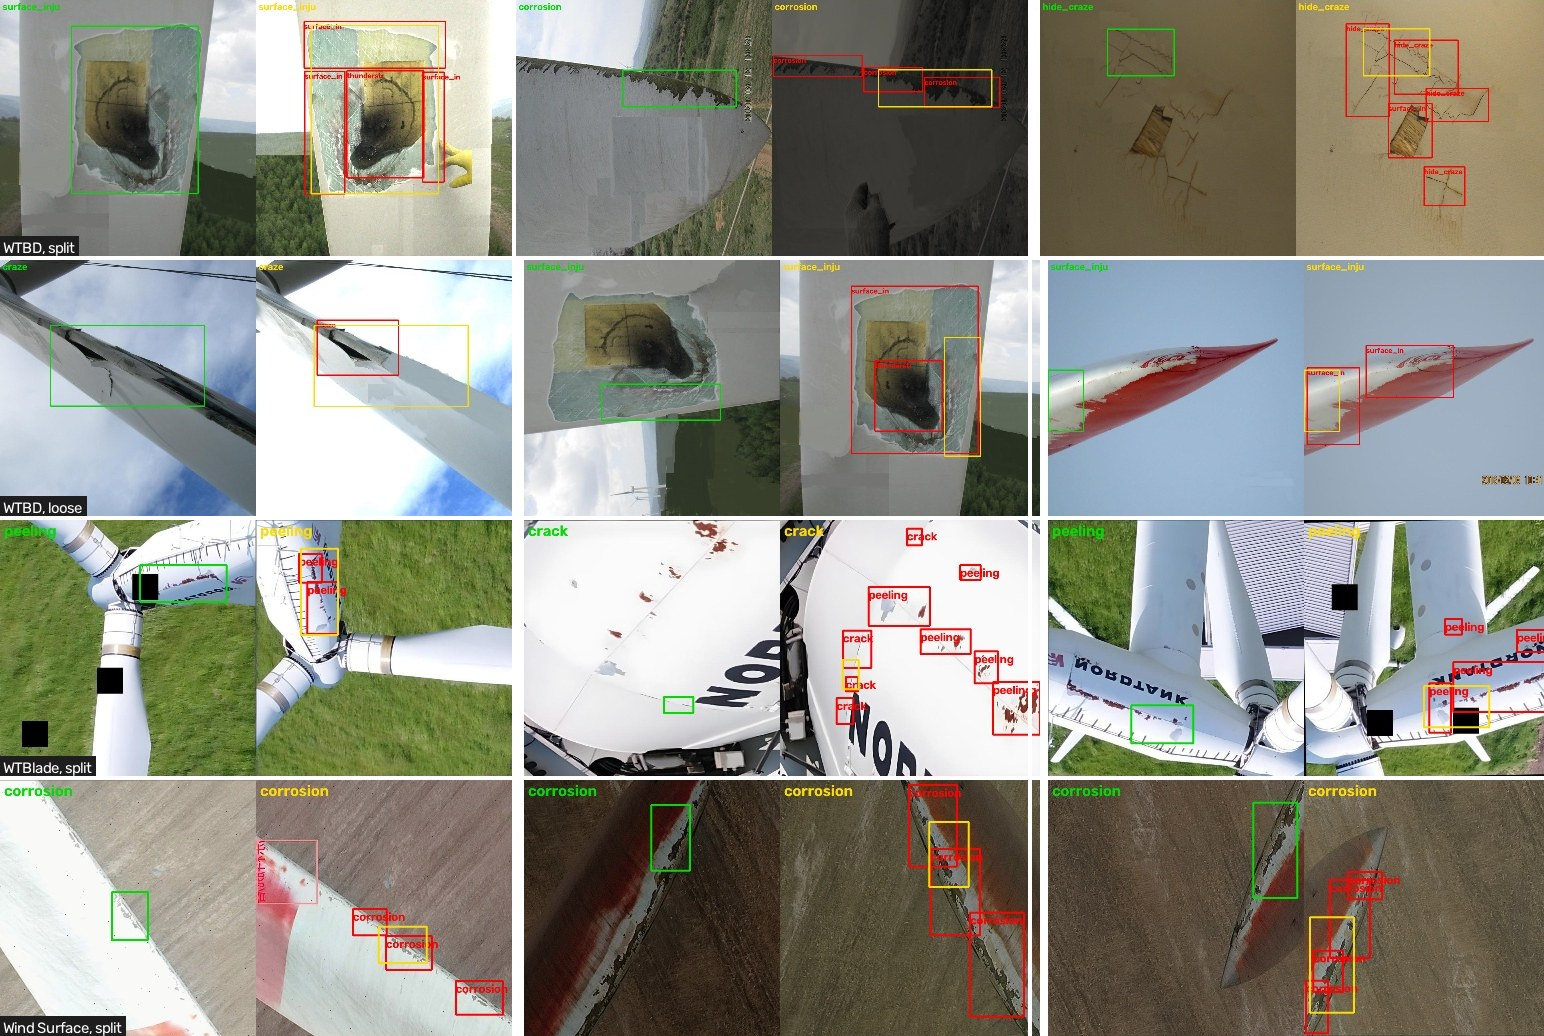
\includegraphics[width=0.86\textwidth]{fig11_label_ambiguity}
\caption{Annotation ambiguity on aligned copies. In each pair, left: a label (green); right: its exact projection (yellow) and what the copy's annotator drew (red). Top two rows: WTBD. Third row: WTBlade-Defect. Bottom row: Wind Surface. The disagreement is about extent and about how a defect is cut into boxes, not about the class. ``NORDTANK'' is legible in the third row.}
\label{fig:ambiguity}
\end{figure*}

\begin{table}[!t]
\centering
\caption{Label self-consistency on axis-aligned copies of the same image (rotation within 3$^\circ$ of a multiple of 90$^\circ$, flips included), where boxes map to boxes and every difference is an annotation difference. Rotated copies and other views agree less, but those strata also include geometric effects.}
\label{tab:selfconsistency}
\footnotesize
\setlength{\tabcolsep}{2.2pt}
\begin{tabular}{@{}l r r r r r r r r@{}}
\toprule
Dataset & Labels & Agree & Split & Loose & Miss & Class & Rot. & Other \\
\midrule
WTBD & 2{,}965 & \textbf{87.3} & 4.6 & 6.7 & 1.5 & 0 & 77.9 & 64.1 \\
WTBlade & 42{,}812 & \textbf{86.0} & 2.5 & 8.2 & 3.1 & 91 & 80.7 & 59.8 \\
Wind Surf. & 10{,}261 & \textbf{83.8} & 9.2 & 5.9 & 1.1 & 0 & (18) & 44.2 \\
\bottomrule
\end{tabular}
\tabnote{Percent of labels, except \emph{Class}: number of class conflicts (0.2\% on WTBlade). \emph{Rot.}: agreement on rotated copies; \emph{Other}: on other views of the surface.}
\end{table}

So 13--16\% of labels disagree with an exactly aligned copy in all three datasets, including one that was double-annotated ($\kappa=0.897$~\cite{wtbd}). Almost none of the disagreement is about class. The amorphous classes are the least consistent (Fig.~\ref{fig:agreement}). Counts are per label occurrence, and they concentrate in a few heavily duplicated scenes. On WTBlade the ``missing'' rate is mostly a matching artefact of rotating rotors in video (1.1\% without dirt). Most of its 91 class conflicts are pasted synthetic patches, labelled peeling in one copy and crack in another.

\begin{figure}[!t]
\centering
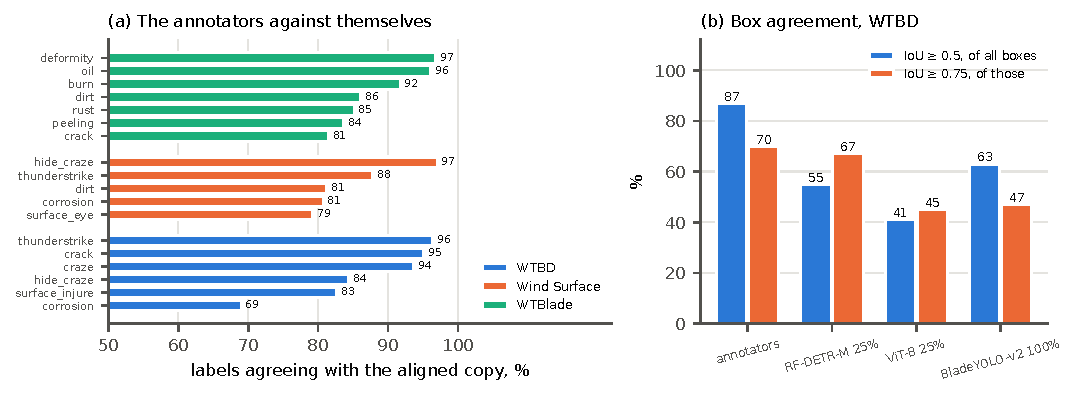
\includegraphics[width=\linewidth]{fig12_label_agreement}
\caption{(a) Per-class agreement on aligned copies. (b) Box agreement on WTBD: how often an independent annotator's box, or a detector's best box, reaches IoU 0.5, and of those, how many reach 0.75 (confidence $\geq$0.1 for detectors). RF-DETR-M at 25\% labels matches the annotators on extent once it finds a defect (0.67 against 0.70; median IoU 0.83 for both).}
\label{fig:agreement}
\end{figure}

\subsection{Box Granularity}
On WTBD-group, tolerant \apfifty exceeds standard \apfifty by $+11.9$ for BladeYOLO-v2 (56.1 to 68.0) and by $+12.4$ for YOLO12-L (40.0 to 52.4). The most striking class is craze, which rises from 9.9 to 66.1. All 15 craze test images are rotated, flipped or recoloured copies of one long leading-edge split, annotated as 2--3 segment boxes (Fig.~\ref{fig:craze}). The same effect holds for RF-DETR scored with classes merged: \apfifty rises from 66.1 to 79.7 on WTBD-group and from 50.1 to 61.2 on WTBlade-group. Table~\ref{tab:granularity} gives the per-class view.

\begin{figure}[!t]
\centering
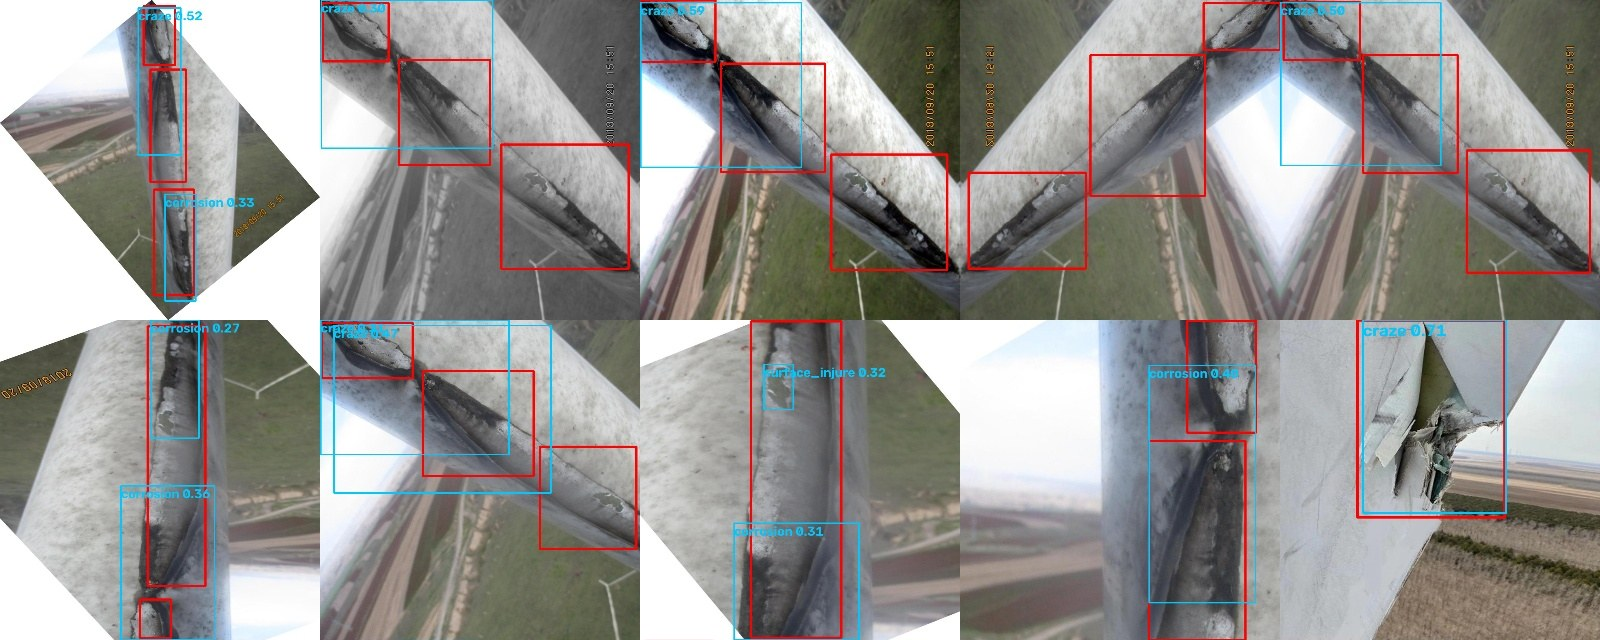
\includegraphics[width=\linewidth]{fig13_craze_scene}
\caption{All 15 WTBD-group craze test images come from one scene. Red: labels, split into segments by the annotator. Blue: BladeYOLO-v2 predictions. The model often draws one box where the label has several, which counts as an error at IoU 0.5 and explains most of the ``craze failure''.}
\label{fig:craze}
\end{figure}

\begin{table}[!t]
\centering
\caption{Three box scores on WTBD-group test, in percent (500 scene replicates). Per class: BladeYOLO-v2. The official-minus-group gap shrinks as the metric becomes split-invariant (BladeYOLO-v2: $+25.4$, $+20.9$, $+16.8$). \best{Red bold}: better model on each split.}
\label{tab:granularity}
\scriptsize
\setlength{\tabcolsep}{1.5pt}
\begin{tabularx}{\linewidth}{@{}X l l l@{}}
\toprule
& Std.\ \apfifty & Tol.\ \apfifty & Region AP \\
\midrule
BYv2, group & \best{56.1} \ci{48.3}{79.1} & \best{68.0} \ci{60.4}{83.1} & \best{60.3} \ci{55.2}{74.3} \\
YOLO12-L, group & 40.0 \ci{33.9}{67.8} & 52.4 \ci{46.5}{74.0} & 44.1 \ci{40.2}{59.2} \\
difference & $+16.1$ \ci{+2.3}{+28.4} & $+15.6$ \ci{+0.1}{+23.7} & $\mathbf{+16.2}$ \ci{+7.7}{+23.6} \\
BYv2, official & \best{81.5} & \best{88.9} & \best{77.1} \\
YOLO12-L, official & 69.0 & 80.0 & 66.6 \\
\midrule
craze & 9.9 & \textbf{66.1} & 42.7 \\
corrosion & 62.6 & 67.6 & 68.4 \\
surface\_injure & 75.9 & 81.6 & 68.9 \\
thunderstrike & 100.0 & 100.0 & 68.2 \\
crack & 35.2 & 35.6 & 49.1 \\
hide\_craze & 53.0 & 56.8 & 64.5 \\
\bottomrule
\end{tabularx}
\end{table}

Two limits apply. First, we hypothesised that part of the leakage inflation is memorised box splitting, and tested it. The tolerant gain is not smaller on test images with a training twin, so the hypothesis is not supported. Second, training a detector to tolerate splitting does not help overall. Blanket split-tolerant training is not an improvement (tolerant \apfifty $+1.5$ \ci{-11.1}{+6.4}). Class-selective tolerance raises corrosion by $+9.3$ \ci{-0.3}{+24.6}, while the mean moves by $-0.4$. The ambiguity therefore limits what can be measured more than what can be trained away.

\textbf{Annotators as a ceiling.} Corrosion copies agree on only 69\% of labels, and models score near that (BladeYOLO-v2 \apfifty 54--63), so further corrosion ``improvement'' is largely unmeasurable with these labels. Crack copies agree on 95\% while the YOLO family scores 35--39, so crack is a genuine model weakness there.

\subsection{Subset Luck}
At a fixed budget of 25\% of scenes, which scenes are labelled matters more than any model effect we measured (Fig.~\ref{fig:luck}). Across 8 random draws with the same model, recipe and seed, ViT-B test \mcoco spans 9.0--19.6 ($\times2.2$); without DINOv3 it spans 2.6--7.2. The DINOv3 gain holds on 8 of 8 draws ($+7.1$ \ci{+5.1}{+12.6}), and draw quality carries over between models (Spearman $\rho=0.71$). Yet no label-free subset property we tested predicts it (H7, G16, H20). Label-free scene selection by patch coverage beats random by $+5.2$ \ci{+1.9}{+10.5}. It does not separate from FreeSel~\cite{freesel}, however: $+2.1$ \ci{-1.2}{+9.1}, $P=0.917$, with validation pointing the other way. Table~\ref{tab:selection} gives the selection runs at the 25\% budget. Selecting by class balance does worst of the five arms, which suggests that \emph{which} scenes are labelled matters more than matching class counts.

\begin{table}[!t]
\centering
\caption{Selection of which 25\% of WTBD-group scenes to label: 18 ViT-B runs at the same budget, training seed 0. Random draws per run: 11.2, 13.5, 11.8, 12.3, 9.0, 10.0, 12.4, 19.6. \hlnote{}}
\label{tab:selection}
\footnotesize
\setlength{\tabcolsep}{2.4pt}
\begin{tabularx}{\linewidth}{@{}X r r r l@{}}
\toprule
Arm (runs) & Test \mfifty & Test \mcoco & Val \mcoco & Rank (test/val) \\
\midrule
Patch coverage, label-free (4) & \second{40.6} & \best{17.7} & 23.6 & 2/9, 3/9 \\
FreeSel-224 (2) & \best{42.9} & \second{15.6} & \best{27.1} & 2/9, 1/9 \\
FreeSel-640 (2) & 34.4 & 14.5 & \second{26.6} & 2/9, 2/9 \\
Random (8) & 31.3 & 12.5 & 21.6 & \\
Class-matched, uses labels (2) & 25.3 & 10.4 & 19.7 & 7/9, 7/9 \\
\bottomrule
\end{tabularx}
\end{table}

\begin{figure}[!t]
\centering
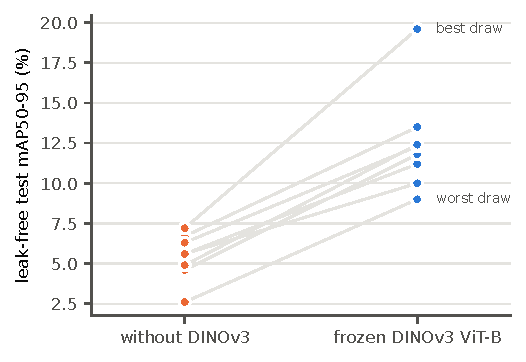
\includegraphics[width=0.9\linewidth]{fig5_subset_luck}
\caption{Subset luck: test \mcoco across random 25\% scene draws, same model, recipe and seed.}
\label{fig:luck}
\end{figure}

\subsection{Error Anatomy}
\label{sec:anatomy}
Scarce labels fail differently by detector family (Fig.~\ref{fig:anatomy}, in the style of TIDE~\cite{tide}). For each test box we ask whether a same-class box at IoU~$\geq0.5$ is among the outputs, and how it is scored. Table~\ref{tab:anatomy} gives the numbers, and Table~\ref{tab:ceiling} the extent comparison.

\begin{figure}[!t]
\centering
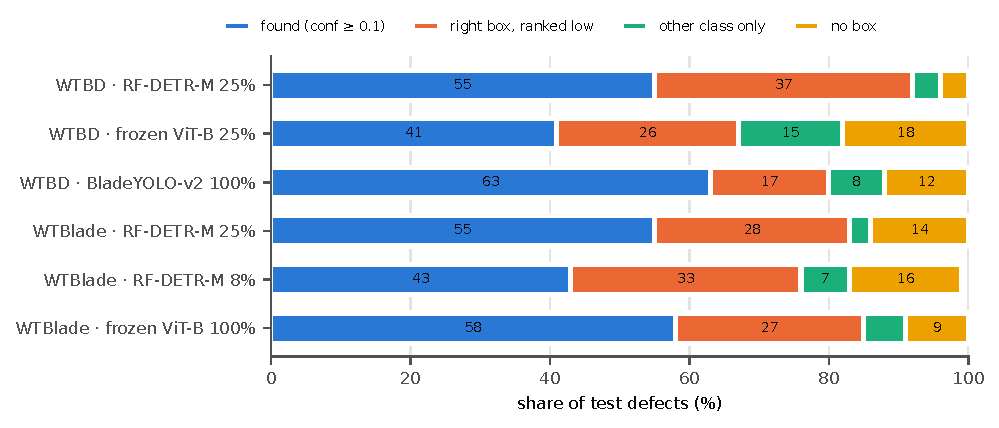
\includegraphics[width=\linewidth]{fig6_error_anatomy}
\caption{Error anatomy. Hit: a same-class box at IoU $\geq$0.5 with confidence $\geq$0.1. Ranked low: such a box exists only below 0.1. Other class: only other-class boxes at IoU $\geq$0.5. No box: nothing at IoU $\geq$0.5.}
\label{fig:anatomy}
\end{figure}

\begin{table}[!t]
\centering
\caption{Error anatomy as a share of test boxes. Candidate recall = hit + ranked low. YOLO-family runs keep fewer boxes after NMS (about 50--80 per image) than RF-DETR (300), so recall within each image's top 50 boxes is also given. \hlnote{} (within each dataset; for Other and None lower is better)}
\label{tab:anatomy}
\footnotesize
\setlength{\tabcolsep}{2pt}
\begin{tabularx}{\linewidth}{@{}X r r r r r r@{}}
\toprule
Detector & Hit & Low & Other & None & Cand. & Top 50 \\
\midrule
\multicolumn{7}{@{}l}{\textit{WTBD-group}} \\
RF-DETR-M 25\% (4 subsets) & \second{0.55} & 0.37 & \best{0.04} & \best{0.04} & \best{0.92} & \best{0.81} \\
ViT-B 25\% (4 subsets) & 0.41 & 0.26 & 0.15 & 0.18 & 0.67 & 0.66 \\
BladeYOLO-v2 100\% (2 seeds) & \best{0.63} & 0.17 & \second{0.08} & \second{0.12} & \second{0.80} & \second{0.80} \\
\multicolumn{7}{@{}l}{\textit{WTBlade-group}} \\
RF-DETR-M 25\% (4 subsets) & \second{0.55} & 0.28 & \best{0.03} & \second{0.14} & \second{0.83} & \second{0.72} \\
RF-DETR-M 8\% (4 subsets) & 0.43 & 0.33 & 0.07 & 0.16 & 0.77 & 0.62 \\
ViT-B 100\% & \best{0.58} & 0.27 & \second{0.06} & \best{0.09} & \best{0.85} & \best{0.81} \\
\bottomrule
\end{tabularx}
\end{table}

\begin{table}[!t]
\centering
\caption{Box extent against the annotator ceiling on WTBD: the same-class IoU of a label with its copy, or of the best prediction with confidence $\geq0.1$, per test box. \hlnote{} (among detectors; annotators are the reference)}
\label{tab:ceiling}
\footnotesize
\setlength{\tabcolsep}{2.2pt}
\begin{tabularx}{\linewidth}{@{}X r r r r r@{}}
\toprule
Source & Boxes & $\geq$0.5 & of those $\geq$0.75 & median & $\geq$0.75 \\
\midrule
Annotators, all copies & 2{,}965 & 0.87 & 0.70 & 0.83 & 0.61 \\
Annotators, test copies & 392 & 0.91 & 0.75 & 0.84 & 0.68 \\
RF-DETR-M 25\% & 940 & \second{0.55} & \best{0.67} & \best{0.83} & \best{0.37} \\
ViT-B 25\% & 940 & 0.41 & 0.45 & 0.73 & 0.19 \\
BladeYOLO-v2 100\% & 235 & \best{0.63} & \second{0.47} & \second{0.74} & \second{0.29} \\
\bottomrule
\end{tabularx}
\end{table}

\begin{itemize}
\item \textbf{RF-DETR at 25\% labels proposes the right box for most defects.} Candidate recall is 0.92 on WTBD, above BladeYOLO-v2 at 100\% (0.80), and 0.83 on WTBlade. Its deficit is scoring: 37\% of WTBD test defects have a correct box scored below 0.1. Once it finds a defect, its box matches the label as well as a second annotator's does.
\item \textbf{On WTBD the rare classes are confused.} Crack is missed or mislabelled, and thunderstrike is found under other classes (54\% located as another class, over 4 subsets). On WTBlade, 43--49\% of crack boxes lack a same-class box at IoU~$\geq0.5$ at every budget (RF-DETR 8\%: 0.47; 25\%: 0.49; ViT-B 100\%: 0.43), so this is not a label-budget problem. Misses concentrate on small boxes (1.00 below 16\,px, 0.65 below 32\,px, 0.22 above 64\,px). Among near-misses, the largest share is shifted boxes (44\%), not split ones.
\item \textbf{Not resolution, on WTBD.} Median defect short sides at 640\,px are 62--148\,px by class.
\end{itemize}

\section{Leave-One-Dataset-Out: Data Volume Does Not Replace Target Labels}
\label{sec:lodo}

If the label count were the bottleneck, pooling every other blade dataset should help. G28 tests this directly. It was pre-registered before any pool was built or any run started.

\subsection{Design}
For each target $T$, two class-agnostic RF-DETR-M arms (640\,px, cosine, seed 0) are scored on $T$'s test set:
\begin{itemize}
\item \textbf{ID-$T$}: trained on $T$'s group training split (WTBD 100 epochs, WTBlade 60).
\item \textbf{X-$T$}: trained for 12 epochs on every other source, twin-free against \emph{all} of $T$. Selection uses a held-out 5\% of X-$T$'s own images~\cite{domainbed}, so $T$ is never seen, not even for selection.
\end{itemize}
Every image of $T$ is an evaluation key for the twin rule: the same file, DINOv2 cosine $\geq0.90$, ORB $\geq25$ inliers, pixel correlation $\geq0.97$ over eight orientations, and the closure of all of these. GAN images and images without boxes are dropped. The rule deliberately sits below the audit's twin thresholds (0.93 and 0.99). Earlier versions of this rule, built for the G27 pool, kept 830 pixel twins and then neighbouring video frames; each failure was logged and fixed before any training. Fig.~\ref{fig:pools} shows the result. X-WTBD has 26{,}065 training images (55{,}845 boxes across its train and held-out images), and X-WTBlade has 14{,}405 (27{,}844). Fig.~\ref{fig:poolaudit} shows the closest pairs an independent audit could find. The highest pixel correlation and cosine to any target image are 0.964/0.827 for X-WTBD and 0.970/0.900 for X-WTBlade.

\begin{figure}[!t]
\centering
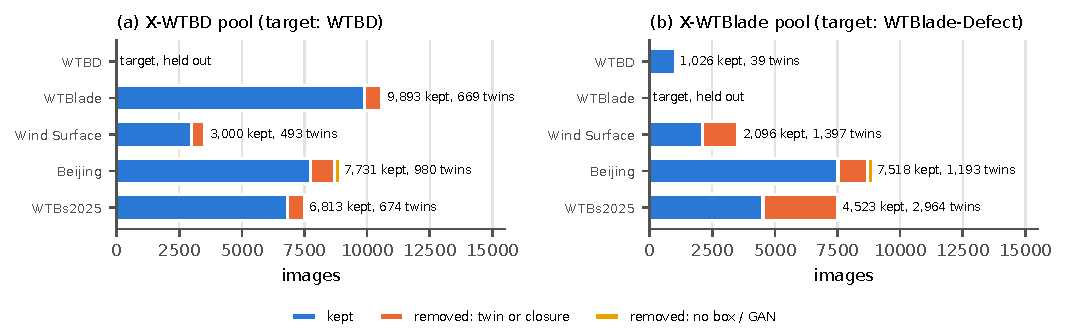
\includegraphics[width=\linewidth]{fig20_pools}
\caption{Composition of the G28 pools: images kept from each source and removed by the twin rule. For X-WTBlade, 2{,}964 WTBs2025 images are removed, since that dataset contains WTBlade-Defect's images.}
\label{fig:pools}
\end{figure}

\begin{figure}[!t]
\centering
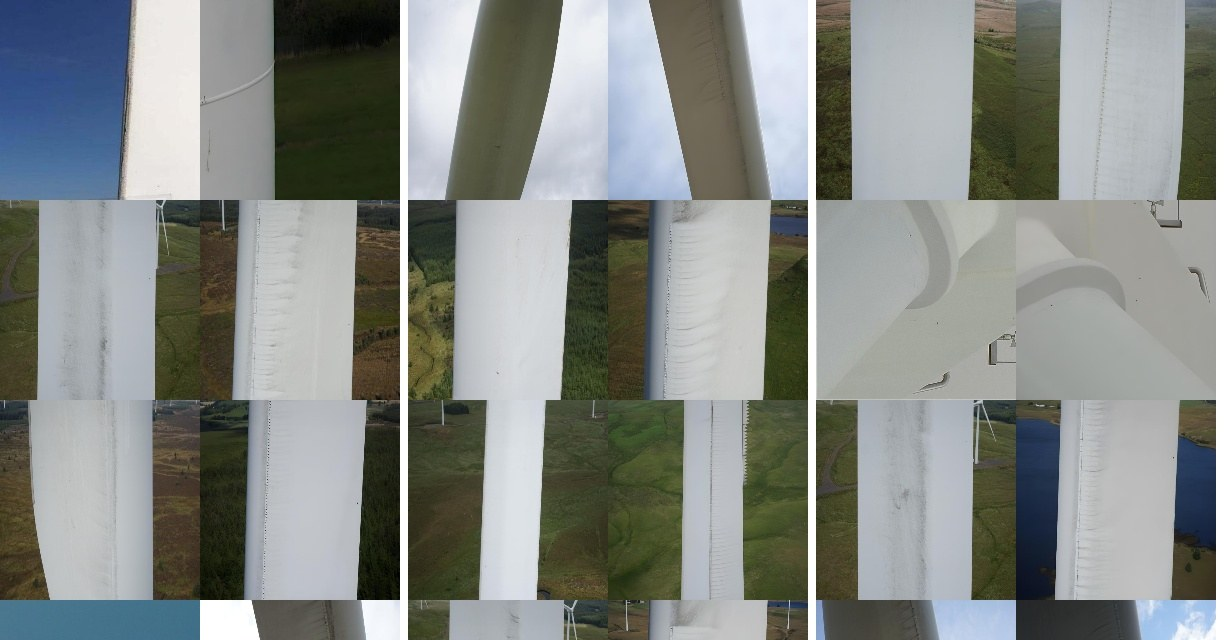
\includegraphics[width=0.9\linewidth]{fig21_pool_audit}
\caption{Independent audit of the X-WTBlade pool: the closest remaining pairs by pixel correlation between a kept pool image and a target image. By eye these are similar blades, not copies. The same physical defect from another flight cannot be excluded without capture metadata.}
\label{fig:poolaudit}
\end{figure}

We define the gaps $G_{\mathrm{std}}=\mathrm{ID}-\mathrm{X}$ in standard \apfifty and $G_{\mathrm{reg}}=\mathrm{ID}-\mathrm{X}$ in region AP, and the \emph{convention share}
\begin{equation}
s = 1 - G_{\mathrm{reg}}/G_{\mathrm{std}},
\label{eq:share}
\end{equation}
the part of the gap that is about how boxes are drawn. The direction counted as alive only if, on \emph{both} targets, X reached at least $0.80\times$ ID in region AP and $s\geq0.5$. Both bars were judgment calls fixed before any number existed.

\subsection{Results}
\begin{table}[!t]
\centering
\caption{G28, class-agnostic, test, scene bootstrap (2{,}000 replicates). \emph{Ref} is G27 A0 (class-aware), scored with classes merged; reported, not decisive. \emph{Trivial} is one box over the whole image. Tol.: tolerant \apfifty; Reg.: region AP. \hlnote{} (within each target)}
\label{tab:g28}
\footnotesize
\setlength{\tabcolsep}{2pt}
\begin{tabularx}{\linewidth}{@{}l X r l r r r@{}}
\toprule
Target & Arm & Train & \apfifty & AP$_{50:95}$ & Tol. & Reg. \\
\midrule
WTBD & ID & 745 & \best{72.9} \ci{57.6}{86.3} & \best{41.9} & \best{84.6} & \best{68.9} \\
 & X & 26{,}065 & \textbf{17.7} \ci{11.9}{28.4} & 6.0 & 24.2 & 43.6 \\
 & ref & 745 & \second{66.1} & \second{40.5} & \second{79.7} & \second{65.9} \\
 & trivial & & 0.0 & & & 14.0 \\
\midrule
WTBlade & ID & 2{,}136 & \best{51.7} \ci{48.0}{58.8} & \best{21.5} & \best{65.1} & \best{68.7} \\
 & X & 14{,}405 & \textbf{2.4} \ci{0.8}{3.5} & 0.5 & 3.2 & 37.6 \\
 & ref & 2{,}136 & \second{50.1} & \second{21.3} & \second{61.2} & \second{68.0} \\
 & trivial & & 1.0 & & & 24.2 \\
\bottomrule
\end{tabularx}
\end{table}

\begin{table}[!t]
\centering
\caption{G28 decision. Bars: ratio $\geq0.80$ and share $\geq0.5$ on both targets. ID $-$ X has $P(>0)=1.000$ on every metric of both targets.}
\label{tab:g28-gap}
\scriptsize
\setlength{\tabcolsep}{2pt}
\begin{tabular}{@{}l r r l l l@{}}
\toprule
Target & Ratio & $s$ & $G_{\mathrm{std}}$ [95\% CI] & $G_{\mathrm{reg}}$ [95\% CI] & Verdict \\
\midrule
WTBD & 0.63 & 0.54 & $+55.2$ \ci{+41.7}{+66.4} & $+25.3$ \ci{+14.4}{+33.9} & dead \\
WTBlade & 0.55 & 0.37 & $+49.3$ \ci{+45.0}{+57.2} & $+31.0$ \ci{+26.8}{+34.6} & dead \\
\bottomrule
\end{tabular}
\end{table}

\begin{figure*}[!t]
\centering
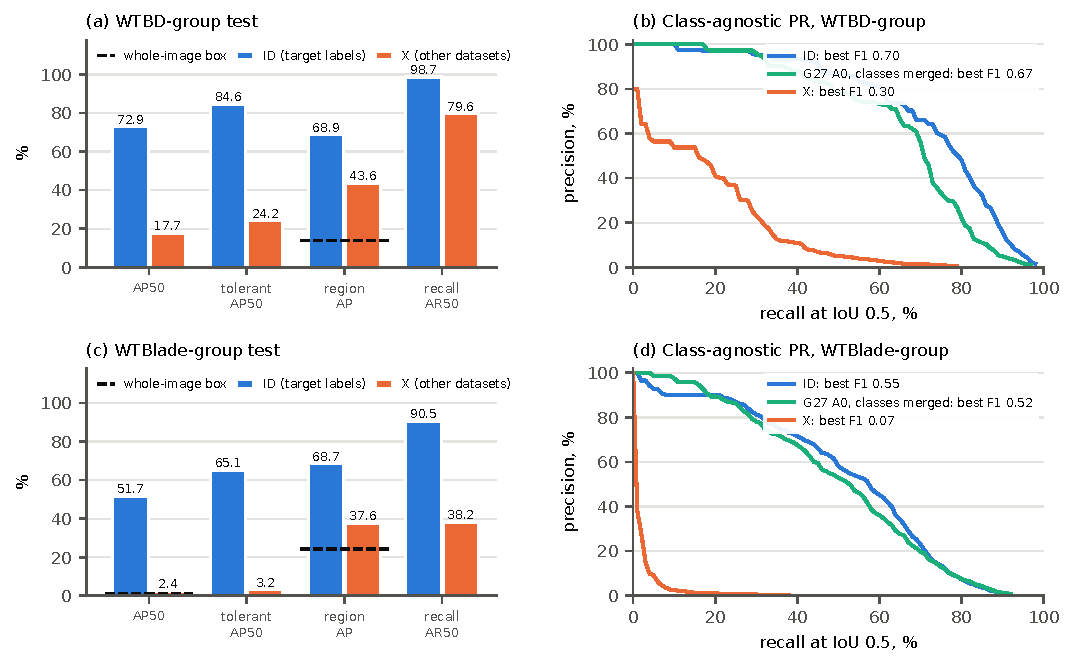
\includegraphics[width=0.96\textwidth]{fig18_g28}
\caption{G28. (a, c) ID and X on target test; dashed lines mark a trivial whole-image detector. (b, d) Class-agnostic precision--recall at IoU 0.5.}
\label{fig:g28}
\end{figure*}

\begin{figure*}[!t]
\centering
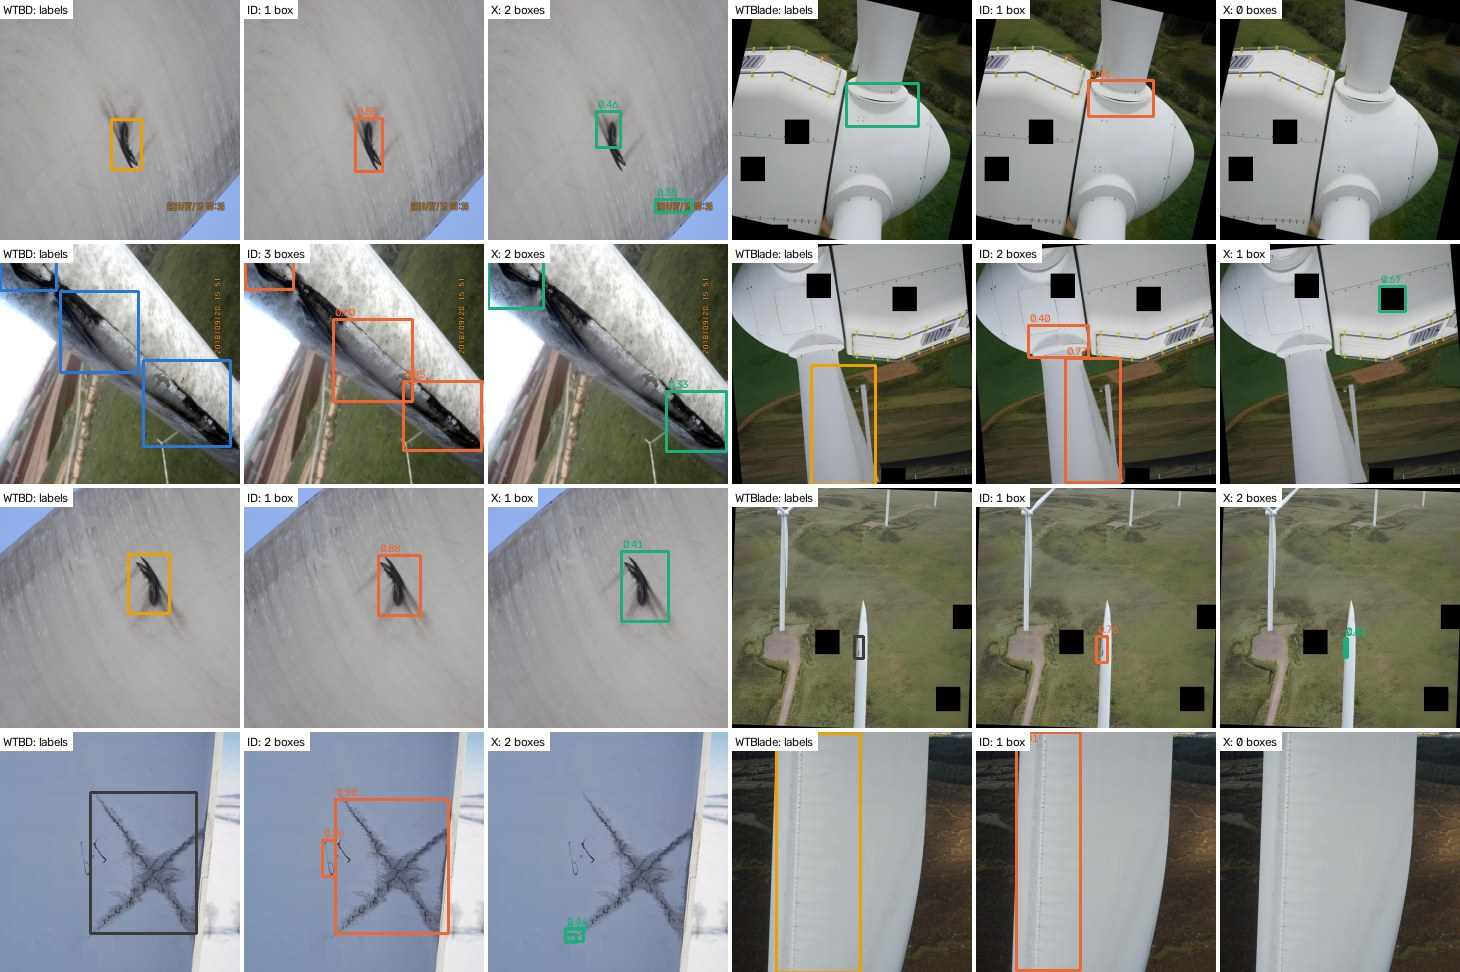
\includegraphics[width=\textwidth]{fig19_predictions}
\caption{Labels, ID and X on random test images (fixed seed), boxes with confidence $\geq$0.3. Left three columns: WTBD-group. Right three: WTBlade-group. X often has the right area or a nearby distractor; it also returns nothing on images where ID is correct.}
\label{fig:predictions}
\end{figure*}

\textbf{The direction fails on both targets} (Tables~\ref{tab:g28}, \ref{tab:g28-gap}; Figs.~\ref{fig:g28}, \ref{fig:predictions}). With 35 times more images from other sources, X still loses to 745 target images by 55 \apfifty points on WTBD-group. The convention explains about half of the gap there and about a third on WTBlade-group; the remainder is a real failure to find the defect. Without the residual pixel-twin images of Fig.~\ref{fig:residual}, the decision is unchanged (ratio 0.64 and 0.56, share 0.55 and 0.39).

\textbf{The model did train.} X-WTBD reached 72.2 \mfifty on its own held-out images at its final epoch. Its region AP is above a trivial detector on both targets (43.6 against 14.0, and 37.6 against 24.2), so it carries information about where defects are. It is not usable as a detector on an unseen dataset, though: X-WTBlade's \apfifty of 2.4 is barely above boxing the whole image (1.0).

\textbf{Why recall and AP disagree on WTBD.} X finds 79.6\% of WTBD labels at IoU 0.5 while scoring 17.7 \apfifty. The reason is that its true boxes rank among many false ones. At recall 10\%, its precision is 54\% against 100\% for ID; at recall 30\% it is 23\% against 95\%. On WTBlade-group, X's precision at recall 10\% is only 3\%, against 90\% for ID. Some false positives are genuine damage of kinds $T$ does not label, so this test is conservative for X.

\textbf{Earlier evidence agrees} (Table~\ref{tab:transfer}). Models trained on one benchmark transfer poorly to the other, and an open-vocabulary foundation detector finds almost nothing without training.

\begin{table}[!t]
\centering
\caption{Generalisation outside one dataset, earlier experiments (BladeYOLO-v2 models; class-agnostic; damage classes only for transfer).}
\label{tab:transfer}
\footnotesize
\begin{tabularx}{\linewidth}{@{}X X@{}}
\toprule
Setting & Result \\
\midrule
WTBlade model on WTBD-group test & \apfifty 5.2 (in-domain 56.3, 58.0); $\Delta$ $-52.5$ \ci{-69.4}{-32.9} \\
WTBD models on WTBlade-group test & \apfifty 4.0, 2.2 (in-domain 47.5); $\Delta$ $-43.9$ \ci{-49.6}{-34.6} \\
Mapped classes across datasets & crack 0.0 both ways; thunderstrike/burn $\leq$7.3 \\
OWLv2~\cite{owlv2}, text queries, no training & \mfifty 3.3 (class-agnostic 5.7); trained on 25\%: 25.0--25.7 \\
OWLv2, few-shot prototypes (25\%) & \mfifty 0.6 (class-agnostic 0.5) \\
\bottomrule
\end{tabularx}
\end{table}

\section{What Did Not Work}
\label{sec:failed}

The leak-free gap motivated many attempts. We report them because a reader should know which common ideas have been tried on these data and how they fared.

\subsection{G27: One Recipe for All Protocols}
Diagnostics said three things: RF-DETR's box extent is at the annotator ceiling, its candidate recall is high, and rare-class scoring is where it loses, with post hoc rescoring closed. G27 therefore changed what the model learns from, with three additions on one pre-registered path:
\begin{itemize}
\item \textbf{CP:} copy-paste~\cite{copypaste} of real boxes from the same training set into classes below the median count (Fig.~\ref{fig:copypaste}).
\item \textbf{D1:} in-domain self-supervised adaptation of RF-DETR's DINOv2 encoder by masked feature distillation~\cite{data2vec}, on a leak-checked pool of 22{,}318 images.
\item \textbf{D2:} a multi-dataset supervised stage 1 on the same pool, with partitioned class slots~\cite{multidataset}.
\end{itemize}
Phase A-1 selected the recipe R on validation (seed 0): the best mean among arms that beat A0 on both datasets. Phase A-2 is the primary test claim on seeds 0 and 1: R $-$ A0 $>0$ on each dataset, with pooled $P(>0)\geq0.95$.

\begin{figure}[!t]
\centering
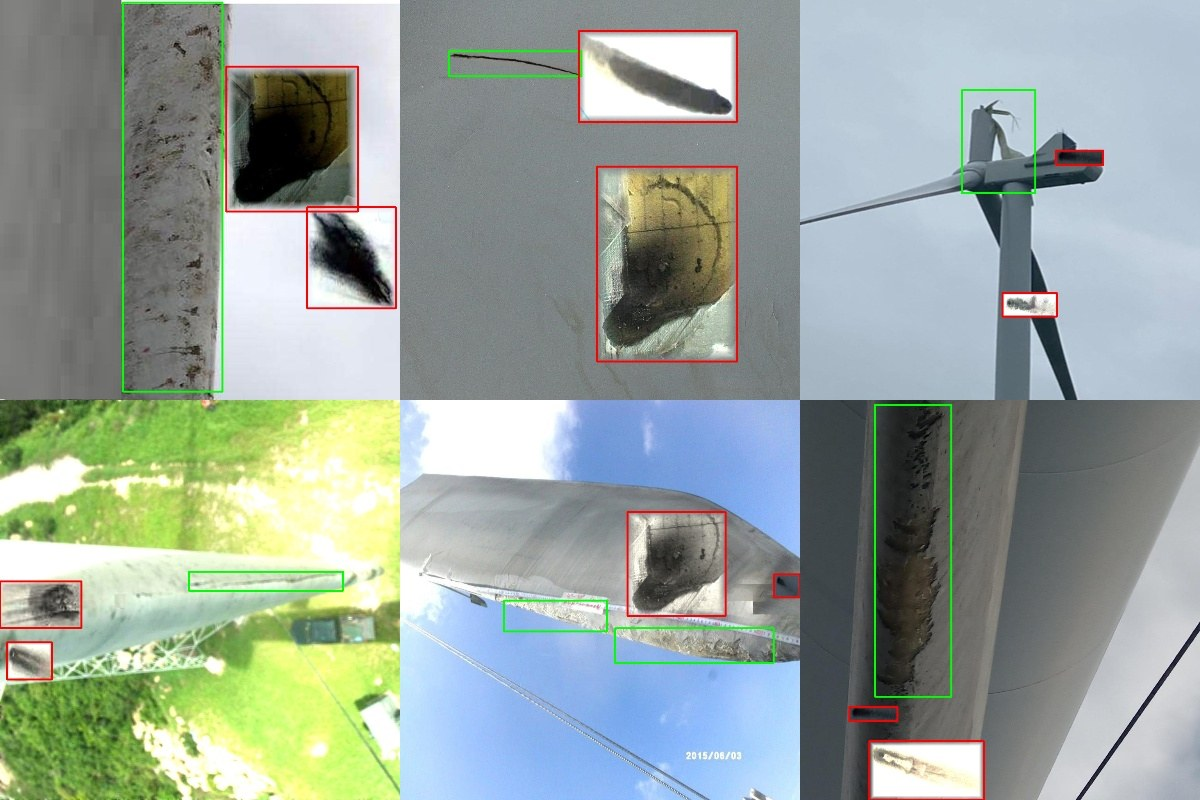
\includegraphics[width=0.9\linewidth]{fig25_cp_check}
\caption{Visual check of copy-paste before training. Some pastes land off the blade where SAM's~\cite{sam2} largest mask includes sky, and box-level pastes carry their source background. These were kept, since A1 $-$ A0 measures the recipe as it ran.}
\label{fig:copypaste}
\end{figure}

\begin{table}[!t]
\centering
\caption{G27 A-2, R = A1 (copy-paste): R $-$ A0, test \mcoco, mean of seeds 0 and 1. The primary claim fails.}
\label{tab:g27}
\footnotesize
\begin{tabular}{@{}l r l r@{}}
\toprule
& R $-$ A0 & 95\% CI & $P(>0)$ \\
\midrule
WTBD-group & $-0.99$ & \ci{-8.6}{+1.2} & 0.193 \\
WTBlade-group & $+0.35$ & \ci{-0.5}{+1.6} & 0.812 \\
mean over datasets & $-0.32$ & \ci{-4.1}{+0.9} & 0.290 \\
\bottomrule
\end{tabular}
\end{table}

\begin{table}[!t]
\centering
\caption{All G27 arms, \mcoco. Validation decided R; test was not used for selection. \hlnote{} (validation, the selection criterion)}
\label{tab:g27val}
\footnotesize
\setlength{\tabcolsep}{2.5pt}
\begin{tabular}{@{}l r l r l@{}}
\toprule
& \multicolumn{2}{c}{WTBD-group} & \multicolumn{2}{c}{WTBlade-group} \\
\cmidrule(lr){2-3}\cmidrule(l){4-5}
Arm & val s0 & test s0/s1 & val s0 & test s0/s1 \\
\midrule
A0 plain & \second{40.11} & 33.2/32.2 & 15.68 & 16.2/16.9 \\
A1 + CP & \best{40.15} & 30.7/32.7 & \second{17.10} & 17.3/16.5 \\
A2 + CP + D1 & 34.2 & 27.4/-- & 15.6 & 16.1/-- \\
A3 + CP + D2 & 33.4 & 33.2/-- & \best{17.7} & 16.6/-- \\
\bottomrule
\end{tabular}
\end{table}

\begin{figure}[!t]
\centering
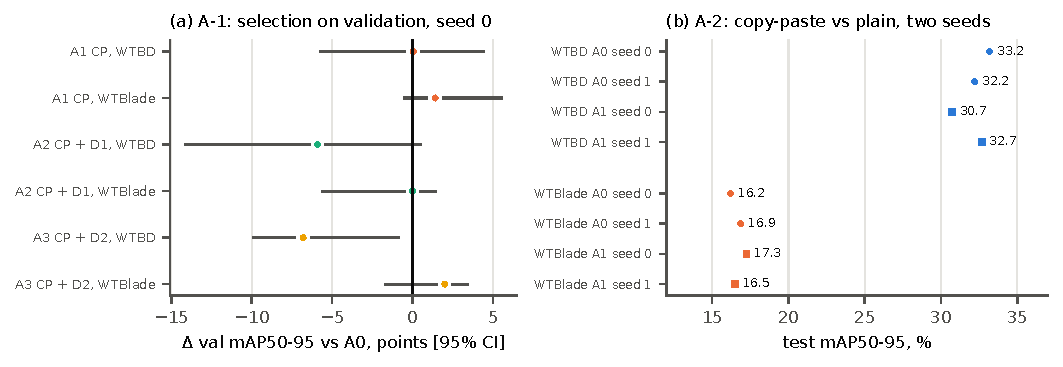
\includegraphics[width=\linewidth]{fig16_g27}
\caption{G27. (a) A-1, validation deltas against A0, seed 0. (b) A-2, test by seed: the seed swing is as large as the effect.}
\label{fig:g27}
\end{figure}

R $=$ A1 was chosen by $+0.04$ points on WTBD-group validation, smaller than A0's own seed-to-seed difference on validation (Tables~\ref{tab:g27}, \ref{tab:g27val}; Fig.~\ref{fig:g27}). Without the residual pixel-twin images, R $-$ A0 is $-1.01$ on WTBD-group and $+0.40$ on WTBlade-group, so the conclusion is unchanged. D1 and D2 were rejected on A-1 ($-5.9$ and $-6.8$ points against A1 on WTBD validation). A post hoc check found that D1 halved the effective rank of the encoder's last stage (257 to 135), a partial dimensional collapse. This finding motivated keeping the prior frozen in RF-DETR-FP. A seed swing of up to 2 points on these test sets (A1 on WTBD: 30.7 and 32.7) sets the smallest effect that can be claimed.

\subsection{Semi-Supervised Learning}
Label budgets suggested semi-supervision, and it took three rounds to rule out (Table~\ref{tab:ssl}). The idea was distinctive: drone inspection produces overlapping real views of the same surface, which our audit registers with verified transforms (about 4{,}000 WTBD and 70{,}000 WTBlade pairs). A teacher's detections on one view can be mapped into another and used as pseudo-labels~\cite{meanteacher,unbiasedteacher,softteacher}. Seed noise alone is $\pm2.6$ \mfifty at 25\%, as wide as every effect we measured. The class-balanced variant is significantly worse, partly through a confirmation-bias runaway: one seed produced up to about 2{,}300 pseudo-boxes per epoch from 24 images. Measured against hidden labels, even a good teacher's pseudo-labels are 66\% correct at threshold 0.5 and 40\% at 0.25.

\begin{table}[!t]
\centering
\caption{Teacher--student rounds at 25\% of WTBD-group~\cite{meanteacher}. Top: one seed per arm, COCO-style evaluator. Bottom: three seeds per arm. \hlnote{} (within each block)}
\label{tab:ssl}
\footnotesize
\setlength{\tabcolsep}{2.4pt}
\begin{tabularx}{\linewidth}{@{}X l l r@{}}
\toprule
Arm & Test 50 / 50:95 & Val best & Pseudo \\
\midrule
supervised & \best{23.2} / \best{8.2} & 44.4 / \second{22.6} & -- \\
synthetic views, unlabelled pool & \second{22.4} / 7.8 & \second{44.8} / 22.0 & 2{,}748 \\
real views, unlabelled pool & 19.2 / 7.7 & 38.2 / 18.4 & 961 \\
in-domain (rest of train, labels hidden) & 20.9 / \second{8.0} & \best{45.7} / \best{22.7} & 1{,}294 \\
\midrule
supervised, 3 seeds & \best{21.3}$\pm$2.6 / \best{7.9}$\pm$1.0 & & -- \\
class-balanced in-domain, 3 seeds & 16.3$\pm$2.0 / 6.6$\pm$0.6 & & up to 28{,}742 \\
\bottomrule
\end{tabularx}
\end{table}

\subsection{The Ledger}
Table~\ref{tab:ledger} lists the method hypotheses we ran or formally gated, with their results, and Fig.~\ref{fig:failed} plots those with a test effect in points. Some effects are real but narrow, such as copy-paste on rare classes in a low-label setting. Few survive a second dataset or a replication. Several directions were also discarded before any run, after literature or ceiling checks showed little room. These include box-extent refinement (RF-DETR is at the annotator ceiling, Table~\ref{tab:ceiling}), a crop re-classifier, policy-gradient training on mAP~\cite{raopg} as such, point-supervised boxes~\cite{pointdetr} and prototype rescoring~\cite{attentionrpn}, which is prior art in few-shot detection.

\begin{figure}[!t]
\centering
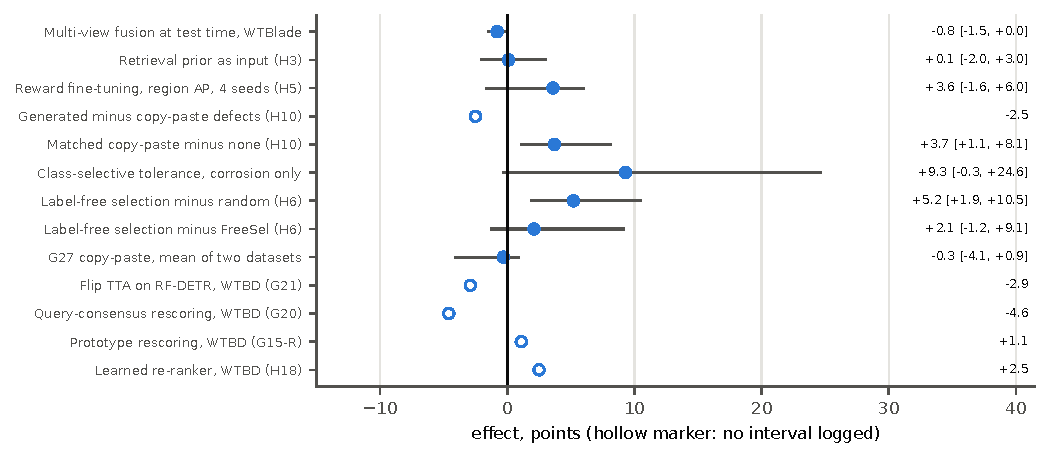
\includegraphics[width=\linewidth]{fig22_failed_tests}
\caption{Effects of method tests on leak-free test sets, in \mcoco points unless the ledger says otherwise; WTBD-group unless labelled. Hollow markers: no interval was logged in that form.}
\label{fig:failed}
\end{figure}

\begin{table*}[!t]
\centering
\caption{Ledger of method tests and diagnostics, in order of registration (H: hypothesis; G: gate). WTBD-group, test \mcoco points unless noted. Pre-registered from late October; earlier rounds were decided in advance but not formally committed.}
\label{tab:ledger}
\footnotesize
\begin{tabularx}{\textwidth}{@{}l X X l@{}}
\toprule
Test & Idea & Result & Verdict \\
\midrule
Phases 22--24 & Teacher--student with synthetic or real views, in-domain, class-balanced; 3 seeds & balanced in-domain 6.6 vs.\ supervised 7.9; \mfifty $-4.2$ \ci{-12.1}{-0.3}; runaway on one seed & fails \\
Phase 24 & SAM 2.1 box refinement~\cite{sam2} & $+0.3$ to $+0.5$ at 25\%, $-0.2$ at 100\% & fails \\
Phases 18, 26 & Split-tolerant training; class-selective version, 2 seeds & blanket not an improvement; corrosion $+9.3$ \ci{-0.3}{+24.6}, mean $-0.4$ & targeted only \\
H1 & Multi-view fusion at test time & untestable on WTBD (26 images with a second view); WTBlade-group $-0.8$ \ci{-1.5}{0.0} & fails \\
H2 & Normal-blade anomaly prior from DINOv3 patches & most anomalous patches not on defects; box recall below chance & fails \\
H3 & Retrieval prior (nearest labelled patches) as a detector input & $+0.1$ \ci{-2.0}{+3.0} & fails \\
H4 & Test-time adaptation across real views & gate failed: real views do not make better detections & not run \\
H5 & Reward fine-tuning with a granularity-invariant reward; 4 seeds + WTBlade & region AP $+3.6$ \ci{-1.6}{+6.0}, $P$ 0.896; WTBlade $-0.6$ & fails on replication \\
H6 & Label-free scene selection by patch coverage & $+5.2$ \ci{+1.9}{+10.5} over random; $+2.1$ \ci{-1.2}{+9.1} over FreeSel & no gain over prior art \\
H7 & Label-free property predicting subset quality & no property survives correction & fails \\
H8, H9 & Feature upsampling; high-frequency cues & $-5.9$; $-0.1$ & fail \\
H10 & Generated rare-class defects vs.\ matched copy-paste & synth $-$ paste $-2.5$; paste $-$ none $+3.7$ \ci{+1.1}{+8.1} & generation fails \\
H12 & DINOv3 reduces subset luck & it does not; draw quality carries over ($\rho$ 0.71) & fails \\
G15, G15-R & Prototype rescoring with DINOv3 box embeddings & WTBD $+1.1$; WTBlade $-0.7$ & fails bar; prior art \\
G16, G16-R & Instance-level proximity law; does it explain subset luck? & holds per instance; does not explain luck; on RF-DETR it governs confidence, not detection & partial \\
G17 & Clicks as pseudo-boxes (bar 60\% at IoU $\geq$0.5) & 42.0\% & fails \\
H18, -R, -W & Learned coverage-aware re-ranker on RF-DETR & WTBD $+2.5$, replicated on new models; WTBlade $+0.2$ & WTBD only \\
H19-W & Rescoring at the low-count boundary, WTBlade 8\% & $-0.2$ \ci{-1.3}{+0.7}, $P$ 0.286 & fails \\
G20 & Query-consensus rescoring & $-4.6$ WTBD; $-2.1$ WTBlade & fails \\
G21 & Flip agreement; plain flip TTA on RF-DETR & $-2.9$ WTBD; $-0.6$ WTBlade & fails; TTA hurts \\
G22, -O & Fine-tuning moves proximity from recall to ranking & confirmed on WTBD with a frozen-encoder control; not on WTBlade & does not replicate \\
H20 & Subset luck as annotation-convention match & no relation & fails \\
G24 & Input resolution 768 vs.\ 576 & WTBD $+1.0$ ($P$ 0.958); WTBlade $-0.1$ & dataset-specific \\
V1 & RF-DETR replaces the frozen-feature detector at 25\% & $+7.3$ \ci{+2.3}{+11.9}; $+8.3$ \ci{+4.5}{+15.0} & passes \\
G25, G26 & Official-protocol benchmark; tuned recipe & Tables~\ref{tab:official}, \ref{tab:tuning} & reported \\
G27 & CP, D1, D2 recipe & A-2 $-0.32$, $P$ 0.290 & fails \\
G28 & Leave-one-dataset-out & dead on both targets & fails \\
G29 & RF-DETR-FP, frozen DINOv3 prior & P $+1.45$, $P$ 0.958 (val $+0.20$); S $+1.38$, $P$ 0.856 & P passes narrowly; S fails \\
\bottomrule
\end{tabularx}
\end{table*}

\section{Discussion}
\label{sec:discussion}

\subsection{What the Benchmarks Measure}
On the official splits, a detector is largely asked to recognise images it has already seen in another orientation or exposure. The evidence is consistent across three independent measurements. The leaked and no-twin subsets differ by 24--48 \mfifty points on the two larger datasets. With the same model and recipe, swapping only the split halves \mcoco on WTBD. And a tuning step judged by the official numbers moved scores towards leaked images on all three datasets. The field's ``near-saturated'' 85--92 \mfifty therefore says little about inspection of new turbines. On leak-free splits the same detectors sit at 32--59 \mfifty and 13--35 \mcoco. That is the honest starting point for blade-defect detection on public data today.

\subsection{What Helps, and How Much}
Two things helped reliably: frozen foundation features in the YOLO family, and replacing the frozen-feature YOLO by a fine-tuned detection transformer at low label budgets (V1). Everything else we tried was either flat, dataset-specific or prior art. That covers semi-supervision, SAM refinement, split tolerance, reward fine-tuning, retrieval and anomaly priors, rescoring, flip agreement, resolution, copy-paste, encoder adaptation and pooled external data. RF-DETR-FP combines the two levers that worked. Its pre-registered test passes narrowly on test and is not confirmed on validation, so we report it as a small gain rather than a new state of the art. It does give the best leak-free WTBD result we have, and on the official protocol its change, unlike that of our tuning step, points towards unseen scenes.

\subsection{What Limits the Score}
Four ceilings stand out. (i) The annotators agree with themselves on only 84--87\% of labels on exact copies, and on 69\% for corrosion. (ii) Box granularity alone costs about 12 \apfifty points. (iii) Which 25\% of scenes are labelled changes the result by a factor of two. (iv) Detectors that see one site do not transfer to another, even from 35 times more images. At 25\% labels the dominant RF-DETR error is a correct box ranked low, not a missing box. On WTBlade, small cracks are missed at every budget.

\subsection{Recommendations}
\begin{enumerate}
\item \textbf{Split by scene, and deduplicate before augmenting.} Never augment before a split. Group by source photograph, video and tile, and add a pixel test: retrieval and keypoints alone missed photometric copies in our own splits.
\item \textbf{Publish image lists}, not just ratios. The question raised by BladeYOLO's 0.87 \mcoco/\mfifty ratio cannot be settled without one.
\item \textbf{Report a leaked/no-twin breakdown} for any dataset with known copies. It takes minutes with cached predictions, and our tools are public~\cite{repo}.
\item \textbf{Do not tune on a leaky test set.} On these splits, tuning measurably moved scores towards memorisation. Tune on a scene-separated validation set.
\item \textbf{Use scene-level intervals.} A 161-image test set with 58 scenes, some classes in fewer than three scenes, cannot support per-class claims.
\item \textbf{Report several labelled subsets for low-label claims.} A factor of two between random draws is larger than any model effect we saw.
\item \textbf{Report seeds and validation.} On these test sets, seed swings of up to 2 \mcoco points match the size of most claimed gains, and a test-only pass can fail to replicate.
\item \textbf{Calibrate on unseen scenes.} A recall guarantee calibrated on seen scenes does not hold in the field.
\item \textbf{Report a granularity-invariant score beside box AP} for amorphous defects, and measure label self-consistency where copies exist.
\item \textbf{Test every method on a second dataset.} Several of our effects held on WTBD and vanished on WTBlade, and the reverse.
\item \textbf{Check licences at the source}, since export pages can misstate them.
\end{enumerate}

\subsection{Limitations}
\label{sec:limits}
\begin{itemize}
\item \textbf{One wind farm per dataset, and small test sets} (58 and 177 test scenes), so our leak-free numbers carry wide intervals.
\item \textbf{Official-protocol runs are single seed}, and their intervals are image-level.
\item \textbf{The tuning analysis is post hoc and covers one step}, with epochs confounded on two of three protocols.
\item \textbf{Wind Surface's no-twin subset is not leak-free}, since it shares drone photographs with train. WTBD's no-twin subset has too few boxes of three classes.
\item \textbf{WTBlade-group frames retain Roboflow's offline augmentation.} We keep one copy per source, so some test frames are rotated or carry black cutouts (Fig.~\ref{fig:predictions}). This is a difference from clean imagery, not a leak.
\item \textbf{YOLO12-L on WTBlade-group may be under-trained:} 50 epochs, with its best validation at epoch 43 after a nearly linear rise.
\item \textbf{Our leak-free splits have a small residual leak}: under a point on WTBD-group, and negligible on WTBlade-group.
\item \textbf{RF-DETR-FP rests on two seeds} per leak-free dataset, and its gain is not confirmed on validation. WTBlade-Defect's official protocol was not run with the prior, as pre-registered: its 40-epoch twin would not fit a 12\,h T4 session.
\item \textbf{G27 A-2 uses two seeds, and G28 one.} G28's X arms train for 12 epochs at 640\,px, and X-WTBlade's pool is 45\% smaller than X-WTBD's.
\item \textbf{Hardware differs between some seeds} (T4 fp16 and A100 bf16). Arms are always paired within a hardware type.
\item \textbf{Claims about modules concern our components.} BladeYOLO's own modules were not rerun on a leak-free split after the code audit.
\item \textbf{Deviations from pre-registration.} The G26 rule formally selected RF-DETR-L (validation 63.4 against 62.0), which lost on test ($-1.7$), and we did not run L on the other protocols; this cannot inflate a reported number. G27's phase B on the official protocols was not run, since the recipe failed A-2.
\item \textbf{The literature check is not exhaustive}; ``new for this domain'' means that we did not find an earlier audit.
\end{itemize}

\section{Conclusion}
The three public blade-defect benchmarks mostly test memorisation: 78--92\% of their official test images have a training twin, and their published 85--92 \mfifty fall to 32--59 on scene-grouped splits of the same images. Our attempt to reproduce BladeYOLO taught us this the hard way, through a 52.6 faithful reimplementation, a 78.2 that was itself leaked and a code audit that invalidated our own early conclusions. We release audited leak-free splits of WTBD and WTBlade-Defect with scene-level intervals, per-image leak flags for the official test sets and all evaluation tools. On these benchmarks, frozen foundation features are the one ingredient that reliably helps a YOLO detector. A fine-tuned detection transformer is stronger still at low labels on WTBD. Our RF-DETR-FP, which keeps a frozen DINOv3 prior beside RF-DETR's fine-tuned encoder, gives the best WTBD-group result (34.4 \mcoco) in a narrow, pre-registered pass. The larger lesson is about measurement. Without scene-level splits, leak breakdowns, seeds and pre-registration, every number in this field, including several of our own, would have pointed in the wrong direction.

\section*{Data and Code Availability}
\textbf{Code and records.} All code, tests, split files, per-image leak flags, cached predictions and the full research log (\texttt{research\_log.md}) are at \url{https://github.com/bhavya-goel-11/BladeYOLO}~\cite{repo}. To regenerate this paper's numbers and figures, run \texttt{tools/official\_leak\_eval.py}, \texttt{tools/g27\_score.py}, \texttt{tools/g28\_score.py}, \texttt{tools/g29\_score.py}, \texttt{tools/paper\_evidence.py}, \texttt{tools/paper\_figures.py}, \texttt{tools/paper\_figures2.py}, \texttt{tools/paper\_figures3.py} and \texttt{tools/build\_ieee\_tables.py}. The training queue is \texttt{tools/sessions.sh}. RF-DETR-FP is \texttt{tools/g29\_prior.py}, with unit and end-to-end tests in \texttt{tests/test\_g29\_prior.py}.

\textbf{Data.} The datasets as audited, the leak-free splits (WTBD-group, WTBlade-group), the official splits used here and the twin-free pools are assembled as \texttt{blade-defect-benchmark} on Kaggle: \url{https://www.kaggle.com/datasets/beegee11/blade-defect-benchmark}~\cite{kaggleds}. Per-folder licences are in its \texttt{LICENSES.md}. WTBD is CC BY 4.0~\cite{wtbd}. WTBlade-Defect contains DTU NordTank images~\cite{shihavuddin,dtudata} under CC BY-NC, despite its Roboflow page, and derived folders inherit this, so they are for non-commercial research only. The Wind Surface licence is unclear from its source~\cite{gfdyolox}. Images in our figures are shown for scientific comment, and their sources are cited.

\textbf{Foundation models.} We acknowledge DINOv3~\cite{dinov3}, used under the DINOv3 License, and DINOv2~\cite{dinov2} through RF-DETR~\cite{rfdetr} (Apache-2.0). Trained checkpoints that contain DINOv3 weights must ship with that licence; RF-DETR-FP checkpoints contain only the fusion layers.


% main-text floats are flushed before the appendices; appendices (one column), acknowledgment and references close the paper
\clearpage
\appendices
\onecolumn
\setlength{\LTpre}{4pt}\setlength{\LTpost}{4pt}
\LTchunksize=200
\section{Project Timeline}
\label{app:timeline}
Table~\ref{tab:timeline} lists the phases of the project as recorded in the research log, so that every result in this paper can be placed in its context.

\begin{table*}[!htbp]
\centering
\caption{Project timeline (2026). Section numbers refer to the research log~\cite{repo}.}
\label{tab:timeline}
\footnotesize
\begin{tabularx}{\textwidth}{@{}l l X@{}}
\toprule
Dates & Phase & Content and outcome \\
\midrule
3 Sep -- 6 Oct & 1--5 & Faithful BladeYOLO reimplementation (Runs 1--3, best 52.6/28.0); BladeYOLO-S and -L (64.3/37.3; 78.2/46.9 on the leaky split) \\
9 Oct & 6 & Code audit: WIoU inactive, no selective scan, DINOv3 without RoPE or normalisation, wavelet detail lost; all repaired and tested \\
9 Oct & 7 & Wind Surface leak found: 75\% of validation images have a pixel twin; tiles of 386 photographs on both sides \\
9--12 Oct & 8--12 & Merged, deduplicated datasets v2 (2{,}606 images) and v3 (5{,}777); 26--40 \mfifty; label review worth $+3$; BladeYOLO-v2 designed; NaN root causes fixed; ceiling about 40--45 \mfifty on v3 \\
12--13 Oct & 13 & Content audit of six datasets; WTBD chosen; WTBD-group split built and audited \\
13--14 Oct & 14--15 & Same model on official vs.\ group WTBD split: $+29$ \mfifty inflation; YOLO12-L baselines; scene bootstrap \\
14--15 Oct & 16--18 & Granularity-aware scores; cross-view label audit (84--87\% agreement); conformal recall failure under leaked calibration; split-tolerant training; YOLOv12 area attention fp16 overflow fixed \\
15--18 Oct & 19--24 & Real-view teacher--student semi-supervision (three rounds, dropped); SAM 2.1 refinement (fails) \\
18--21 Oct & 25--27 & DINOv3 ablation across 25/50/100\%; class-selective tolerance; backbone size (ViT-B best) \\
21 Oct -- 2 Nov & 28--31 & Pre-registered hypotheses H1--H20 and gates G8--G24 on WTBD-group and WTBlade-group (Table~\ref{tab:ledger}); V1: RF-DETR at low labels passes \\
2--4 Nov & G25, G26 & RF-DETR on the official protocols; tuned recipe; leaked vs.\ no-twin analysis; tuning rewards memorisation \\
4--8 Nov & G27, G28 & One recipe for all protocols (copy-paste, encoder SSL, multi-dataset stage 1): fails. Leave-one-dataset-out: dead \\
8 Nov & -- & First paper draft; residual pixel twins found in our own splits \\
16--17 Nov & G29 & RF-DETR-FP pre-registered, run on two Kaggle sessions (four T4 lanes), scored: primary passes narrowly, secondary fails \\
\bottomrule
\end{tabularx}
\end{table*}

\section{Corrections to Our Own Conclusions}
\label{app:corrections}
Table~\ref{tab:corrections} lists the conclusions we later corrected. Several were our own favourite explanations.

\begin{table*}[!htbp]
\centering
\caption{Conclusions we later corrected. Kept because each was plausible at the time.}
\label{tab:corrections}
\footnotesize
\begin{tabularx}{\textwidth}{@{}X l X@{}}
\toprule
Earlier conclusion & Status & Why \\
\midrule
Runs 6--7 reach $\sim$78/$\sim$47 on Wind Surface & invalid & 75\% of validation had train twins (first count) \\
WIoU v3 gave $+0.9$ \mcoco & invalid & never active; Run 7 trained with CIoU \\
Mamba added global context & invalid & the block did not scan \\
SGD $\rightarrow$ AdamW was the breakthrough & confounded & changed together with an 8\,M $\rightarrow$ 57\,M scale-up \\
The remaining gap is locality bias & superseded & the gap was leakage and data structure \\
v3 is better because it is larger & superseded & scenes matter, not files (Wind Surface 81 scenes; WTBD 550) \\
Mislabelling explains poor v3 scores & rejected & the review was worth only $+3$ \mfifty \\
BladeYOLO-v2's win shows the architecture generalises & qualified & it rests mainly on thunderstrike (3 test scenes) \\
The advantage comes from the architecture & rejected & the frozen DINOv3 features carry it all \\
Honest calibration costs 2.4 vs.\ 1.0 false alarms per image & corrected & that column counted all predictions; real false alarms 0.2 vs.\ 0.1 \\
WTBD copies agree on 86.0\% & refined & rotated copies inflate ``loose''; axis-aligned 87.3\% \\
Part of the inflation is memorised box splitting & not supported & tolerant gain is not smaller on images with a twin \\
At 25\%, most lost defects are found but boxed differently & refined & near-misses (34--36\%) and misses (19--27\%) are of similar size \\
Split tolerance helps corrosion & replicated, not significant & $+9.3$ \ci{-0.3}{+24.6}; aggregate unchanged \\
The DINOv3 advantage is a low-data advantage & corrected & absolute gain does not shrink with data \\
The gain grows with frozen backbone size & partly supported & ViT-B beats ViT-S; ViT-L does not beat ViT-B \\
Teacher--student gives a small consistent gain & qualified & seed noise was as large; balanced variant significantly worse \\
Leak-free \mcoco/\mfifty ratios are 0.42--0.47 & corrected & full-label RF-DETR on WTBD-group reaches 0.60 \\
Our leak-free splits are twin-free & corrected & a pixel test found 6+6 WTBD-group and 1+1 WTBlade-group copies; effect under one point \\
A frozen prior helps RF-DETR most on WTBlade and on rare classes (G29 prediction) & not supported & gain larger on WTBD, in frequent classes \\
\bottomrule
\end{tabularx}
\end{table*}

\section{Engineering Problems That Affected Results}
\label{app:engineering}
Table~\ref{tab:engineering} lists defects we found and fixed. Several silently changed what was being measured; mixed-precision overflow was the most frequent.

\begin{table*}[!htbp]
\centering
\caption{Engineering defects found and fixed.}
\label{tab:engineering}
\footnotesize
\begin{tabularx}{\textwidth}{@{}X X X@{}}
\toprule
Problem & Root cause & Fix \\
\midrule
WIoU never active & patched the wrong namespace & patch the loss namespace \\
NaN in selective scan (epoch 9) & fp16 overflow before LayerNorm & fp32 LayerNorm \\
NaN at epoch 4 & poisoned WIoU running mean; aggressive warm-up & finite-only mean; lr 0.001, bias warm-up 0 \\
NaN at epoch 17 & fp16 overflow from a convolution into BatchNorm & fp32 blocks for refinement \\
NaN at epoch 99, validation at 0 & a NaN batch poisons BatchNorm statistics and EMA & per-batch BatchNorm repair and step skip, reported \\
NaN late in training (epochs 99--149) & YOLOv12 area attention forms scores in fp16 ($\sim$4e5, above the fp16 maximum) & scores and softmax in fp32 \\
Test metrics silently missing & \texttt{deform\_conv2d} segfault on NaN offsets from the FLOPs probe's uninitialised image & finite, clamped offsets; test in a fresh process \\
Silent resume from an old checkpoint & training script reused any \texttt{last.pt} & explicit \texttt{--resume} \\
RF-DETR learning rate never decayed & default step at epoch 100 never fires & explicit cosine schedule (G26) \\
Scorer read a stale result after a time-out & an earlier output file had the same name & rerun with no limit; check file freshness \\
Official-protocol tool returned empty WTBlade subsets & split parsed from a path component that moved in a data migration & split taken from the folder above \texttt{images/}; earlier rows reproduce exactly \\
Kaggle sessions cut at 12\,h & two runs per session, one per T4 & time guard: no start with $<$30\,min left, SIGINT 15\,min before the budget, stopped runs renamed and never scored \\
\bottomrule
\end{tabularx}
\end{table*}

\section{Notation and Experiment Names}
Names follow the research log: H$n$ and G$n$ are hypotheses and gates in order of registration. A0--A3 are the G27 arms: A0 plain recipe, A1 + copy-paste, A2 + copy-paste + D1, A3 + copy-paste + D2. FP is RF-DETR-FP (G29). ID and X are the G28 arms. V1 is the 25\% RF-DETR comparison. ``Points'' are percentage points of AP. WTBD-official is WTBD's own split. BYv2 is BladeYOLO-v2.

\section{Per-Class Audit and Run Registry}
\label{app:registry}
Table~\ref{tab:perclass-audit} gives the content audit by native class for every dataset we audited. Table~\ref{tab:newruns} lists every run of the final phase with its validation and test scores, and Table~\ref{tab:registry} the registry of all earlier runs as kept in the research log.
% generated by tools/build_ieee_tables.py; do not edit
\begin{longtable}{@{}l l r r r r r r r@{}}
\caption{Content audit by native class (\texttt{runs/analysis/datasets/report.md}). \emph{Learnable} boxes are those kept after deduplication. \emph{Purity} is mutual crop retrieval within the class. Median box size is in pixels at 640. The check export of Beijing is omitted because it is the same data.}\label{tab:perclass-audit}\\
\toprule
Dataset & Class & Raw img & Raw boxes & Unique & Scenes & Learnable & Median px & Purity \\
\midrule
\endfirsthead
\toprule Dataset & Class & Raw img & Raw boxes & Unique & Scenes & Learnable & Median px & Purity \\\midrule
\endhead
Wind Surface & corrosion & 660 & 2116 & 90 & 10 & 294 & 87.7 & 0.894 \\
Wind Surface & dirt & 1044 & 1067 & 487 & 14 & 488 & 257.3 & 0.923 \\
Wind Surface & hide\_craze & 1305 & 2321 & 272 & 50 & 491 & 53.6 & 0.719 \\
Wind Surface & surface\_eye & 108 & 412 & 9 & 1 & 40 & 85.5 & 0.0 \\
Wind Surface & thunderstrike & 364 & 478 & 70 & 10 & 89 & 55.5 & 0.12 \\
WTBlade & burn & 736 & 1019 & 116 & 104 & 166 & 56.9 & 0.65 \\
WTBlade & crack & 1409 & 2525 & 177 & 112 & 335 & 63.0 & 0.573 \\
WTBlade & deformity & 1801 & 2291 & 282 & 231 & 383 & 130.7 & 0.802 \\
WTBlade & dirt & 5148 & 8875 & 585 & 425 & 928 & 255.2 & 0.683 \\
WTBlade & oil & 539 & 958 & 97 & 82 & 167 & 105.6 & 0.428 \\
WTBlade & peeling & 2307 & 5715 & 172 & 80 & 395 & 96.5 & 0.583 \\
WTBlade & rust & 2043 & 4188 & 157 & 123 & 258 & 95.2 & 0.354 \\
Beijing & corrosion & 789 & 2565 & 90 & 10 & 292 & 86.9 & 0.666 \\
Beijing & craze & 57 & 69 & 9 & 8 & 12 & 158.3 & 0.108 \\
Beijing & hide\_craze & 1187 & 2137 & 283 & 52 & 499 & 54.9 & 0.545 \\
Beijing & surface\_eye & 3316 & 5489 & 900 & 17 & 1467 & 227.3 & 0.888 \\
Beijing & surface\_injure & 1662 & 3285 & 290 & 45 & 564 & 85.3 & 0.635 \\
Beijing & surface\_oil & 1588 & 2242 & 417 & 27 & 574 & 249.9 & 0.473 \\
Beijing & thunderstrike & 270 & 353 & 69 & 10 & 87 & 52.2 & 0.153 \\
WTBs2025 & oil leakage & 512 & 572 & 28 & 28 & 35 & 33.9 & 0.486 \\
WTBs2025 & paint cracks & 458 & 514 & 398 & 351 & 235 & 17.8 & 0.666 \\
WTBs2025 & localized damage & 1027 & 1254 & 773 & 655 & 86 & 6.5 & 0.256 \\
WTBs2025 & lightning strikes & 285 & 354 & 89 & 43 & 96 & 43.1 & 0.56 \\
WTBs2025 & surface stains & 263 & 294 & 226 & 211 & 142 & 23.5 & 0.182 \\
WTBs2025 & erosion & 2798 & 4517 & 1132 & 993 & 1174 & 21.4 & 0.675 \\
WTBs2025 & coating detachment & 1085 & 1906 & 703 & 566 & 526 & 15.3 & 0.484 \\
WTBs2025 & protective film damage & 546 & 632 & 393 & 350 & 195 & 14.2 & 0.639 \\
WTBs2025 & pinholes & 522 & 774 & 377 & 311 & 45 & 2.2 & 0.136 \\
WTBD & craze & 198 & 257 & 94 & 86 & 119 & 206.5 & 0.555 \\
WTBD & corrosion & 172 & 257 & 105 & 100 & 149 & 194.3 & 0.723 \\
WTBD & surface\_injure & 264 & 412 & 164 & 155 & 247 & 103.3 & 0.723 \\
WTBD & thunderstrike & 89 & 92 & 50 & 47 & 52 & 138.0 & 0.565 \\
WTBD & crack & 177 & 224 & 47 & 37 & 55 & 171.5 & 0.842 \\
WTBD & hide\_craze & 249 & 342 & 182 & 171 & 244 & 111.9 & 0.785 \\
\bottomrule
\end{longtable}

% generated by tools/build_ieee_tables.py; do not edit
{\scriptsize
\begin{longtable}{@{}l l l l l@{}}
\caption{Runs of the final phase (G26--G29, G28, YOLO12-L). Val best is the best EMA epoch on validation (Ultralytics' best epoch for YOLO12-L), with the epoch in parentheses; test values are those of the tables in the main text (COCO-style evaluator, percent). On the 25\% runs only \mcoco was scored per subset.}\label{tab:newruns}\\
\toprule
Run & Data, arm & Epochs (best) & Val best \mfifty / \mcoco & Test \mfifty / \mcoco \\
\midrule
\endfirsthead
\toprule Run & Data, arm & Epochs (best) & Val best & Test \\\midrule
\endhead
\texttt{rfdetrm768cos\_wtbd\_group\_full} & WTBD-group, A0, s0 & 100 (20) & 64.8 / 40.4 & 55.3 / 33.2 \\
\texttt{rfdetrm768cos\_wtbd\_group\_full\_s1} & WTBD-group, A0, s1 (T4) & 100 (31) & 66.6 / 40.1 & 53.2 / 31.2 \\
\texttt{rfdetrm768cos\_wtbd\_group\_full\_s1} & WTBD-group, A0, s1 (A100) & 100 (32) & 67.1 / 40.8 & 54.8 / 32.2 \\
\texttt{rfdetrm768cos\_cp\_wtbd\_group\_full} & WTBD-group, A1, s0 & 100 (9) & 63.9 / 40.1 & 51.5 / 30.7 \\
\texttt{rfdetrm768cos\_cp\_wtbd\_group\_full\_s1} & WTBD-group, A1, s1 & 100 (31) & 70.7 / 41.8 & 58.5 / 32.7 \\
\texttt{rfdetrm768cos\_cp\_d1\_wtbd\_group\_full} & WTBD-group, A2 & 100 (63) & 59.6 / 34.4 & 49.6 / 27.4 \\
\texttt{rfdetrm768cos\_cp\_d2\_wtbd\_group\_full} & WTBD-group, A3 & 100 (40) & 56.8 / 33.8 & 55.3 / 33.2 \\
\texttt{rfdetrm768cos\_fp\_wtbd\_group\_full} & WTBD-group, FP, s0 & 100 (33) & 70.7 / 42.0 & 58.7 / 34.3 \\
\texttt{rfdetrm768cos\_fp\_wtbd\_group\_full\_s1} & WTBD-group, FP, s1 & 100 (100) & 67.3 / 39.4 & 59.1 / 34.5 \\
\texttt{rfdetrm640cos\_wtblade\_group\_full} & WTBlade-group, A0, s0 & 60 (11) & 38.4 / 15.7 & 38.5 / 16.2 \\
\texttt{rfdetrm640cos\_wtblade\_group\_full\_s1} & WTBlade-group, A0, s1 (T4) & 60 (15) & 41.0 / 16.6 & 41.5 / 16.9 \\
\texttt{rfdetrm640cos\_wtblade\_group\_full\_s1} & WTBlade-group, A0, s1 (A100) & 60 (17) & 41.1 / 16.2 & 41.0 / 16.9 \\
\texttt{rfdetrm640cos\_cp\_wtblade\_group\_full} & WTBlade-group, A1, s0 & 60 (13) & 41.6 / 17.1 & 41.8 / 17.3 \\
\texttt{rfdetrm640cos\_cp\_wtblade\_group\_full\_s1} & WTBlade-group, A1, s1 & 60 (16) & 41.3 / 16.9 & 39.3 / 16.5 \\
\texttt{rfdetrm640cos\_cp\_d1\_wtblade\_group\_full} & WTBlade-group, A2 & 60 (16) & 39.2 / 15.7 & 40.1 / 16.1 \\
\texttt{rfdetrm640cos\_cp\_d2\_wtblade\_group\_full} & WTBlade-group, A3 & 60 (8) & 44.2 / 17.8 & 41.7 / 16.6 \\
\texttt{rfdetrm640cos\_fp\_wtblade\_group\_full} & WTBlade-group, FP, s0 & 60 (13) & 40.6 / 16.1 & 41.6 / 17.3 \\
\texttt{rfdetrm640cos\_fp\_wtblade\_group\_full\_s1} & WTBlade-group, FP, s1 & 60 (13) & 41.1 / 16.1 & 40.5 / 17.2 \\
\texttt{rfdetrm768cos\_wtbd\_official} & WTBD-official, G26 & 100 (49) & 92.5 / 62.0 & 90.4 / 61.2 \\
\texttt{rfdetrm768cos\_fp\_wtbd\_official} & WTBD-official, FP & 100 (78) & 89.3 / 61.5 & 90.9 / 59.9 \\
\texttt{rfdetrm640cos\_windsurface\_official} & Wind Surface, G26 & 100 (94) & 82.1 / 54.4 & 81.0 / 53.3 \\
\texttt{rfdetrm640cos\_fp\_windsurface\_official} & Wind Surface, FP & 100 (60) & 83.1 / 53.0 & 82.1 / 51.7 \\
\texttt{rfdetrm640cos\_wtblade\_defect\_official} & WTBlade-Defect, G26 & 40 (40) & 89.4 / 55.7 & 87.2 / 55.1 \\
\texttt{rfdetrmfp\_wtbd\_group\_f25} & WTBD-group 25\%, class-matched, FP & 100 (58) & 45.1 / 26.5 & -- / 24.6 \\
\texttt{rfdetrmfp\_rand1\_wtbd\_group\_f25} & WTBD-group 25\%, rand1, FP & 100 (69) & 49.5 / 30.0 & -- / 20.4 \\
\texttt{rfdetrmfp\_rand2\_wtbd\_group\_f25} & WTBD-group 25\%, rand2, FP & 100 (70) & 45.7 / 28.8 & -- / 22.1 \\
\texttt{rfdetrmfp\_rand3\_wtbd\_group\_f25} & WTBD-group 25\%, rand3, FP & 100 (15) & 39.2 / 23.7 & -- / 14.1 \\
\texttt{rfdetrm640ag\_id\_wtbd\_group} & ID-WTBD, class-agnostic & 100 (23) & 80.7 / 48.3 & 72.9 / 41.9 \\
\texttt{rfdetrm640ag\_id\_wtblade\_group} & ID-WTBlade, class-agnostic & 60 (26) & 49.5 / 20.5 & 51.7 / 21.5 \\
\texttt{rfdetrm640ag\_x\_wtbd\_group} & X-WTBD, class-agnostic (own val) & 12 (12) & 72.2 / 38.6 & 17.7 / 6.0 \\
\texttt{rfdetrm640ag\_x\_wtblade\_group} & X-WTBlade, class-agnostic (own val) & 12 (12) & 62.1 / 33.6 & 2.4 / 0.5 \\
\texttt{yolo12l\_wtblade\_group} & WTBlade-group, YOLO12-L & 50 (43) & 33.6 / 12.5 & 32.2 / 13.3 \\
\bottomrule
\end{longtable}
}

% generated by tools/build_ieee_tables.py; do not edit
{\scriptsize
\setlength{\tabcolsep}{3pt}
\begin{longtable}{@{}p{0.2\textwidth} p{0.12\textwidth} p{0.15\textwidth} p{0.06\textwidth} p{0.1\textwidth} p{0.13\textwidth} p{0.12\textwidth}@{}}
\caption{Registry of the runs before the final phase, as kept in the research log (section 27 there; section references inside this table are to the log). Scores are fractions, not percent. WS: Wind Surface.}\label{tab:registry}\\
\toprule
Run folder & Data & Model & Epochs & Val best (50 / 50:95) & Test (50 / 50:95) & Notes \\
\midrule
\endfirsthead
\toprule Run folder & Data & Model & Epochs & Val best & Test & Notes \\\midrule
\endhead
Runs 1--5 & WS original & Paper-faithful / BladeYOLO-S & -- & see \S2 & -- & Logs on Kaggle only \\
\texttt{bladeyolo\_\allowbreak l\_\allowbreak sota} (Run 6) & WS original (\textbf{leaky}) & BladeYOLO-L & 400 & 0.781 / 0.469 & -- & Inflated \\
\texttt{bladeyolo\_\allowbreak l\_\allowbreak sota-2} (Run 7) & WS original (\textbf{leaky}) & BladeYOLO-L + "Mamba" + (inactive) WIoU & 400 & 0.769 / 0.478 & -- & Inflated \\
\texttt{yolo12l\_\allowbreak baseline} & v2 & YOLO12-L & 266 & 0.290 / 0.122 & 0.358 / 0.149 & lr0 0.002 \\
\texttt{bladeyolo\_\allowbreak l} & v2 & BladeYOLO-L (repaired) & 167 (stopped) & 0.344 / 0.123 & 0.400 / 0.146 (epoch 124) &  \\
\texttt{yolo12l\_\allowbreak v3} & v3 & YOLO12-L & 150 & 0.290 / 0.141 & 0.263 / 0.109 & Old harmful recipe \\
\texttt{bladeyolo\_\allowbreak v3} & v3 & BladeYOLO-L v1 & 150 & 0.356 / 0.156 & 0.317 / 0.124 &  \\
\texttt{bladeyolo2\_\allowbreak v3} & v3 & BladeYOLO-v2 & 100 & 0.369 / 0.172 & 0.296 / 0.123 (evaluator) & Test lost on Kaggle (segfault) \\
WBF ensemble & v3 / v3.2 & 3 models & -- & -- & 0.339 / 0.143 (v3); $\sim$0.411 / 0.168 (merged) & Fusion IoU chosen on val \\
\texttt{bladeyolo2\_\allowbreak wtbd\_\allowbreak group} (attempt 1) & WTBD-group & BladeYOLO-v2 & 99 of 150 & 0.649 / 0.379 & -- & NaN at epoch 99; folder lost \\
\textbf{\texttt{bladeyolo2\_\allowbreak wtbd\_\allowbreak group}} & WTBD-group (leak-free) & BladeYOLO-v2 & 150 & 0.650 / 0.368 (epoch 124) & \textbf{0.548 / 0.245}; TTA 0.574 / 0.279 & Test run locally \\
\textbf{\texttt{bladeyolo2\_\allowbreak wtbd\_\allowbreak official}} & WTBD official (\textbf{leaky}) & BladeYOLO-v2 & 120 & 0.845 / 0.475 (epoch 105) & \textbf{0.840 / 0.493}; TTA 0.830 / 0.517 & TTA run locally \\
\textbf{\texttt{bladeyolo2\_\allowbreak wtbd\_\allowbreak group\_\allowbreak tolerant}} & WTBD-group (leak-free) & BladeYOLO-v2, split-tolerant targets & 150 & 0.609 / 0.352 (epoch 83) & \textbf{0.523 / 0.249}; TTA 0.552 / 0.282 & 5 NaN batches dropped (attention overflow, since fixed) \\
\texttt{bladeyolo2\_\allowbreak wtbd\_\allowbreak group\_\allowbreak f25} & WTBD-group, 25\% of train scenes & BladeYOLO-v2 & 150 & 0.444 / 0.226 (epoch 126) & \textbf{0.232 / 0.082}; TTA 0.269 / 0.105 & Learning curve \\
\texttt{bladeyolo2\_\allowbreak wtbd\_\allowbreak group\_\allowbreak f50} & WTBD-group, 50\% of train scenes & BladeYOLO-v2 & 150 & 0.472 / 0.263 (epoch 140) & \textbf{0.413 / 0.183}; TTA 0.473 / 0.211 & Learning curve \\
\texttt{yolo12l\_\allowbreak wtbd\_\allowbreak group\_\allowbreak f25} & WTBD-group, 25\% of train scenes & YOLO12-L & 150 & 0.233 / 0.139 (epoch 150) & \textbf{0.106 / 0.037}; TTA 0.144 / 0.059 & Learning curve \\
\texttt{yolo12l\_\allowbreak wtbd\_\allowbreak group\_\allowbreak f50} & WTBD-group, 50\% of train scenes & YOLO12-L & 150 & 0.279 / 0.167 (epoch 120) & \textbf{0.244 / 0.105}; TTA 0.259 / 0.125 & Learning curve \\
\texttt{bladeyolo2\_\allowbreak wtbd\_\allowbreak group\_\allowbreak f25\_\allowbreak sslsyn} & WTBD-group 25\% + view pool & BladeYOLO-v2, synthetic-view teacher--student & 150 & 0.427 / 0.203 (epoch 142) & \textbf{0.221 / 0.071}; TTA 0.233 / 0.089 & Phase 22 \\
\texttt{bladeyolo2\_\allowbreak wtbd\_\allowbreak group\_\allowbreak f25\_\allowbreak sslreal} & WTBD-group 25\% + view pool & BladeYOLO-v2, real-view teacher--student & 150 & 0.450 / 0.210 (epoch 107) & \textbf{0.213 / 0.085}; TTA 0.268 / 0.107 & Phase 22; teacher collapsed \\
\texttt{bladeyolo2\_\allowbreak wtbd\_\allowbreak group\_\allowbreak f25\_\allowbreak sslsyn2} & WTBD-group 25\% + view pool & BladeYOLO-v2, synthetic views (fixed) & 150 & 0.448 / 0.220 (epoch 122) & \textbf{0.224 / 0.078}; TTA 0.259 / 0.106 & Phase 23 \\
\texttt{bladeyolo2\_\allowbreak wtbd\_\allowbreak group\_\allowbreak f25\_\allowbreak sslreal2} & WTBD-group 25\% + view pool & BladeYOLO-v2, real views (fixed) & 150 & 0.382 / 0.184 (epoch 127) & \textbf{0.192 / 0.077}; TTA 0.248 / 0.101 & Phase 23 \\
\texttt{bladeyolo2\_\allowbreak wtbd\_\allowbreak group\_\allowbreak f25\_\allowbreak sslin} & WTBD-group 25\% + other 75\% unlabelled & BladeYOLO-v2, in-domain teacher--student & 150 & 0.457 / 0.227 (epoch 131) & \textbf{0.209 / 0.080}; TTA 0.245 / 0.101 & Phase 23 \\
\texttt{bladeyolo2\_\allowbreak wtbd\_\allowbreak group\_\allowbreak f25\_\allowbreak s1} & WTBD-group, 25\% of train scenes & BladeYOLO-v2, seed 1 & 150 & 0.411 / 0.199 (epoch 129) & \textbf{0.224 / 0.087}; TTA 0.242 / 0.105 & Phase 24 \\
\texttt{bladeyolo2\_\allowbreak wtbd\_\allowbreak group\_\allowbreak f25\_\allowbreak s2} & WTBD-group, 25\% of train scenes & BladeYOLO-v2, seed 2 & 150 & 0.435 / 0.203 (epoch 143) & \textbf{0.184 / 0.068}; TTA 0.229 / 0.096 & Phase 24 \\
\texttt{bladeyolo2\_\allowbreak wtbd\_\allowbreak group\_\allowbreak f25\_\allowbreak sslinb\_\allowbreak s0} & WTBD-group 25\% + other 75\% unlabelled & BladeYOLO-v2, in-domain, class-balanced, seed 0 & 150 & 0.344 / 0.154 (epoch 75) & \textbf{0.143 / 0.060}; TTA 0.183 / 0.079 & Phase 24 \\
\texttt{bladeyolo2\_\allowbreak wtbd\_\allowbreak group\_\allowbreak f25\_\allowbreak sslinb\_\allowbreak s1} & WTBD-group 25\% + other 75\% unlabelled & same, seed 1 & 150 & 0.352 / 0.167 (epoch 92) & \textbf{0.163 / 0.065}; TTA 0.180 / 0.075 & Phase 24; pseudo-label runaway, epochs 33--62 \\
\texttt{bladeyolo2\_\allowbreak wtbd\_\allowbreak group\_\allowbreak f25\_\allowbreak sslinb\_\allowbreak s2} & WTBD-group 25\% + other 75\% unlabelled & same, seed 2 & 150 & 0.445 / 0.205 (epoch 148) & \textbf{0.183 / 0.073}; TTA 0.213 / 0.095 & Phase 24 \\
\texttt{bladeyolo2nodino\_\allowbreak wtbd\_\allowbreak group\_\allowbreak f25\_\allowbreak s0} & WTBD-group, 25\% of train scenes & BladeYOLO-v2 without DINOv3, seed 0 & 150 & 0.229 / 0.126 (epoch 106) & \textbf{0.114 / 0.044}; TTA 0.153 / 0.063 & Phase 25 \\
\texttt{bladeyolo2nodino\_\allowbreak wtbd\_\allowbreak group\_\allowbreak f25\_\allowbreak s1} & WTBD-group, 25\% of train scenes & BladeYOLO-v2 without DINOv3, seed 1 & 150 & 0.186 / 0.105 (epoch 89) & \textbf{0.081 / 0.031}; TTA 0.126 / 0.053 & Phase 25 \\
\texttt{bladeyolo2\_\allowbreak wtbd\_\allowbreak group\_\allowbreak s1} & WTBD-group (leak-free) & BladeYOLO-v2, seed 1 & 150 & 0.630 / 0.370 (epoch 128) & \textbf{0.554 / 0.245}; TTA 0.559 / 0.269 & Phase 26; resumed at epoch 78 \\
\texttt{bladeyolo2\_\allowbreak wtbd\_\allowbreak group\_\allowbreak tolsel\_\allowbreak s0} & WTBD-group (leak-free) & BladeYOLO-v2, tolerance for corrosion + hide\_craze, seed 0 & 150 & 0.656 / 0.381 (epoch 140) & \textbf{0.567 / 0.245}; TTA 0.568 / 0.258 & Phase 26 \\
\texttt{bladeyolo2\_\allowbreak wtbd\_\allowbreak group\_\allowbreak tolsel\_\allowbreak s1} & WTBD-group (leak-free) & same, seed 1 & 150 & 0.704 / 0.380 (epoch 119) & \textbf{0.561 / 0.245}; TTA 0.555 / 0.264 & Phase 26 \\
\texttt{bladeyolo2b\_\allowbreak wtbd\_\allowbreak group\_\allowbreak f25\_\allowbreak s0} & WTBD-group, 25\% of train scenes & BladeYOLO-v2, frozen DINOv3 ViT-B/16, seed 0 & 150 & 0.383 / 0.176 (epoch 127) & \textbf{0.252 / 0.102}; TTA 0.313 / 0.127 & Phase 27 \\
\texttt{bladeyolo2b\_\allowbreak wtbd\_\allowbreak group\_\allowbreak f25\_\allowbreak s1} & WTBD-group, 25\% of train scenes & same, seed 1 & 150 & 0.416 / 0.217 (epoch 146) & \textbf{0.283 / 0.116}; TTA 0.272 / 0.132 & Phase 27 \\
\texttt{bladeyolo2l\_\allowbreak wtbd\_\allowbreak group\_\allowbreak f25\_\allowbreak s0} & WTBD-group, 25\% of train scenes & BladeYOLO-v2, frozen DINOv3 ViT-L/16, seed 0 & 150 & 0.438 / 0.219 (epoch 107) & \textbf{0.337 / 0.115}; TTA 0.357 / 0.153 & Phase 27 \\
\texttt{bladeyolo2l\_\allowbreak wtbd\_\allowbreak group\_\allowbreak f25\_\allowbreak s1} & WTBD-group, 25\% of train scenes & same, seed 1 & 150 & 0.484 / 0.235 (epoch 81) & \textbf{0.301 / 0.109}; TTA 0.348 / 0.146 & Phase 27 \\
\texttt{bladeyolo2nodino\_\allowbreak wtbd\_\allowbreak group\_\allowbreak f50} & WTBD-group, 50\% of train scenes & BladeYOLO-v2 without DINOv3 & 150 & 0.293 / 0.166 (epoch 105) & \textbf{0.225 / 0.093}; TTA 0.244 / 0.111 & Phase 27 \\
\texttt{bladeyolo2nodino\_\allowbreak wtbd\_\allowbreak group} & WTBD-group (leak-free) & BladeYOLO-v2 without DINOv3 & 150 & 0.404 / 0.247 (epoch 108) & \textbf{0.361 / 0.170}; TTA 0.385 / 0.210 & Phase 27 \\
\textbf{\texttt{yolo12l\_\allowbreak wtbd\_\allowbreak group}} & WTBD-group (leak-free) & YOLO12-L & 150 & 0.419 / 0.269 (epoch 130) & \textbf{0.438 / 0.206}; TTA 0.440 / 0.230 & Same recipe \\
\textbf{\texttt{yolo12l\_\allowbreak wtbd\_\allowbreak official}} & WTBD official (\textbf{leaky}) & YOLO12-L & 120 & 0.665 / 0.394 (epoch 104) & \textbf{0.704 / 0.388}; TTA 0.734 / 0.438 & Same recipe \\
\bottomrule
\end{longtable}
}



\clearpage
\twocolumn
\section*{Acknowledgment}
The authors thank the creators of WTBD, Wind Surface Defect, WTBlade-Defect, WTBs2025 and the DTU drone inspection images for releasing their data. Experiments ran on Kaggle GPU sessions and one A100.


\bibliographystyle{IEEEtran}
\bibliography{references}

\end{document}
